%https://github.com/SublimeText/LaTeXTools/issues/1439
%!TEX output_directory=latexcache

% You can build this using the command:
% latexmk -pdf -jobname=output -output-directory=cache -aux-directory=cache -pdflatex="pdflatex -interaction=nonstopmode" -use-make main.tex

% When the bibliography includes a cyclic reference to another bibliography,
% you need to run `pdflatex` 5 times on the following order:
% 1. `pdflatex`,
% 2. `biber`,
% 3. `pdflatex`
% 4. `pdflatex`
% 5. `pdflatex`
% 6. `biber`
% 7. `pdflatex`

% Monograph LaTeX Template for UFSC based on:
% 1. https://github.com/royertiago/tcc
% 2. http://portal.bu.ufsc.br/normalizacao/
% 3. https://github.com/evandrocoan/ufscthesisx
% 4. http://www.latextemplates.com/template/simple-sectioned-essay

% Initially translated from Portuguese with help of https://github.com/omegat-org/omegat <Computer Assisted Translation of LaTeX document>
% https://tex.stackexchange.com/questions/313732/computer-assisted-translation-of-latex-document

% Allows you to write your thesis both in English and Portuguese
% https://tex.stackexchange.com/questions/5076/is-it-possible-to-keep-my-translation-together-with-original-text
\newif\ifenglish\englishfalse
\newif\ifadvisor\advisorfalse

% Uncomment the line `\englishtrue` to set the document default language to English
% \englishtrue
\advisortrue

% https://tex.stackexchange.com/questions/131002/how-to-expand-ifthenelse-so-that-it-can-be-used-in-parshape
\newcommand{\lang}[2]{\ifenglish#1\else#2\fi}
\newcommand{\advisor}[2]{\ifadvisor#1\else#2\fi}

% https://tex.stackexchange.com/questions/385895/how-to-make-passoptionstopackage-add-the-option-as-the-last
% https://tex.stackexchange.com/questions/484400/changing-the-cleveref-package-language-conjunction-definition
% https://tex.stackexchange.com/questions/516058/why-isnt-my-biblatex-language-changing-when-passing-the-language-on-my-document
\ifenglish
    \PassOptionsToPackage{brazil,main=english,spanish,french}{babel}
\else
    \PassOptionsToPackage{main=brazil,english,spanish,french}{babel}
\fi

% Simple alias for English and Portuguese words
% https://tex.stackexchange.com/questions/513019/argument-of-bbltempd-has-an-extra
\newcommand{\brazilword}[1]{\protect\foreignlanguage{brazil}{#1}}
\newcommand{\englishword}[1]{\protect\foreignlanguage{english}{#1}}

% Allow you to write `Evandro's house` in latex as `Evandro\s house` instead of `Evandro\textquotesingle{}s house`
% https://tex.stackexchange.com/questions/31091/space-after-latex-commands
\newcommand{\s}[0]{\textquotesingle{}s\xspace}
\newcommand{\q}[0]{\textquotesingle{}\xspace}

% Uncomment the following line if you want to use other biblatex settings
% \PassOptionsToPackage{style=numeric,repeatfields=true,backend=biber,backref=true,citecounter=true}{biblatex}
\documentclass[
\lang{english}{brazilian,brazil}, % https://tex.stackexchange.com/questions/484400/changing-the-cleveref-package-language-conjunction-definition
12pt, % Padrão UFSC para versão final
a4paper, % Padrão UFSC para versão final
oneside, % Impressão nos dois lados da folha
chapter=TITLE, % Título de capítulos em caixa alta
section=TITLE, % Título de seções em caixa alta
]{setup/ufscthesisx}

% Utilize o arquivo aftertext/references.bib para incluir sua bibliografia.
% http://tug.ctan.org/tex-archive/macros/latex/contrib/cleveref/cleveref.pdf
\addbibresource{aftertext/references.bib}

% https://www.overleaf.com/learn/latex/Inserting_Images
\graphicspath{{pictures/}}

% FIXME: Preencha com seus dados
\autor{\brazilword{Gabriel Pereira Fernandes}}
\titulo{Metodologia para calibração de placas de aquisição analógica de \textit{Merging Units} usando \textit{Sampled Values}}{ }

% FIXME: Se houver subtítulo, descomente a linha abaixo
%\subtitulo{\lang{Subtitle}{Subtítulo}}

% FIXME: Siglas para grau de formação Dr./Dra., Me./Ma, Bel. Bela. (inglês: PhD., MSc., Bs.)
\orientador[\lang{Supervisor}{Orientador(a)}]{\brazilword{Miguel Moreto}, \lang{Phd.}{Dr.}}

% FIXME: Se houver coorientador, descomente a linha abaixo
% \coorientador[\lang{Co-supervisor}{Coorientador(a)}]{\brazilword{Nome do coorientador(a)}, \lang{Phd.}{Dr.}}

% FIXME: Preencher com o nome do Coordenador de TCCs/Teses do seu curso
\coordenador[\lang{Coordinator}{Coordenador(a)}]{\brazilword{Fernando Rangel de Sousa}, \lang{Phd.}{Dr.}}

% FIXME: Local da sua defesa
\local{\brazilword{Florianópolis, Santa Catarina} -- \lang{Brazil}{Brasil}}

% FIXME: Ano da sua defesa
\ano{2021}
\biblioteca{\lang{University Library}{Biblioteca Universitária}}

% FIXME: Sigla da sua instituição
\instituicaosigla{UFSC}
\instituicao{\brazilword{Universidade Federal de Santa Catarina}}

% FIXME: Preencha com Tese, Dissertação, Monografia ou Trabalho de Conclusão de Curso, Bachelor's Thesis, etc
\tipotrabalho{\lang{Bachelor\s Thesis}{Trabalho de Conclusão de Curso}}

% FIXME: Se houver Área de Concentração, descomente a linha abaixo
% \area{\lang{Formal Languages}{Linguagens Formais}}

% FIXME: Preencha com Doutor, Bacharel ou Mestrando
\formacao{\lang
    {Bachelor of Electronic Engineering}
    {Bacharel em Engenharia Eletrônica}%
}
\programa{\lang
    {Undergraduate Program in Computer Science}
    {Curso de Graduação em Engenharia Eletrônica}%
}

% FIXME: Preencha com Departamento de XXXXXX, Centro de XXXXXX
\centro{\lang
    {EEL -- Department of Electrical and Electronic Engineering, CTC -- Technological Center}
    {EEL -- Departamento de Engenharia Elétrica e Eletrônica, CTC -- Centro Tecnológico}%
}

% FIXME: Preencha com Campus XXXXXX     ou     Centro de XXXXXX
\campus{\brazilword{Campus Reitor João David Ferreira Lima}}

% FIXME: Data da sua defesa
\data{\lang{30 of march of}{30 de março de} 2019}

% O preambulo deve conter tipo do trabalho, objetivo, nome da instituição e a área de concentração.
\preambulo{\lang%
    {%
        \imprimirtipotrabalho~submitted to the \imprimirprograma~of
        \imprimirinstituicao~for degree acquirement in \imprimirformacao.%
    }{%
        \imprimirtipotrabalho~submetido ao \imprimirprograma~da
        \imprimirinstituicao~para a obtenção do Grau de \imprimirformacao.%
    }%
}

% Allows you to use ~= instead of `\hyp{}`
% https://tex.stackexchange.com/questions/488008/how-to-create-an-alternative-to-shortcut-or-hyp
% https://tex.stackexchange.com/questions/405718/depending-on-babel-language-setting-i-get-biblatex-error-argument-of-language
% https://tex.stackexchange.com/questions/340661/argument-of-languageactivearg-has-an-extra-i-use-includegraphics-and-r
\useshorthands{~}\defineshorthand{~=}{\hyp{}}

\palavraschaveufsc{palavraschaveingles}   {Power Systems}
\palavraschaveufsc{palavraschaveportugues}{Sistemas de Potência}

\palavraschaveufsc{palavraschaveingles}   {Merging Unit}
\palavraschaveufsc{palavraschaveportugues}{Merging Unit}

\palavraschaveufsc{palavraschaveingles}   {Calibration Methods}
\palavraschaveufsc{palavraschaveportugues}{Métodos de Calibração}

\palavraschaveufsc{palavraschaveingles}   {Linearization Algorithms}
\palavraschaveufsc{palavraschaveportugues}{Algoritmos de Linearização}


%\hypersetup
%{
%    pdfsubject={Thesis' Abstract},
%    pdfcreator={LaTeX with abnTeX2 for UFSC},
%    pdftitle={\imprimirtitulo},
%    pdfauthor={\imprimirautor},
%    pdfkeywords={\lang{\palavraschaveinglessemitem}{\palav%raschaveportuguessemitem}},
%}

% Altere o arquivo 'settings.tex' para incluir customizações de aparência da sua tese
%----------------------------------------------------------------------------------------
%   Thesis Tweaks and Utilities
%----------------------------------------------------------------------------------------
\makeatletter


% Uncomment this if you are debugging pages' badness Underfull & Overflow
% https://tex.stackexchange.com/questions/115908/geometry-showframe-landscape
% https://tex.stackexchange.com/questions/387077/what-is-the-difference-between-usepackageshowframe-and-usepackageshowframe
% https://tex.stackexchange.com/questions/387257/how-to-do-the-memoir-headings-fix-but-not-have-my-text-going-over-the-page-botto
% https://tex.stackexchange.com/questions/14508/print-page-margins-of-a-document
% \usepackage[showframe,pass]{geometry}

% To use the font Times New Roman, instead of the default LaTeX font
% more up-to-date than '\usepackage{mathptmx}'
% \usepackage{newtxtext}
% \usepackage{newtxmath}

% https://tex.stackexchange.com/questions/182569/how-to-manually-set-where-a-word-is-split
\hyphenation{Ge-la-im}
\hyphenation{Cis-la-ghi}

% Add missing translations for Portuguese
% https://tex.stackexchange.com/questions/8564/what-is-the-right-way-to-redefine-macros-defined-by-babel
\@ifpackageloaded{babel}{\@ifpackagewith{babel}{brazil}{\addto\captionsbrazil{%
  \renewcommand{\mytextpreliminarylistname}{Breve Sumário}
}}{}}{}
\@ifundefined{advisor}{\newcommand{\advisor}[2]{#1}}{}

% Selects a sans serif font family
% \renewcommand{\sfdefault}{cmss}

% Selects a monospaced (“typewriter”) font family
% \renewcommand{\ttdefault}{cmtt}

% Spacing between lines and paragraphs
% https://tex.stackexchange.com/questions/70212/ifpackageloaded-question
\@ifclassloaded{memoir}
{
  % New custom chapter style VZ14, see other chapters styles in:
  % http://repositorios.cpai.unb.br/ctan/info/latex-samples/MemoirChapStyles/MemoirChapStyles.pdf
  \newcommand\thickhrulefill{\leavevmode \leaders \hrule height 1ex \hfill \kern \z@}
  \makechapterstyle{VZ14} { %
    % \thispagestyle{empty}
    \setlength\beforechapskip{50pt}
    \setlength\midchapskip{20pt}
    \setlength\afterchapskip{20pt}
    \renewcommand\chapternamenum{}
    \renewcommand\printchaptername{}
    \renewcommand\chapnamefont{\Huge\scshape}
    \renewcommand\printchapternum {%
      \chapnamefont\null\thickhrulefill\quad
      \@chapapp\space\thechapter\quad\thickhrulefill
    }
    \renewcommand\printchapternonum {%
      \par\thickhrulefill\par\vskip\midchapskip
      \hrule\vskip\midchapskip
    }
    \renewcommand\chaptitlefont{\huge\scshape\centering}
    \renewcommand\afterchapternum {%
      \par\nobreak\vskip\midchapskip\hrule\vskip\midchapskip
    }
    \renewcommand\afterchaptertitle {%
      \par\vskip\midchapskip\hrule\nobreak\vskip\afterchapskip
    }
  }

  % Apply the style `VZ14` just created
  % \chapterstyle{VZ14}

  % http://mirrors.ibiblio.org/CTAN/macros/latex/contrib/memoir/memman.pdf
  \setlength\beforechapskip{0pt}
  \setlength\midchapskip{15pt}
  \setlength\afterchapskip{15pt}

  % Memoir: Warnings “The material used in the headers is too large” w/ accented titles
  % https://tex.stackexchange.com/questions/387293/how-to-change-the-page-layout-with-memoir
  \setheadfoot{30.0pt}{\footskip}
  \checkandfixthelayout
}{}

% Controlling the spacing between one paragraph and another
% Default value for UFSC 0.0cm
\setlength{\parskip}{\advisor{0.0cm}{0.2cm}}

% Paragraph size is given by
% Default value for UFSC 1.5cm
% \setlength{\parindent}{1.3cm}

% https://tex.stackexchange.com/questions/148647/how-to-remove-space-before-enumerate
% https://tex.stackexchange.com/questions/433543/behaviour-of-enumitem-setlist
\advisor{}{
    \setlist*[enumerate]{label=\arabic*,}
    \setlist*[enumerateoptional]{label=\arabic*,}

    % https://tex.stackexchange.com/questions/24454/space-after-float-with-h
    % https://tex.stackexchange.com/questions/23313/how-can-i-reduce-padding-after-figure
    \AtBeginEnvironment{figure}{
      \setlength{\intextsep}{5pt} % Vertical space above & below [h] floats
      % \setlength{\textfloatsep}{10pt} % Vertical space below (above) [t] ([b]) floats
      % \setlength{\abovecaptionskip}{10pt}
      % \setlength{\belowcaptionskip}{5pt}
    }

    % Patch the `abntex2` citacao environment removing the extra space from its top
    % https://tex.stackexchange.com/questions/300340/topsep-itemsep-partopsep-and-parsep-what-does-each-of-them-mean-and-wha
    \xpatchcmd{\citacao}
    {\list{}}
    {\list{}{\topsep=0pt}}
    {}
    {\FAILEDPATCHINGCITACAO}
}


% Color settings across the document
\@ifpackageloaded{xcolor}
{
  % RGB colors in absolute values from 0 to 255 by using `RGB` tag
  \definecolor{darkblue}{RGB}{26,13,178}

  % Colors names definitions as RGB colors in percentage notation by using `rgb` tag
  \definecolor{mygreen}{rgb}{0,0.6,0}
  \definecolor{mygray}{rgb}{0.5,0.5,0.5}
  \definecolor{mymauve}{rgb}{0.58,0,0.82}
  \definecolor{figcolor}{rgb}{1,0.4,0}
  \definecolor{tabcolor}{rgb}{1,0.4,0}
  \definecolor{eqncolor}{rgb}{1,0.4,0}
  \definecolor{linkcolor}{rgb}{1,0.4,0}
  \definecolor{citecolor}{rgb}{1,0.4,0}
  \definecolor{seccolor}{rgb}{0,0,1}
  \definecolor{abscolor}{rgb}{0,0,1}
  \definecolor{titlecolor}{rgb}{0,0,1}
  \definecolor{biocolor}{rgb}{0,0,1}
  \definecolor{blue}{RGB}{41,5,195}

  % PDF Hyperlinks settings
  \@ifpackageloaded{hyperref}
  {
    \hypersetup
    {
      colorlinks=true,     % false: boxed links; true: colored links
      linkcolor=darkblue,  % color of internal links
      citecolor=darkblue, % color of links to bibliography
      filecolor=black,     % color of file links
      urlcolor=\advisor{black}{darkgreen},
      bookmarksdepth=4,
      pdfencoding=auto,%
      psdextra,
    }
  }
}{}


% Filtering and Mapping Bibliographies
% \DeclareFieldFormat{url}{Disponível~em:\addspace\url{#1}}

% https://tex.stackexchange.com/questions/517526/how-to-make-biblatex-url-links-generated-with-brackets-around-it-url-correctly
\DeclareFieldFormat{url}{\bibstring{urlfrom}\addcolon\space\textless\url{#1}\textgreater}
\DefineBibliographyStrings{brazil}{urlfrom = {Disponível em}}
\DefineBibliographyStrings{english}{urlfrom = {Available from}}

% https://tex.stackexchange.com/questions/391695/is-possible-to-remove-the-link-color-of-the-comma-on-the-citation-link
% \DeclareFieldFormat{citehyperref}{#1}

% % https://tex.stackexchange.com/questions/203764/reduce-font-size-of-bibliography-overfull-bibliography
% \newcommand{\bibliographyfontsize}{\fontsize{10.0pt}{10.5pt}\selectfont}
% \renewcommand*{\bibfont}{\bibliographyfontsize}

% Uncomment this to insert the abstract into your bibliography entries when the abstract is available
% https://tex.stackexchange.com/questions/398666/how-to-correctly-insert-and-justify-abstract
\ifadvisor
\else
  \DeclareFieldFormat{abstract}%
  {%
    \par\justifying
    \begin{adjustwidth}{1cm}{}
      \textbf{\bibsentence\bibstring{abstract}:} #1
    \end{adjustwidth}
  }
  \renewbibmacro*{finentry}%
  {%
    \iffieldundef{abstract}
    {\finentry}
    {\finentrypunct
      \printfield{abstract}%
      \renewcommand*{\finentrypunct}{}%
      \finentry
    }
  }

  % Backref package settings, pages with citations in bibliography
  \newcommand{\biblatexcitedntimes}{\autocap{c}ited \arabic{citecounter} times}
  \newcommand{\biblatexcitedonetime}{\autocap{c}ited one time}
  \newcommand{\biblatexcitednotimes}{\autocap{n}o citation in the text}

  \@ifpackageloaded{babel}{\@ifpackagewith{babel}{brazil}{\addto\captionsbrazil{%
    \renewcommand{\biblatexcitedntimes}{\autocap{c}itado \arabic{citecounter} vezes}
    \renewcommand{\biblatexcitedonetime}{\autocap{c}itado uma vez}
    \renewcommand{\biblatexcitednotimes}{\autocap{n}enhuma citação no texto}
  }}{}}{}
  \@ifpackageloaded{biblatex}
  {%
    % https://tex.stackexchange.com/questions/483707/how-to-detect-whether-the-option-citecounter-was-enabled-on-biblatex
    \ifx\blx@citecounter\relax
      \message{Is citecounter defined? NO!^^J}
    \else
      \message{Is citecounter defined? YES!^^J}
      \ifbacktracker
        \message{Is backtracker defined? YES!^^J}
        \renewbibmacro*{pageref}
        {%
          % https://tex.stackexchange.com/questions/516054/how-to-use-a-dot-to-separate-my-new-bibliography-entry
          \renewcommand*{\bibpagerefpunct}{\addperiod\space}%
          \iflistundef{pageref}%
          {\printtext{\biblatexcitednotimes}}
          {%
            \printtext
            {%
              \ifnumgreater{\value{citecounter}}{1}
                {\biblatexcitedntimes}
                {\biblatexcitedonetime}%
            }%
            \setunit{\addspace}%
            \ifnumgreater{\value{pageref}}{1}
              {\bibstring{backrefpages}\ppspace}
              {\bibstring{backrefpage}\ppspace}%
            \printlist[pageref][-\value{listtotal}]{pageref}%
          }%
        }

        \DefineBibliographyStrings{brazil}
        {
          backrefpage  = {na página},
          backrefpages = {nas páginas},
        }

        \DefineBibliographyStrings{english}
        {
          backrefpage  = {on page},
          backrefpages = {on pages},
        }
      \else
        \message{Is backtracker defined? NO!^^J}
      \fi
    \fi
  }{}
\fi


% https://tex.stackexchange.com/questions/516056/why-an-empty-or-not-biblatex-declaresourcemap-is-removing-my-bibliography-acces
% https://github.com/abntex/biblatex-abnt/pull/56/files
\DeclareStyleSourcemap{%% >>>2
  % This maps some fields used in abntex2cite to biblatex fields.
  \maps[datatype=bibtex]{%
    \map{%
      \step[fieldsource=conference-number,fieldtarget=number]%
      \step[fieldsource=conference-year,fieldtarget=eventdate]%
      \step[fieldsource=conference-location,fieldtarget=venue]%
      \step[fieldsource=conference-number,fieldtarget=number]%
      \step[fieldsource=org-short,fieldtarget=shortauthor]%
      \step[fieldsource=urlaccessdate,fieldtarget=urldate]%
      \step[fieldsource=year-presented,fieldtarget=eventyear]%
      \step[fieldsource=furtherresp,fieldtarget=titleaddon]%
      \step[typesource=journalpart,typetarget=supperiodical]%
    }%
    \map[overwrite=false]{%
      \step[fieldsource=reprinted-from, final]%
      \step[fieldset=related, origfieldval]%
    }%
    \map[overwrite=false]{%
      \step[fieldsource=reprinted-text, final]%
      \step[fieldset=relatedtype, fieldvalue={reprintfrom}]%
    }%
    \map{%
      \pertype{patent}% Use the organization as sourcekey for patents
      \step[fieldsource=organization, final]%
      \step[fieldset=sortkey, origfieldval]%
    }%
    \map[overwrite=false]{%
      \pertype{thesis}%
      \pertype{phdthesis}%
      \pertype{mastersthesis}%
      \pertype{monography}%
      \step[fieldset=bookpagination, fieldvalue={sheet}]%
    }%
    % remove fields that are always useless
    \map{
      % \step[fieldset=abstract, null]
      \step[fieldset=pagetotal, null]
    }
    % % remove URLs for types that are primarily printed
    % \map{
    %   \pernottype{software}
    %   \pernottype{online}
    %   \pernottype{report}
    %   \pernottype{techreport}
    %   \pernottype{standard}
    %   \pernottype{manual}
    %   \pernottype{misc}
    %   \step[fieldset=url, null]
    %   \step[fieldset=urldate, null]
    % }
    \map{
      \pertype{inproceedings}
      % remove mostly redundant conference information
      \step[fieldset=venue, null]
      \step[fieldset=eventdate, null]
      \step[fieldset=eventtitle, null]
      % do not show ISBN for proceedings
      \step[fieldset=isbn, null]
      % Citavi bug
      \step[fieldset=volume, null]
    }
  }%
}% <<<2


% https://tex.stackexchange.com/questions/14314/changing-the-font-of-the-numbers-in-the-toc-in-the-memoir-class
\renewcommand{\cftpartfont}{\ABNTEXpartfont\color{black}}
\renewcommand{\cftpartpagefont}{\ABNTEXpartfont\color{black}}

\renewcommand{\cftchapterfont}{\ABNTEXchapterfont\color{black}}
\renewcommand{\cftchapterpagefont}{\ABNTEXchapterfont\color{black}}

\renewcommand{\cftsectionfont}{\ABNTEXsectionfont\color{black}}
\renewcommand{\cftsectionpagefont}{\ABNTEXsectionfont\color{black}}

\renewcommand{\cftsubsectionfont}{\ABNTEXsubsectionfont\color{black}}
\renewcommand{\cftsubsectionpagefont}{\ABNTEXsubsectionfont\color{black}}

\renewcommand{\cftsubsubsectionfont}{\ABNTEXsubsubsectionfont\color{black}}
\renewcommand{\cftsubsubsectionpagefont}{\ABNTEXsubsubsectionfont\color{black}}

\renewcommand{\cftparagraphfont}{\ABNTEXsubsubsubsectionfont\color{black}}
\renewcommand{\cftparagraphpagefont}{\ABNTEXsubsubsubsectionfont\color{black}}

% Memoir has another mechanism for the job: \cftsetindents{‹kind›}{indent}{numwidth}. Here kind is
% chapter, section, or whatever; the indent specifies the ‘margin’ before the entry starts; and the
% width is of the box into which the number is typeset (so needs to be wide enough for the largest
% number, with the necessary spacing to separate it from what comes after it in the line.
% http://www.tex.ac.uk/FAQ-tocloftwrong.html
% https://tex.stackexchange.com/questions/264668/memoir-indentation-of-unnumbered-sections-in-table-of-contents
% https://tex.stackexchange.com/questions/394227/memoir-toc-indent-the-second-line-by-numberspace
%
% `\cftlastnumwidth` and these `\cftsetindents` are defined by the abntex2 class,
% obeying the `ABNTEXsumario-abnt-6027-2012`. \newlength{\cftlastnumwidth}
% \setlength{\cftlastnumwidth}{\cftsubsubsectionnumwidth}
% \addtolength{\cftlastnumwidth}{-1em}

% http://www.tex.ac.uk/FAQ-tocloftwrong.html
% Use \setlength\cftsectionnumwidth{4em} to override all these values at once
\ifadvisor
\else
  \makechapterstyle{fixedabntex2indentation}
  {%
    \renewcommand{\chapterheadstart}{}
    \setlength{\beforechapskip}{20pt}
    \setlength{\midchapskip}{20pt}
    \setlength{\afterchapskip}{15pt}

    \ifx \chapternamenumlength \undefined
      \newlength{\chapternamenumlength}
    \fi

    % tamanhos de fontes de chapter e part
    \ifthenelse{\equal{\ABNTEXisarticle}{true}}{%
      \setlength\beforechapskip{\baselineskip}%
      \renewcommand{\chaptitlefont}{\ABNTEXsectionfont\ABNTEXsectionfontsize}%
    }{%else
       \setlength{\beforechapskip}{0pt}%
       \renewcommand{\chaptitlefont}{\ABNTEXchapterfont\ABNTEXchapterfontsize}%
    }

    \renewcommand{\chapnumfont}{\chaptitlefont}
    \renewcommand{\parttitlefont}{\ABNTEXpartfont\ABNTEXpartfontsize}
    \renewcommand{\partnumfont}{\ABNTEXpartfont\ABNTEXpartfontsize}
    \renewcommand{\partnamefont}{\ABNTEXpartfont\ABNTEXpartfontsize}

    % tamanhos de fontes de section, subsection, subsubsection e subsubsubsection
    \setsecheadstyle{\ABNTEXsectionfont\ABNTEXsectionfontsize\ABNTEXsectionupperifneeded}
    \setsubsecheadstyle{\ABNTEXsubsectionfont\ABNTEXsubsectionfontsize\ABNTEXsubsectionupperifneeded}
    \setsubsubsecheadstyle{\ABNTEXsubsubsectionfont\ABNTEXsubsubsectionfontsize\ABNTEXsubsubsectionupperifneeded}
    \setsubsubsubsecheadstyle{\ABNTEXsubsubsubsectionfont\ABNTEXsubsubsubsectionfontsize\ABNTEXsubsubsubsectionupperifneeded}

    % Impressão do número do capítulo
    \renewcommand{\chapternamenum}{}

    % Impressão do nome do capítulo
    \renewcommand{\printchaptername}{%
       \chaptitlefont%
       \ifthenelse{\boolean{abntex@apendiceousecao}}{\appendixname}{}%
    }

    % Impressão do título do capítulo
    \def\printchaptertitle##1{%
      \chaptitlefont%
      \ifthenelse{\boolean{abntex@innonumchapter}}{\centering\ABNTEXchapterupperifneeded{##1}}{%
      \ifthenelse{\boolean{abntex@apendiceousecao}}{%
        \centering%
        \settowidth{\chapternamenumlength}{\printchaptername\printchapternum\afterchapternum}%
        \ABNTEXchapterupperifneeded{##1}%
      }{%
        \settowidth{\chapternamenumlength}{\printchaptername\printchapternum\afterchapternum}%
        \parbox[t]{\columnwidth-\chapternamenumlength}{\ABNTEXchapterupperifneeded{##1}}}%
      }%
    }

    % https://tex.stackexchange.com/questions/264668/memoir-indentation-of-unnumbered-sections-in-table-of-contents
    \renewcommand{\tocinnonumchapter}{%
      \addtocontents{toc}{\cftsetindents{chapter}{2.5em}{2em}}%
      \cftinserthook{toc}{A}}

    % Impressão do número do capítulo (no capítulo e não toc)
    \renewcommand{\printchapternum}{%
      \setboolean{abntex@innonumchapter}{false}%
      \chapnumfont%
      ~~\thechapter~%
      \ifthenelse{\boolean{abntex@apendiceousecao}}{%
        \tocinnonumchapter%
        ~\ABNTEXcaptiondelim~~%
      }{}%
    }

    \renewcommand{\ABNTEXcaptiondelim}{~\textendash~}
    \renewcommand{\afterchapternum}{}

    % Impressão do capítulo não numerado
    \renewcommand\printchapternonum{%
      \setboolean{abntex@innonumchapter}{true}%
    }
  }
  \chapterstyle{fixedabntex2indentation}

  \cftsetindents{part}          {0em} {3em}
  \cftsetindents{chapter}       {0em} {3em}
  \cftsetindents{section}       {0em} {4.3em}
  \cftsetindents{subsection}    {0em} {5.2em}
  \cftsetindents{subsubsection} {0em} {5.1em}
  \cftsetindents{paragraph}     {0em} {6.0em}
  \cftsetindents{subparagraph}  {0em} {7.0em}
\fi


\makeatother



% When writing a large document, it is sometimes useful to work on selected sections of the document
% to speed up compilation time: https://en.wikibooks.org/wiki/TeX/includeonly
\newif\ifforcedinclude\forcedincludefalse

% \addtoincludeonly{beforetext/agradecimentos}
% \addtoincludeonly{beforetext/epigrafe}
% \addtoincludeonly{beforetext/fichacatalografica}
% \addtoincludeonly{beforetext/folhadeaprovacao}
% \addtoincludeonly{beforetext/resumos}
% \addtoincludeonly{beforetext/siglas}
% \addtoincludeonly{beforetext/simbolos}

% Part 1
% \addtoincludeonly{chapters/introduction}
% \addtoincludeonly{chapters/motivation}
% \addtoincludeonly{chapters/beautifiers}

% Part 2
\addtoincludeonly{chapters/object_beautifier}
% \addtoincludeonly{chapters/conclusion}
% \addtoincludeonly{aftertext/aftertext}

% Control whether the full document will be generated
% Note: It will also generate severals errors like the following, which can be ignored
%       Latexmk: Missing input file: 'chapters/test.aux'
%
% You can make latex stop generate these errors, if you generate a full version
% of the document, before uncommenting these lines.
%
% Uncomment these two lines, to only partially generate the document
% \doincludeonly
% \forcedincludetrue


% https://tex.stackexchange.com/questions/85113/xrightarrow-text
\makeatletter
\newcommand{\xRightarrow}[2][]{\ext@arrow 0359\Rightarrowfill@{#1}{#2}}
\newcommand{\xLeftarrow}[2][]{\ext@arrow 0359\Leftarrowfill@{#1}{#2}}
\makeatother

% https://tex.stackexchange.com/questions/32208/footnote-runs-onto-second-page
\interfootnotelinepenalty=10000

% Disable the empty pages automatically put by memoir class, except the ones by \cleardoublepage
\ifforcedinclude\openany\else\fi

% https://tex.stackexchange.com/questions/171999/overfull-hbox-in-biblatex
% https://tex.stackexchange.com/questions/499457/why-my-document-is-not-hyphenation-on-words-starting-with-upper-case-letter-i
\emergencystretch=5em

% https://tex.stackexchange.com/questions/23313/how-can-i-reduce-padding-after-figure
% https://tex.stackexchange.com/questions/499580/how-to-keep-my-default-floating-environment-spacing-before-them-while-reducing
% \xpretocmd{\figure}{\setlength{\belowcaptionskip}{-10pt}}{}{}

\usepackage{comment}
\usepackage{amsmath}

\begin{document}
    % FIXME: Comment this after finishing the thesis, so you can start fixing the \flushbottom vs \raggedbottom
    % https://tex.stackexchange.com/questions/65355/flushbottom-vs-raggedbottom
    \raggedbottom

    % https://tex.stackexchange.com/questions/4705/double-space-between-sentences
    \frenchspacing

    % Uncomment this to put a ←← | ← (Go To Top/Go Back) on each section header
    \advisor{}{\addGoToSummary}

    % ELEMENTOS PRÉ-TEXTUAIS
    

% ELEMENTOS PRÉ-TEXTUAIS
\ifforcedinclude\else
    % Fix the \textpreliminarycontents not showing up when @twoside is disabled
    \newif\ifufscThesisXisMemoirTwoSidesEnabled

    % https://tex.stackexchange.com/questions/360785/how-do-i-check-if-a-document-is-oneside-or-twoside
    \ifthenelse{\boolean{@twoside}}{%
        \ufscThesisXisMemoirTwoSidesEnabledtrue%
    }{%
        \ufscThesisXisMemoirTwoSidesEnabledfalse%
    }%
    \setboolean{@twoside}{true}

    % pretextual settings
    % https://tex.stackexchange.com/questions/386446/how-to-fix-destination-with-the-same-identifier-namepage-a-has-been-already
    % https://tex.stackexchange.com/questions/67989/pdftex-warning-has-been-referenced-but-does-not-exist-replaced-by-a-fixed-one
    \hypersetup{pageanchor=false}
    \PRIVATEbookmarkthis{Capa}
    \addtotextpreliminarycontent{Capa}
    \pretextual

    % Capa
    % \includepdf{pictures/FrenteCapaUFSC.pdf}
    % https://tex.stackexchange.com/questions/227711/blank-page-after-titlingpage
    \advisor{}{\AtBeginShipoutNext{\AtBeginShipoutNext{\AtBeginShipoutDiscard}}}
    \imprimircapa

    % https://tex.stackexchange.com/questions/386446/how-to-fix-destination-with-the-same-identifier-namepage-a-has-been-already
    % https://tex.stackexchange.com/questions/67989/pdftex-warning-has-been-referenced-but-does-not-exist-replaced-by-a-fixed-one
    \hypersetup{pageanchor=true}

    % Custom list throw LaTeX Error: Command \mycustomfiction already defined?
    % https://tex.stackexchange.com/questions/388489/custom-list-throw-latex-error-command-mycustomfiction-already-defined/
    \advisor{}{%
        % Manually add the `\textpreliminarycontents` to the Table of Contents here
        % to keep the hyper link pointing to the beginning of the page, instead of
        % the beginning of `\textpreliminarycontents`
        % https://tex.stackexchange.com/questions/44088/when-do-i-need-to-invoke-phantomsection
        \phantomsection\addcontentsline{toc}{chapter}{\mytextpreliminarylistname}

        % https://tex.stackexchange.com/questions/234398/list-of-figures-and-tables-when-there-are-no-figures-or-tables
        \whenlistisnotempty{\mytextpreliminarylistname}{%
            \begin{KeepFromToc}
                \textpreliminarycontents
            \end{KeepFromToc}
        }

        \clearpage
    }

    % Fix the \textpreliminarycontents not showing up when @twoside is disabled
    \ifufscThesisXisMemoirTwoSidesEnabled
        \setboolean{@twoside}{true}
    \else
        \setboolean{@twoside}{false}
    \fi

    % Folha de rosto (o * indica que haverá a ficha bibliográfica)
    % https://tex.stackexchange.com/questions/74439/table-of-contents-incorrect-page-numbering
    \addtotextpreliminarycontent{\folhaderostoname}
    \imprimirfolhaderosto*{}

    % Inserir a ficha bibliografica
    %
    % Isto é um exemplo de Ficha Catalográfica, ou ``Dados internacionais de
    % catalogação-na-publicação''. Você pode utilizar este modelo como referência.
    % Porém, provavelmente a biblioteca da sua universidade lhe fornecerá um PDF
    % com a ficha catalográfica definitiva após a defesa do trabalho. Quando estiver
    % com o documento, salve-o como PDF no diretório do seu projeto e substitua todo
    % o conteúdo de implementação deste arquivo pelo comando abaixo:
    \PRIVATEbookmarkthis{Ficha Catalográfica}
    \addtotextpreliminarycontent{Ficha Catalográfica}

    

\ifenglish

Legal Notes:

There is no warranty for any part of the documented software. The authors have taken care in the
preparation of this thesis, but make no expressed or implied warranty of any kind and assume no
responsibility for errors or omissions. No liability is assumed for incidental or consequential
damages in connection with or arising out of the use of the information or programs contained here.

\else

Notas legais:

Não há garantia para qualquer parte do software documentado. Os autores tomaram cuidado na
preparação desta tese, mas não fazem nenhuma garantia expressa ou implícita de qualquer tipo e não
assumem qualquer responsabilidade por erros ou omissões. Não se assume qualquer responsabilidade por
danos incidentais ou consequentes em conexão ou decorrentes do uso das informações ou programas aqui
contidos.

\fi


% http://portalbu.ufsc.br/ficha
% http://portal.bu.ufsc.br/servicos/ficha-de-identificacao-da-obra/
\begin{fichacatalografica}
    \vspace*{\fill}

    \begin{center}

        \lang
        {Cataloging at source by the University Library of the Federal University of Santa Catarina.}
        {Catalogação na fonte pela Biblioteca Universitária da Universidade Federal de Santa Catarina.}

        \lang
        {File compiled at \currenttime h of the day \today.}
        {Arquivo compilado às \currenttime h do dia \today.}

        \framebox[\textwidth]
        {
            % https://tex.stackexchange.com/questions/369918/use-the-value-of-title-with-removed-linebreak
            \begin{minipage}{0.98\textwidth}
            \begingroup \let\\=\space

                \ttfamily
                \imprimirautor

                \hspace{0.5cm} \imprimirtitulo%
                \ifnotempty{\imprimirsubtitulo}{~:~\imprimirsubtitulo}%
                ~/~\imprimirautor%
                ;~\imprimirorientadorRotulo,~\imprimirorientador%
                \ifnotempty{\imprimircoorientador}{;~\imprimircoorientadorRotulo,~\imprimircoorientador}%
                ~--~\imprimirlocal,~\imprimirdata.

                % Prints how much pages there are on the document and links to the last page
                \hspace{0.5cm} \pageref{LastPage} p.
                \bigskip

                \hspace{0.5cm} \imprimirtipotrabalho~--~\imprimirinstituicao,
                \imprimircentro,~\imprimirprograma.
                \bigskip

                \hspace{0.5cm} \lang{Includes references}{Inclui referências}
                \bigskip

                % https://tex.stackexchange.com/questions/54055/using-lower-case-roman-numerals-in-enumerate-lists
                % https://tex.stackexchange.com/questions/61811/how-to-define-inparaenum-in-the-preamble
                \hspace{0.5cm}
                \begin{inparaenum}
                    \lang{\palavraschaveinglescomvirgula}{\palavraschaveportuguescomvirgula}%
                \end{inparaenum}%
                \begin{inparaenum}[I.]
                    \item \imprimirorientador~
                    \ifnotempty{\imprimircoorientador}{\item \imprimircoorientador~}
                    \item \imprimirprograma~
                    \item \imprimirtitulo~
                \end{inparaenum}%
                \bigskip

                \hspace{7.75cm} CDU 02:141:005.7

            \endgroup
            \end{minipage}
        }

    \end{center}

\end{fichacatalografica}


    % https://tex.stackexchange.com/questions/91440/how-to-include-multiple-pages-in-latex
    % 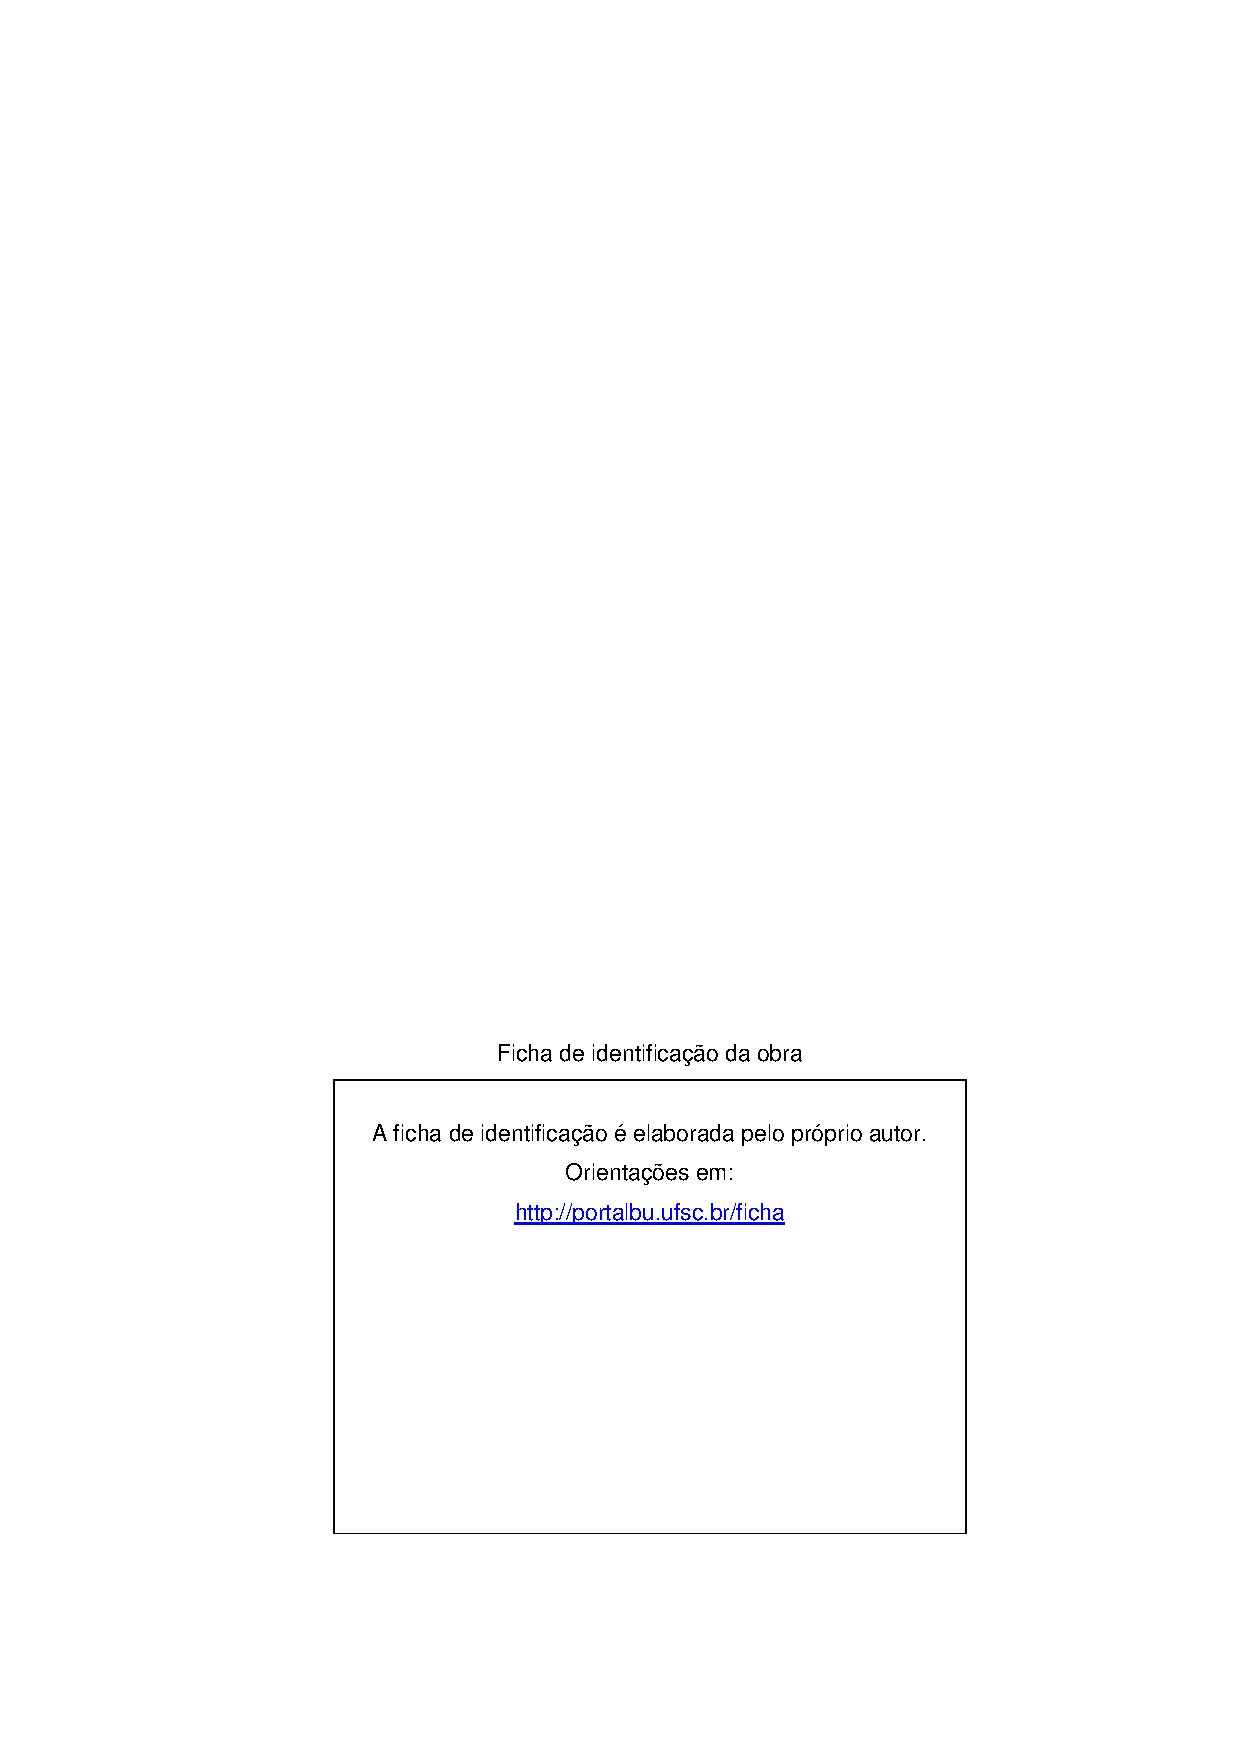
\includepdf{pictures/Ficha_Catalografica.pdf}
    \ifforcedinclude\else\cleardoublepage\fi
\fi


% Inserir errata

% Inserir folha de aprovação. Isto é um exemplo de Folha de aprovação, elemento obrigatório da
% NBR 14724/2011 (seção 4.2.1.3). Você pode utilizar este modelo até a aprovação do trabalho.
% Após isso, substitua todo o conteúdo deste arquivo por uma imagem da página assinada pela
% banca com o comando abaixo:
\ifforcedinclude\else\cleardoublepage\fi


\addtotextpreliminarycontent{\lang{Approval Sheet}{Folha de Aprovação}}

\begin{folhadeaprovacao}

    \begin{center}
        {\imprimirautor}

        \begin{center}
            \ABNTEXchapterfont\bfseries\MakeUppercase{\imprimirtitulo}\ifnotempty{\imprimirsubtitulo}{: \imprimirsubtitulo}
        \end{center}

        \begin{minipage}{\textwidth}
            \lang
            {
                This \imprimirtipotrabalho~was considered appropriate to get the \imprimirformacao,
                \ifnotempty{\imprimirarea}{in the area of \imprimirarea,}
                and it was approved by the \imprimirprograma~of \imprimircentro~of \imprimirinstituicao.
            }
            {
                Este(a) \imprimirtipotrabalho~foi julgado adequado(a) para obtenção do Título de \imprimirformacao,
                \ifnotempty{\imprimirarea}{na área de concentração de \imprimirarea,}
                e foi aprovado em sua forma final pelo \imprimirprograma~
                do \imprimircentro~da \imprimirinstituicao.
            }
         \end{minipage}%
    \end{center}

    \begin{center}
        \imprimirlocal, \imprimirdata.
    \end{center}

    \assinatura{%
        \textbf{\imprimircoordenador} \\
        \imprimircoordenadorRotulo~\lang{of}{do} \imprimirprograma
    }

    % \newpage
    \begin{flushleft}
        \textbf{\lang{Examination Board}{Banca Examinadora}:}
    \end{flushleft}

    \assinatura{%
        \textbf{\imprimirorientador} \\ \imprimirorientadorRotulo\\
        \imprimirinstituicao~--~\imprimirinstituicaosigla
    }

    \ifnotempty{\imprimircoorientador}{%
        \assinatura{%
            \textbf{\imprimircoorientador} \\ \imprimircoorientadorRotulo \\
            \imprimirinstituicao~--~\imprimirinstituicaosigla
        }
    }

    \assinatura{%
        \textbf{Antonio Felipe Da Cunha De Aquino, \lang{PhD.}{Dr.}} \\
        Universidade Federal de Santa Catarina -- UFSC
    }

    \assinatura{%
        \textbf{Heitor José Tessaro, \lang{Ms.}{Me.}} \\
        Universidade Federal de Santa Catarina -- UFSC
    }

\end{folhadeaprovacao}


% \includepdf{pictures/folhadeaprovacao_final.pdf}


% Dedicatória
\ifforcedinclude\else\cleardoublepage\fi
\ifforcedinclude\else

\addtotextpreliminarycontent{\lang{Dedicatory}{Dedicatória}}

\begin{dedicatoria}

    \vspace*{\fill}
    \centering
    \noindent
    \textit{\lang
    {
        This work is dedicated to adult children who, \\
        When small, dreamed of becoming scientists.
    }
    {
        Este trabalho é dedicado às crianças adultas que,\\
        quando pequenas, sonharam em se tornar cientistas.
    }}
    \vspace*{\fill}

\end{dedicatoria}


\fi

% Agradecimentos
\ifforcedinclude\else\cleardoublepage\fi


\addtotextpreliminarycontent{\lang{Acknowledgement}{Agradecimentos}}

\begin{agradecimentos}

\lang
{
    Greetings.
}
{
Os principais agradecimentos deste trabalho são direcionados aos meus pais, Luiz e Rosinete, e minha irmã, Laiana, por nunca terem me deixado desistir dos meus sonhos. Agradecimentos especiais ao orientador Miguel Moreto, pelo incentivo e direcionamento excepcionais, e aos colegas e amigos da Reason, em especial a Elias Bencz e Hector De La Hoz pelas valiosas conversas técnicas e filosóficas. Por fim, agradecimentos a todos os amigos que vida me trouxe e que fez questão de manter: foram os sorrisos que vocês trouxeram que permitiram a execução deste trabalho.
}

\end{agradecimentos}


%Mesmo padrão da seção primária, porém sem indicativo numérico. Assim como: Dedicatória, Resumo, Abstract, Sumário, Listas, Referências, Apêndices e Anexos.
%
%
%Corpo do texto, fonte 10,5, justificado, recuo especial da primeira linha de 1 cm, espaçamento simples.
%


% Epígrafe
\ifforcedinclude\else\cleardoublepage\fi


\addtotextpreliminarycontent{\lang{Epigraph}{Epigrafe}}

\begin{epigrafe}

\vspace*{\fill}\lang
{
    \begin{flushright}
        \textit{``Learn from yesterday, live for today, hope for tomorrow. The important thing is not to stop questioning.''} \\ Albert Einstein
    \end{flushright}
    \begin{flushright}
        \textit{``The true sign of intelligence is not knowledge but imagination.''} \\  Albert Einstein
    \end{flushright}
    \begin{flushright}
        \textit{``Peace cannot be kept by force; it can only be achieved by understanding.''} \\ Albert Einstein
    \end{flushright}
    \begin{flushright}
        \textit{``Whoever is careless with the truth in small matters cannot be trusted with important matters.''} \\ Albert Einstein
    \end{flushright}
    \begin{flushright}
        \textit{``Extraordinary claims require extraordinary evidence''} \\ Carl Sagan
    \end{flushright}
    \begin{flushright}
        \textit{``Catholic, which I was until I reached the age of reason.''} \\ George Carlin
    \end{flushright}
    \begin{flushright}
        \textit{``We made too many wrong mistakes.''} \\ Yogi Berra
    \end{flushright}
}
{
    \begin{flushright}
        \textit{``I have not failed. I've just found 10,000 ways that won't work.''} \\ Thomas Alva Edison
    \end{flushright}
}

\end{epigrafe}





% Ajusta o espaçamento dos parágrafos do resumo
\setlength{\absparsep}{18pt}

% RESUMOS
\ifforcedinclude\else\cleardoublepage\fi


\newcommand{\imprimirbrazilabstract}{%
    \cleardoublepage\phantomsection
    \addtotextpreliminarycontent{Resumo em Português}
    \begin{otherlanguage*}{brazil}
    \begin{resumo}[Resumo]

        Segundo a \textcite[3.1-3.2]{NBR6028:2003}, o resumo deve ressaltar o
        objetivo, o método, os resultados e as conclusões do documento. A ordem e a extensão
        destes itens dependem do tipo de resumo (informativo ou indicativo) e do
        tratamento que cada item recebe no documento original. O resumo deve ser
        precedido da referência do documento, com exceção do resumo inserido no
        próprio documento. (\ldots) As palavras-chave devem figurar logo abaixo do
        resumo, antecedidas da expressão Palavras-chave:, separadas entre si por
        ponto e finalizadas também por ponto.

        Além disso, na UFSC o texto do resumo deve ser digitado, em um único bloco, sem espaço de parágrafo. O resumo deve
        ser significativo, composto de uma sequência de frases concisas, afirmativas e não de uma
        enumeração de tópicos. Não deve conter citações. Deve usar o verbo na voz passiva. Abaixo do
        resumo, deve-se informar as palavras-chave (palavras ou expressões significativas retiradas do
        texto) ou, termos retirados de thesaurus da área. \englishword{\showfont}

        \imprimirpalavraschave{Palavras-chaves}{\begin{inparaitem}[]\palavraschaveportugues\end{inparaitem}}

    \end{resumo}
    \end{otherlanguage*}
}


\newcommand{\imprimirenglishabstract}{%
    % https://tex.stackexchange.com/questions/20987/changing-babel-package-inside-a-single-chapter
    % https://tex.stackexchange.com/questions/36526/multiple-language-document-babel-selectlanguage-vs-begin-endotherlanguage
    \cleardoublepage\phantomsection
    \addtotextpreliminarycontent{English's Abstract}
    \begin{otherlanguage*}{english}
    \begin{resumo}[Abstract]

        This is the English abstract.

        \imprimirpalavraschave{Keywords}{\begin{inparaitem}[]\palavraschaveingles\end{inparaitem}}

    \end{resumo}
    \end{otherlanguage*}
}


% \newcommand{\imprimirfrenchabstract}{%
%     \addtotextpreliminarycontent{Français Résumé}
%     \begin{resumo}[Résumé]
%       \begin{otherlanguage*}{french}
%           Il s'agit d'un résumé en français.

%           \imprimirpalavraschave{Mots-clés}{latex. abntex. publication de textes.}
%       \end{otherlanguage*}
%     \end{resumo}
% }


% \newcommand{\imprimirspanishabstract}{%
%     \addtotextpreliminarycontent{Español Resumen}
%     \begin{resumo}[Resumen]
%       \begin{otherlanguage*}{spanish}
%           Este es el resumen en español.

%           \imprimirpalavraschave{Palabras clave}{latex. abntex. publicación de textos.}
%       \end{otherlanguage*}
%     \end{resumo}
% }


\makeatletter
\ifenglish
    \@ifundefined{imprimirbrazilabstract}{}{\imprimirbrazilabstract}

    % https://tex.stackexchange.com/questions/331108/times-new-roman-in-latex-just-some-text
    % https://tex.stackexchange.com/questions/11707/how-to-force-output-to-a-left-or-right-page
    % https://tex.stackexchange.com/questions/132966/do-not-display-chapter-title-in-memoir-class
    \cleardoublepage\phantomsection
    \pretextualchapter{Resumo Expandido}
    \addtotextpreliminarycontent{Resumo Expandido}

    \begin{otherlanguage*}{brazil}
        \setlength{\parskip}{0.2cm}
        \setlength{\parindent}{0.0cm}
        \fontfamily{ptm}\selectfont

        \section*{Introdução}
        O resumo expandido é previsto na Resolução Normativa nº 95/CUn/2017, Art. 55, § 2, de 4 de
        abril de 2017, e exigido para teses e dissertações escritas em idiomas estrangeiros (com
        exceção dos cursos pertinentes ao estudo de idiomas estrangeiros – Programa de Pós-Graduação
        em Estudos da Tradução e Programa de Pós-Graduação em Inglês: Estudos Linguísticos e
        Literários).

        O resumo expandido é considerado um elemento pré-textual e deverá ser incluído no trabalho
        após o resumo e antes do abstract. Deverá iniciar em página impar (no anverso de uma folha)
        continuando no verso da folha. O texto deverá seguir o formato A5, com margens espelhadas:
        superior 2,0 cm, inferior 1,5 cm, interna 2,5 cm e externa 1,5. Deve ser empregada a fonte
        Time New Roman.  Todo o texto deve ser digitado em tamanho 10,5. O espaçamento entre as
        linhas deverá ser simples. A expressão “resumo expandido” deve seguir a mesma tipografia das
        demais sessões primárias do trabalho.

        O texto do resumo expandido deve ser redigido em português e conter as seguintes seções (ver
        modelo): Introdução, Objetivos, Metodologia, Resultados e Discussão e Considerações Finais.
        Deve apresentar no mínimo duas (02) e, no máximo, cinco (05) páginas contendo a mesma
        formatação em A5 do resumo e do abstract, bem como palavras-chave. \englishword{\showfont}

        \section*{Objetivos}
        Lorem ipsum dolor sit amet, consectetur adipiscing elit. Phasellus vitae dolor lacus. Ut
        accumsan vitae felis nec porttitor. Integer interdum fringilla feugiat. Nullam pulvinar sit
        amet tellus eget maximus. Donec sit amet magna eget justo semper fermentum vel eget velit.
        In iaculis imperdiet mauris, ac ornare libero placerat non. Nulla libero lectus, ullamcorper
        ac ornare eget, pulvinar ac nulla. Curabitur vestibulum non nisl eget sagittis. Proin
        gravida lacus id eros bibendum interdum. Mauris ullamcorper elementum tortor sed consequat.
        Integer tempus, est a lobortis vehicula, nisi mi fringilla augue, non semper leo metus in
        quam. Etiam in leo maximus, pulvinar mi eget, vehicula risus. Donec sed dui semper, dictum
        eros at, suscipit felis.

        Nam sagittis vel orci at tempus. Nulla non pellentesque eros.
        Quisque cursus leo massa, eu ultricies nisl lacinia a. Nulla sit amet elementum ligula.
        Proin sodales venenatis dictum. Ut et est cursus, vulputate velit et, viverra odio. Interdum
        et malesuada fames ac ante ipsum primis in faucibus. Maecenas purus diam, tempor a semper
        et, finibus a ex. Cras sagittis felis urna, et consequat arcu lacinia ut. Praesent blandit
        venenatis ante nec porta. Duis rutrum, tellus vitae ullamcorper auctor, lectus ex laoreet
        est, ac tristique ipsum arcu vitae nibh. Nam efficitur felis ut mi consectetur, nec auctor
        odio ornare. In tempor vulputate urna, vitae cursus enim egestas eu. Proin diam augue,
        dignissim vitae ligula eget, lobortis ornare odio. Duis quis elit augue. Fusce quis rhoncus
        tortor. Donec hendrerit at massa a mattis. Sed ipsum neque, aliquam ut sem sed, ultrices
        varius ligula. Suspendisse blandit, dolor ac rhoncus lacinia, dolor purus cursus purus, et
        accumsan orci neque a leo.

        \section*{Metodologia}
        Quisque efficitur dolor in lectus dapibus elementum. Nam ultrices blandit consectetur.
        Nullam ultricies sit amet odio quis placerat. Aenean eget est elit. Maecenas et nulla dolor.
        Orci varius natoque penatibus et magnis dis parturient montes, nascetur ridiculus mus. In
        pulvinar velit sed mi sagittis ornare. Aenean rutrum suscipit egestas. Phasellus pharetra
        eget ex in volutpat. Quisque eu arcu nunc. Vivamus arcu ligula, pharetra at rhoncus sit
        amet, pulvinar sed eros. Sed porta ipsum ipsum, et fermentum magna volutpat sed. Vivamus
        pharetra facilisis orci, sit amet luctus nisl pretium id. Sed consequat, arcu et congue
        pulvinar, risus enim aliquet purus, eget venenatis libero leo sit amet metus. Maecenas vitae
        elit sapien. Fusce mollis libero et gravida placerat. Proin ut quam quis justo aliquam
        dictum. Donec volutpat convallis suscipit. Vivamus metus nisl, placerat ac enim vitae,
        tempus ultricies odio.

        Aliquam ac vehicula arcu, non bibendum nulla. Morbi libero sem,
        imperdiet vel quam et, posuere tempus nunc. Maecenas dictum magna sit amet ligula facilisis
        commodo. Aliquam tellus diam, ornare vel elementum in, dignissim id purus. Ut at tortor non
        sem molestie euismod non at turpis. Phasellus vitae bibendum tellus. Suspendisse odio enim,
        faucibus eget congue quis, semper sit amet tortor. Sed ac lectus est. Pellentesque nec
        mattis mi, et varius dolor. Aliquam quis massa ac tellus malesuada sollicitudin. Maecenas
        ultrices risus massa, nec auctor risus sagittis id. Praesent a sapien nulla. Donec
        tincidunt, metus quis hendrerit facilisis, enim augue convallis elit, sed consequat lacus
        odio vitae magna.

        \section*{Resultados e Discussão}
        Nullam sed cursus leo. Donec commodo volutpat hendrerit. Fusce et tempus lectus, feugiat
        consequat est. Class aptent taciti sociosqu ad litora torquent per conubia nostra, per
        inceptos himenaeos. Nam quis cursus mauris, non tempus orci. Phasellus lobortis et mauris at
        vulputate. Sed nec nisl elementum lorem commodo gravida non a enim. Phasellus neque erat,
        aliquet ac ligula ac, maximus vestibulum sem. Vestibulum vel tincidunt turpis. Donec lacinia
        rutrum dolor dapibus bibendum. Mauris pharetra nibh nec tincidunt iaculis. Vivamus pharetra
        bibendum nisl eget blandit. In lobortis diam non justo eleifend, id lobortis ante fringilla.
        Donec libero tortor, suscipit vestibulum vestibulum id, rutrum accumsan turpis. Phasellus
        sollicitudin luctus tincidunt. Suspendisse potenti. Nam semper metus et mi pharetra, in
        pretium ligula fermentum. Integer consectetur, orci non placerat feugiat, dui ex gravida
        augue, vel placerat ligula augue vel velit. Aliquam sollicitudin pellentesque congue. Donec
        vitae turpis in ante posuere posuere. Pellentesque eu justo leo. Donec quis elit vitae leo
        varius luctus quis eget justo.

        Vestibulum elementum ex neque, quis commodo tortor porttitor
        mattis. Mauris vel sagittis turpis. Aenean ligula turpis, eleifend at felis sed, cursus
        condimentum orci. Fusce accumsan est odio, eu venenatis massa sodales in. Curabitur a tempor
        nisl. Quisque consequat sed arcu a congue. In viverra, ex ut hendrerit condimentum, urna sem
        euismod eros, nec suscipit turpis dolor eget augue. Aenean posuere tellus et consectetur
        condimentum. Mauris et massa et nulla fringilla interdum. Duis quis posuere elit. Donec at
        ex non arcu faucibus rutrum et vel lectus. Vivamus pellentesque vestibulum rutrum. Sed
        pretium, purus sed efficitur feugiat, nisi justo eleifend nibh, id suscipit nunc massa nec
        lectus. In euismod enim eu sapien dictum sodales. Fusce sit amet vulputate orci. Nulla
        rutrum mauris at purus aliquet, ac sollicitudin leo laoreet. Etiam elementum posuere
        feugiat. Maecenas sed libero non augue fermentum ultricies eget at mi. Aenean auctor
        bibendum lacus, dignissim aliquet est tempus eget. Maecenas tempus, nulla id rhoncus
        suscipit, augue leo auctor mi, eget tincidunt magna mi quis dui. Maecenas ut elit in turpis
        tincidunt ultrices. Nulla id nulla aliquet, porttitor eros quis, egestas justo. Nunc nisi
        quam, egestas a accumsan fermentum, ultricies ac elit.

        Nulla porta auctor vestibulum. Sed
        consectetur lacus molestie iaculis ullamcorper. Proin porta posuere massa a lacinia. Nunc a
        lacinia orci, non vehicula ante. Vestibulum ipsum velit, congue et neque aliquam, imperdiet
        ornare augue. Donec et congue sapien. Pellentesque consequat consectetur neque ut varius. In
        aliquam ex quis ante venenatis dapibus. Vivamus et imperdiet urna. Vestibulum quis nibh
        magna. In a congue lectus, eu sodales nunc. Suspendisse id.

        \section*{Considerações Finais}
        Lorem ipsum dolor sit amet, consectetur adipiscing elit. Phasellus vitae dolor lacus. Ut
        accumsan vitae felis nec porttitor. Integer interdum fringilla feugiat. Nullam pulvinar sit
        amet tellus eget maximus. Donec sit amet magna eget justo semper fermentum vel eget velit.
        In iaculis imperdiet mauris, ac ornare libero placerat non. Nulla libero lectus, ullamcorper
        ac ornare eget, pulvinar ac nulla. Curabitur vestibulum non nisl eget sagittis. Proin
        gravida lacus id eros bibendum interdum. Mauris ullamcorper elementum tortor sed consequat.
        Integer tempus, est a lobortis vehicula, nisi mi fringilla augue, non semper leo metus in
        quam. Etiam in leo maximus, pulvinar mi eget, vehicula risus. Donec sed dui semper, dictum
        eros at, suscipit felis.

        Nam sagittis vel orci at tempus. Nulla non pellentesque eros.
        Quisque cursus leo massa, eu ultricies nisl lacinia a. Nulla sit amet elementum ligula.
        Proin sodales venenatis dictum. Ut et est cursus, vulputate velit et, viverra odio. Interdum
        et malesuada fames ac ante ipsum primis in faucibus. Maecenas purus diam, tempor a semper
        et, finibus a ex. Cras sagittis felis urna, et consequat arcu lacinia ut. Praesent blandit
        venenatis ante nec porta. Duis rutrum, tellus vitae ullamcorper auctor, lectus ex laoreet
        est, ac tristique ipsum arcu vitae nibh. Nam efficitur felis ut mi consectetur, nec auctor
        odio ornare. In tempor vulputate urna, vitae cursus enim egestas eu. Proin diam augue,
        dignissim vitae ligula eget, lobortis ornare odio. Duis quis elit augue. Fusce quis rhoncus
        tortor. Donec hendrerit at massa a mattis. Sed ipsum neque, aliquam ut sem sed, ultrices
        varius ligula. Suspendisse blandit, dolor ac rhoncus lacinia, dolor purus cursus purus, et
        accumsan orci neque a leo.


        \imprimirpalavraschave{Palavras-chaves}{\begin{inparaitem}[]\palavraschaveportugues\end{inparaitem}}

    \end{otherlanguage*}

    \@ifundefined{imprimirenglishabstract}{}{\imprimirenglishabstract}

\else
    \@ifundefined{imprimirbrazilabstract}{}{\imprimirbrazilabstract}
    \@ifundefined{imprimirenglishabstract}{}{\imprimirenglishabstract}
\fi

\@ifundefined{imprimirfrenchabstract}{}{\imprimirfrenchabstract}
\@ifundefined{imprimirspanishabstract}{}{\imprimirspanishabstract}
\makeatother



% Some tables of contents
\ifforcedinclude\else
{
    % https://tex.stackexchange.com/questions/179506/disable-colorlinks-locally-or-just-for-the-toc
    \hypersetup{hidelinks}

    % inserir lista de figuras
    \ifforcedinclude\else\cleardoublepage\fi
    % https://tex.stackexchange.com/questions/234398/list-of-figures-and-tables-when-there-are-no-figures-or-tables
    \whenlistisnotempty{\listfigurename}{%
        \addtotextpreliminarycontent{\listfigurename}
        % https://tex.stackexchange.com/questions/121879/remove-spacing-between-per-chapter-figures-in-lof
        {\renewcommand{\addvspace}[1]{}
        \listoffigures*}
    }{\pdfbookmark[0]{\listfigurename}{lof}}

    % inserir lista de quadros
    \ifforcedinclude\else\cleardoublepage\fi
    % https://tex.stackexchange.com/questions/234398/list-of-figures-and-tables-when-there-are-no-figures-or-tables
    \whenlistisnotempty{\listofquadrosname}{%
        \addtotextpreliminarycontent{\listofquadrosname}
        % https://tex.stackexchange.com/questions/121879/remove-spacing-between-per-chapter-figures-in-lof
        {\renewcommand{\addvspace}[1]{}
        \listofquadros*}
    }{\pdfbookmark[0]{\listofquadrosname}{loq}}

    % inserir lista de tabelas
    \ifforcedinclude\else\cleardoublepage\fi
    % https://tex.stackexchange.com/questions/234398/list-of-figures-and-tables-when-there-are-no-figures-or-tables
    \whenlistisnotempty{\listtablename}{%
        \addtotextpreliminarycontent{\listtablename}
        % https://tex.stackexchange.com/questions/121879/remove-spacing-between-per-chapter-figures-in-lof
        {\renewcommand{\addvspace}[1]{}
        \listoftables*}
    }{\pdfbookmark[0]{\listtablename}{lot}}

    % inserir códigos fonte (List of Listings `lol`)
    % https://tex.stackexchange.com/questions/511519/latex-keeps-showing-minted-environment-as-figures-instead-of-listening/511579#511579
    \ifforcedinclude\else\cleardoublepage\fi
    % https://tex.stackexchange.com/questions/234398/list-of-figures-and-tables-when-there-are-no-figures-or-tables
    \whenlistisnotempty{\lstlistlistingname}{%
        \addtotextpreliminarycontent{\lstlistlistingname}
        % https://tex.stackexchange.com/questions/121879/remove-spacing-between-per-chapter-figures-in-lof
        {\renewcommand{\addvspace}[1]{}
        \lstlistoflistings*}
    }{\pdfbookmark[0]{\lstlistlistingname}{lol}}
}
\fi


% inserir lista de abreviaturas e siglas
\ifforcedinclude\else\cleardoublepage\fi


\addtotextpreliminarycontent{\lang{List of Acronyms}{Lista de Siglas}}

\begin{siglas}
    \item[ABNT] \lang{Brazilian Association of Technical Standards}{Associação Brasileira de Normas Técnicas}
    \item[abnTeX] \lang{Absurd Standards for TeX}{ABsurdas Normas para TeX}
\end{siglas}



% Inserir lista de símbolos
\ifforcedinclude\else\cleardoublepage\fi


\addtotextpreliminarycontent{\lang{List of Symbols}{Lista de Símbolos}}

% Devam aparecer na mesma ordem de ocorrência no texto.
\begin{simbolos}
    \item[$ \Gamma $] \lang{Greek letter Gama}{Letra grega Gama}
    \item[$ \Lambda $] \lang{Lambda}{Lambda}
    \item[$ \zeta $] \lang{Minimal Greek letter zeta}{Letra grega minúscula zeta}
    \item[$ \in $] \lang{Belongs}{Pertence}
\end{simbolos}


% How to remove the self-reference of the ToC from the ToC?
% https://tex.stackexchange.com/questions/10943/how-to-remove-the-self-reference-of-the-toc-from-the-toc
\ifforcedinclude\else\cleardoublepage\fi

\begin{KeepFromToc}
    % https://tex.stackexchange.com/questions/35/what-does-overfull-hbox-mean
    % https://tex.stackexchange.com/questions/59122/how-to-avoid-using-sloppy-document-wide-to-fix-overfull-hbox-problems
    % https://tex.stackexchange.com/questions/257007/adding-color-to-table-of-contents-and-section-headings
    {
        % https://tex.stackexchange.com/questions/179506/disable-colorlinks-locally-or-just-for-the-toc
        \hypersetup{hidelinks}

        % https://tex.stackexchange.com/questions/65711/underfull-vbox-badness-10000-with-memoir
        \raggedbottom

        % https://tex.stackexchange.com/questions/49887/overfull-hbox-warning-for-toc-entries-when-using-memoir-documentclass
        % \makeatletter
            % \renewcommand{\@pnumwidth}{2em}
            % \renewcommand{\@tocrmarg}{3em}
        % \makeatother

        % https://tex.stackexchange.com/questions/57544/memoir-mysterious-overfull-hbox-in-toc-when-mathptmx-is-used
        % \setlength{\cftchapternumwidth}{2.25em}

        % Add the table of contents to the brief table of contents
        % https://tex.stackexchange.com/questions/234398/list-of-figures-and-tables-when-there-are-no-figures-or-tables
        \whenlistisnotempty{\contentsname}{%
            \addtotextpreliminarycontent{\contentsname}
            \tableofcontents
        }{\pdfbookmark[0]{\contentsname}{toc}}
    }

\end{KeepFromToc}



    % ELEMENTOS TEXTUAIS
    \textual
    \setlength\beforechapskip{50pt}
    \setlength\midchapskip{20pt}
    \setlength\afterchapskip{20pt}

    % PARTE
 %   \ifforcedinclude\else\part{\lang{Research}{Pesquisa}}\fi
  %  \label{primeira_parte}

    % Introdução (exemplo de capítulo sem numeração, mas presente no Sumário)
    %% intro.tex
%%
%% Copyright 2017 Evandro Coan
%% Copyright 2012-2016 by abnTeX2 group at http://www.abntex.net.br/
%%
%% This work may be distributed and/or modified under the
%% conditions of the LaTeX Project Public License, either version 1.3
%% of this license or (at your option) any later version.
%% The latest version of this license is in
%%   http://www.latex-project.org/lppl.txt
%% and version 1.3 or later is part of all distributions of LaTeX
%% version 2005/12/01 or later.
%%
%% This work has the LPPL maintenance status `maintained'.
%% The Current Maintainer of this work is the Evandro Coan.
%%
%% The last Maintainer of this work was the abnTeX2 team, led
%% by Lauro César Araujo. Further information are available on
%% https://www.abntex.net.br/
%%
%% This work consists of a bunch of files. But originally there ware 3 files
%% which are renamed as follows:
%% Renamed the `abntex2-modelo-include-comandos` to `chapters/chapter_1.tex`
%% Renamed the `abntex2-modelo-trabalho-academico.tex` to `chapters/intro.tex`
%% Renamed the `abntex2-modelo-references.bib` to `aftertext/modelo-ufsc-references.bib`
%%
%% This file was originally the main template file, however this main file was
%% split into several new files, which are respectively drastically changed,
%% except this files which contains most of the main documentation message.
%%

% ------------------------------------------------------------------------
% ------------------------------------------------------------------------
% abnTeX2: Modelo de Trabalho Academico (tese de doutorado, dissertacao de
% mestrado e trabalhos monograficos em geral) em conformidade com
% ABNT NBR 14724:2011: Informacao e documentacao - Trabalhos academicos -
% Apresentacao
% ------------------------------------------------------------------------
% ------------------------------------------------------------------------

% The \phantomsection command is needed to create a link to a place in the document that is not a
% figure, equation, table, section, subsection, chapter, etc.
% https://tex.stackexchange.com/questions/44088/when-do-i-need-to-invoke-phantomsection
\phantomsection

% https://tex.stackexchange.com/questions/5076/is-it-possible-to-keep-my-translation-together-with-original-text
\chapter{\lang{Introduction}{Introdução}}
\phantomsection

Um dos marcos mais importantes na linha evolutiva das subestações elétricas foi a digitalização dos dados de medição e proteção oriundos dos transformadores de instrumentação, bem como a própria digitalização de todas as redes de controle e monitoração. A partir deste momento, as redes de comunicação entre os equipamentos da subestação deixaram de ser totalmente analógicas e foram substituídas gradativamente por protocolos digitais que trazem maior robustez, confiabilidade e segurança. Da mesma forma, os sinais de corrente e tensão vindos dos transformadores de instrumentação também passaram a ser discretizados e amostrados em pacotes, seguindo normas internacionais de estrutura, precisão e organização. As subestações que possuem esta características implementadas são chamadas de Subestações Elétricas Digitais.

Neste contexto, as \textit{Merging Units} são equipamentos essenciais para a interface entre os transformadores de instrumentação e os IEDs (\textit{Intelligent Electronic Devices}), como relés de proteção, gravadores digitais (\textit{Digital Recorders}) e localizadores de falhas (\textit{Fault Locators}). Estes equipamentos são responsáveis pela ``ponte'' entre a parte analógica e a parte digital de uma subestação elétrica. Na captura dos sinais de tensão e corrente advindos dos transformadores, os erros máximos de magnitude expostos na documentação do fabricante devem ser respeitados ao longo de toda a faixa de aquisição do equipamento.

%adicionar mais informações sobre merging units // tendência da digitalização das subestações // de onde vai e pra onde vem

Uma vez que estes erros máximos não são garantidos apenas pelo projeto de \textit{hardware} do equipamento, a motivação deste trabalho surge da necessidade de calibração das placas de aquisição analógica de corrente e tensão das \textit{Merging Units}. Nesta esfera, a norma IEC 61850-7-2 \cite{IEC61850_7-2} traz os \textit{Sampled Values} como formato padrão para sinais elétricos e é através destes que este trabalho pretende calcular os ganhos e \textit{offsets} necessários para manter os canais de aquisição de tensão e corrente dentro das especificações propostas pelo fabricante, também em consonância com o que é proposto pela norma IEC 61869-13 \cite{IEC61869-13}. 

\section{Objetivos}

Com este plano de fundo, este trabalho tem como objetivo geral propor uma metodologia de calibração para as placas de aquisição analógica de \textit{Merging Units}, de forma a reduzir os erros de magnitude das leituras e adequar os canais aos padrões pré-estabelecidos.

Para atender ao objetivo geral, podem ser elencados os seguintes objetivos específicos:

\begin{itemize}
    \item Captura e processamento dos pacotes de \textit{Sampled Values} \cite{IEC61850-9-2} gerados pela \textit{Merging Unit} a partir de sinais de corrente e tensão aplicados nos seus canais de aquisição analógica;
    \item Conversão dos pacotes \textit{Sampled Values} em arquivos \textit{COMTRADE} \cite{comtrade1992} e avaliação dos seus erros em relação ao sinal aplicado antes das calibrações;
    \textit Implementação dos métodos de calibração;
    \item Utilização dos \textit{COMTRADEs} gerados como entrada para os métodos de calibração, de forma a obter como saída os coeficientes de linearização;
    \item Aplicação dos coeficientes nos \textit{COMTRADEs}, a fim de avaliar os resultados de cada um dos métodos.
\end{itemize}


\section{Estrutura do Trabalho}

Este trabalho é dividido em três capítulos: o primeiro introduz cada um dos métodos utilizados para a calibração dos canais de aquisição analógica da \textit{Merging Unit}, mostrando seus equacionamentos, vantagens e desvantagens. O segundo capítulo mostra como a metodologia proposta neste trabalho, utilizando os métodos do primeiro capítulo, é utilizada para obter os coeficientes de calibração para os canais de corrente e de tensão. Por sua vez, o terceiro capítulo mostra os resultados da aplicação da metodologia de calibração proposta em uma \textit{Merging Unit} real, utilizando sinais em 50 Hz e 60 Hz.











    % Capitulo com exemplos de comandos inseridos de arquivo externo
    %% chapters/chapter_1.tex
%%
%% Copyright 2017 Evandro Coan
%% Copyright 2012-2014 by abnTeX2 group at http://abntex2.googlecode.com/
%%
%% This work may be distributed and/or modified under the
%% conditions of the LaTeX Project Public License, either version 1.3
%% of this license or (at your option) any later version.
%% The latest version of this license is in
%%   http://www.latex-project.org/lppl.txt
%% and version 1.3 or later is part of all distributions of LaTeX
%% version 2005/12/01 or later.
%%
%% This work has the LPPL maintenance status `maintained'.
%%
%% The Current Maintainer of this work is the Evandro Coan.
%%
%% The last Maintainer of this work was the abnTeX2 team, led
%% by Lauro César Araujo. Further information are available on
%% https://www.abntex.net.br/
%%
%% This work consists of a bunch of files. But originally there were 2 files
%% which are renamed as follows:
%% Deleted the `abntex2-modelo-img-marca.pdf`
%% Renamed the `abntex2-modelo-include-comandos.tex, v-1.9.2 laurocesar` to `chapters/chapter_1.tex`
%%
% ---
% Este capítulo, utilizado por diferentes exemplos do abnTeX2, ilustra o uso de
% comandos do abnTeX2 e de LaTeX.
% ---

% The \phantomsection command is needed to create a link to a place in the document that is not a
% figure, equation, table, section, subsection, chapter, etc.
% https://tex.stackexchange.com/questions/44088/when-do-i-need-to-invoke-phantomsection
\phantomsection

% https://tex.stackexchange.com/questions/5076/is-it-possible-to-keep-my-translation-together-with-original-text
\chapter[\lang{Algorithms Presentation}{Algoritmos de calibração utilizados}]
{
    \lang
    {Calibration Algorithms used}
    {Algoritmos de calibração utilizados}
}

\label{cap_algoritmos}


%\begin{flushright}
%    \englishword{\showfont}
%\end{flushright}

% Why latex is letting my text goes out of the screen?
% https://tex.stackexchange.com/questions/386762/why-latex-is-letting-my-text-goes-out-of-the-screen
%\sloppy
%\textbf{textbf: \englishword{\showfont}}
%\fussy


\section{Linearização por mínimos quadrados ordinários - \textit{Ordinary Least Squares}}

Este primeiro método baseia-se no princípio dos mínimos quadrados para obtenção dos parâmetros desconhecidos (ou coeficientes) de um modelo de regressão linear: minimizar a soma dos quadrados das diferenças entre os valores observados em determinado conjunto de dados e os valores preditos pela função linear da variável independente.

De forma geométrica, este método pode ser visto como a soma das distâncias ao quadrado entre cada ponto no grupo de dados adquiridos e o seu ponto correspondente na função de regressão. Quanto menor essa distância, melhor o modelo se ajusta aos dados.

Para compreender o método matematicamente, partimos da definição de regressão linear, pois este conceito é importante não apenas para o método de Mínimos quadrados ordinários, mas para a compreensão de todos os outros métodos citados neste trabalho: regressão linear é um modelo estatístico utilizado para estimar o valor esperado de uma variável \textit{y}, dados os valores de outras variáveis \textit{x}, através da seguinte fórmula \cite{ols_intro_econometrics}:

\begin{equation}\label{eq:1}
y_i = \alpha + \beta x_i + \epsilon_i
\end{equation}

Onde \textit{y} é a variável a ser estimada, \textit{x} é a variável que deverá ser capaz de estimar \textit{y}, $\alpha$ é o parâmetro independente de \textit{x} e  $\beta$ é o coeficiente da variável \textit{x}. No caso em estudo, onde existem \textit{n} amostras a serem utilizadas nessa linearização, \textit{x} e \textit{y} serão vetores de tamanho \textit{n}.

Graficamente, essa linearização pode ser exemplificada pela figura \ref{fig:ols_1}, que ilustra cada um dos termos da equação, bem como a própria linha regressora:

\begin{figure}[htp]
    \centering
    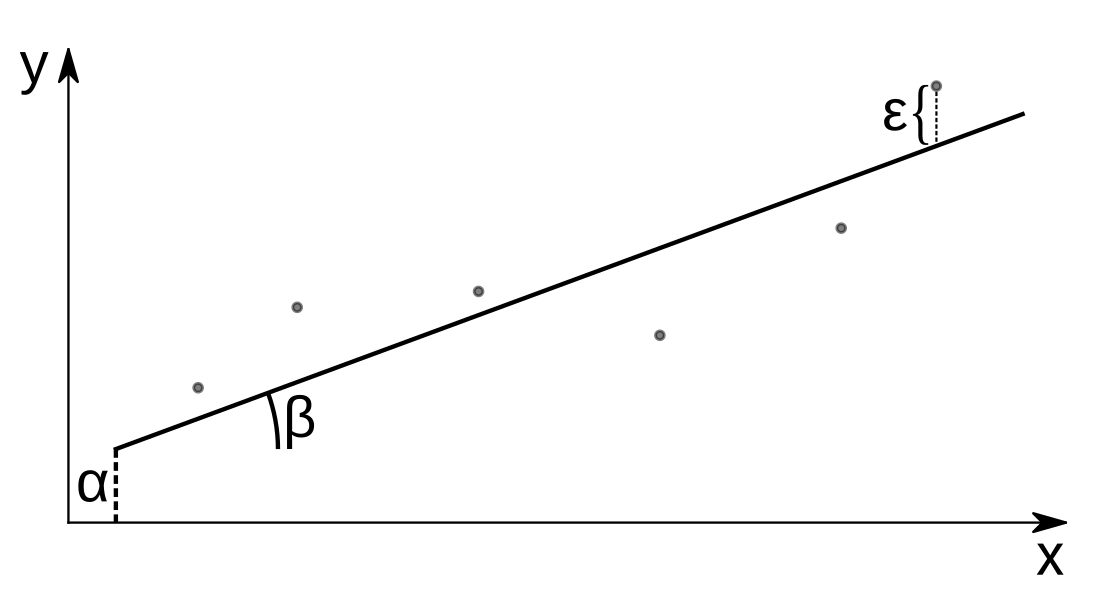
\includegraphics[width=12cm]{lsq.png}
    \caption{Representação gráfica da linearização por mínimos quadrados ordinários}
    \label{fig:ols_1}
\end{figure}

Matricialmente, a equação \ref{eq:1} pode ser exposta da forma:

\begin{equation*} \textbf{Y}= \alpha + \textbf{X}\beta+\epsilon, \end{equation*}

Onde \textbf{Y} representa o vetor de valores a serem estimados, \textbf{X} representa o vetor de dados observados, $\beta$ e $\alpha$ os coeficientes dependentes e independentes respectivamente, e $\epsilon$ um vetor ou matriz de erros com variâncias constantes, da forma:

\begin{equation*} \left(\begin{array}{cccc} \sigma^{2} & 0 & \ldots & 0 \\ 0 & \sigma^{2} & \ldots & 0 \\ \vdots & \vdots & \ddots & \vdots \\ 0 & 0 & \ldots & \sigma^{2} \\ \end{array} \right) \end{equation*}

O objetivo do método de mínimos quadrados ordinários é encontrar as estimativas de $\beta$ e $\alpha$ e isto é feito à partir da minimização da soma dos quadrados dos erros $e_i$, ou seja:

\begin{equation}\label{eq:2}
S(\alpha, \beta) =\arg\min_{\beta}\sum_{i=1}^{n}\epsilon_{i}^{2}\\ 
\end{equation}

A ideia por trás dessa técnica é que, minimizando a soma do quadrado dos erros, sejam obtidos $\beta$ e $\alpha$ que trarão a menor diferença entre a estimativa de \textit{y}  e o valor de \textit{y} realmente observado. 

Para prosseguir no desenvolvimento do método, é substituído $e_i$ por $y_i - \alpha - \beta x_i$, da forma:

\begin{equation}\label{eq:3}
S(\alpha, \beta) = \sum_{i=1}^{n} (y_i - \alpha - \beta x_i)^2
\end{equation}

A minimização ocorre com a derivação via regra da cadeia de $S(\alpha, \beta)$ em relação à $\alpha$ e $\beta$ e igualando esse resultado a zero, como é mostrado abaixo:

\begin{equation*} 
\frac{\delta S}{\delta \alpha} = \frac{\delta S}{\delta x_i} \ast \frac{\delta x_i}{\delta \alpha}
\end{equation*}

\begin{equation*}
\frac{\delta S}{\delta x} = 2 \sum_{i=1}^{n} (y_i - \alpha - \beta x_i)
\end{equation*}

\begin{equation*}
\frac{\delta x_i}{\delta \alpha} = -1
\end{equation*}

\begin{equation}\label{eq:4}
\frac{\delta S}{\delta \alpha} = -2 \sum_{i=1}^{n} (y_i - \alpha - \beta x_i) = 0
\end{equation}

\begin{equation}\label{eq:5}
\frac{\delta S}{\delta \beta} = -2 \sum_{i=1}^{n} x_i (y_i - \alpha - \beta x_i) = 0
\end{equation}

Dividindo a equação \ref{eq:4} por 2n, é obtido:

\begin{equation*}
 \frac {-\sum_{i=1}^{n}y_i}{n} + \frac{\sum_{i=1}^{n}\alpha}{n} + \frac{\sum_{i=1}^{n}\beta x_i}{n} = 0
\end{equation*}

Que pode ser reescrito da forma:

\begin{equation*}
 - \overline{y} + \alpha + \beta \overline{x} = 0 
\end{equation*}

\begin{equation}\label{eq:6}
\overline{y}  = \alpha + \beta \overline{x} 
\end{equation}

Onde $\overline{x}$ e $\overline{y}$ representam as médias amostrais de \textit{x} e \textit{y}, respectivamente.

Substituindo esse resultado na equação \ref{eq:5}:

\begin{equation*}
-2 \sum_{i=1}^{n} x_i (y_i - \overline{y} + \beta \overline{x} - \beta x_i) = 0
\end{equation*}

\begin{equation*}
\sum_{i=1}^{n}[x_i (y_i - \overline{y}) + x_i \beta (\overline{x} - x_i)] = 0
\end{equation*}

\begin{equation*}
\sum_{i=1}^{n} x_i (y_i - \overline{y}) + \beta \sum_{i=1}^{n} x_i  (\overline{x} - x_i) = 0
\end{equation*}

Isolando $\beta$:

\begin{equation}\label{eq:7}
\beta = \frac{\sum_{i=1}^{n} x_i (y_i - \overline{y})}{\sum_{i=1}^{n} x_i(\overline{x} - x_i)}
\end{equation}

Após o cálculo de $\beta$, basta reorganizar a equação \ref{eq:6} para obter $\alpha$:

\begin{equation}\label{eq:8}
  \alpha = \overline{y} - \beta \overline{x} 
\end{equation}

Para a obtenção resultados ótimos utilizando este método, algumas premissas devem ser consideradas:

\begin{itemize}
  \item Os regressores \textit{x} devem ser fixos, isto é, o vetor \textit{X} não deve ser estocástico;
  \item O erro deve ser aleatório e com média igual à zero, ou seja: $E(\epsilon) = 0$;
  \item O erro deve ser distribuído conforme a curva normal;
  \item Não deve haver correlação entre os erros das amostras;
  \item A variância do erro deverá ser constante, isto é, as variáveis deverão ser homoscedásticas;
  \item Os parâmetros desconhecidos $\alpha$ e $\beta$ deverão ser constantes;
  \item Os dados da variável dependente $y$ deverão ser gerados pela função linear $y = X\beta + \alpha + \epsilon$;
\end{itemize}

Uma das principais medidas de qualidade deste método em relação à sua capacidade de estimar corretamente os valores de \textit{y} é o coeficiente de determinação $R^2$ \cite{ols_intro_econometrics} \cite{conciseenclyclopediaofstatistics}. A equação para obtenção deste coeficiente é vista abaixo:

\begin{equation}\label{eq:9}
R^2 = 1 - \frac{\sum_{i=1}^{n} y_i(\beta x_i + \alpha)^2}{\sum_{i=1}^{n} (y_i - \overline{y})^2}
\end{equation}

$R^2$ varia de 0 a 1 e quanto mais próximo de 1, melhor o método estima os valores de \textit{y}.

\section{Linearização por mínimos quadrados ponderados - \textit{Weighted Least Squares}}

Uma das pressuposições do modelo de linearização por mínimos quadrados ordinários é que a variância do erro entre as amostras deve ser constante, isto é, que as variáveis em análise devem ser homoscedásticas. Entretanto, nem sempre essa suposição é atendida. Na figura \ref{fig:outlier}, é possível observar um conjunto de amostras com variância constante e outro com variância não constante.

\begin{figure}[htp]
    \centering
    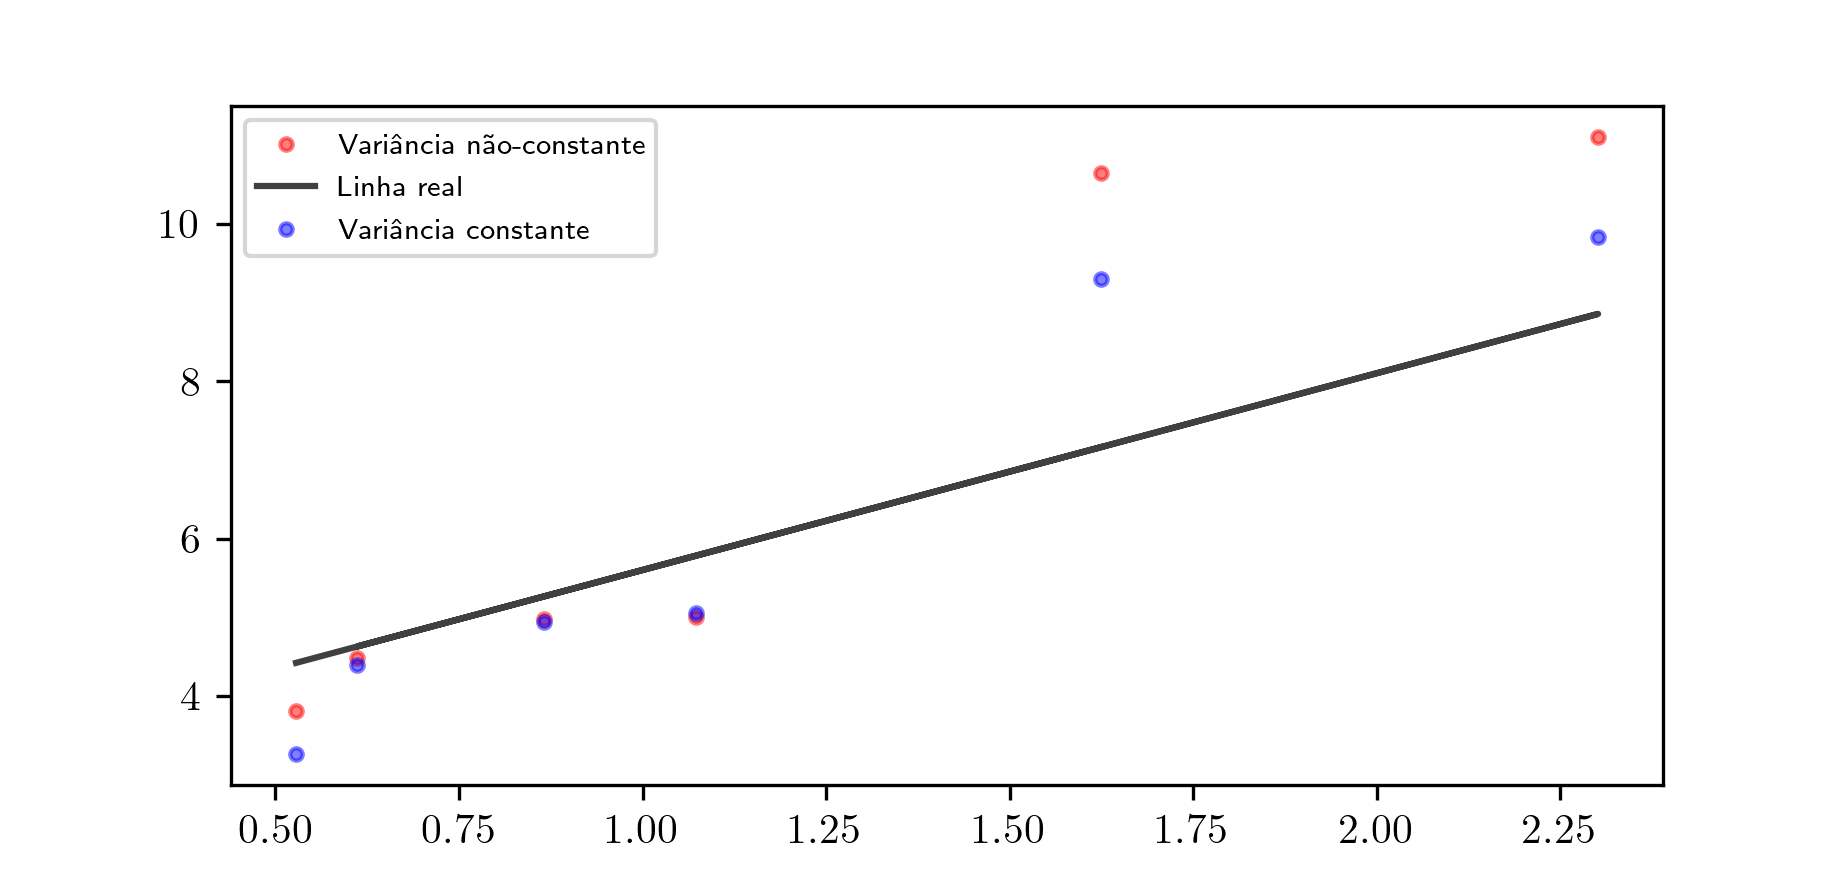
\includegraphics[width=12cm]{wls_var.png}
    \caption{Amostras com variância constante (azul) e amostras com variância não-constante (vermelho)}
    \label{fig:outlier}
\end{figure}

Em situações na qual essa premissa não é cumprida, é necessário adotar variâncias proporcionais:

\begin{equation}\label{eq:10}
Var(y_i|x_i) = \sigma^2 = \frac{1}{w_i}
\end{equation}

Onde $w_i$ são constantes de proporcionalidade, particulares a cada amostra.

De forma a utilizar deste recurso, é proposto o o método de linearização por mínimos quadrados ponderados  \cite{reg_analysis_weighted} \cite{weighted_taconeli}. Neste caso, a equação em estudo se apresenta de forma bastante semelhante ao método de mínimos quadrados ordinários, como pode ser observado na equação abaixo:

\begin{equation}\label{eq:11}
y_i = \alpha + x_i\beta +\epsilon_i^\ast
\end{equation}

Da mesma forma, $y_i$ representa o vetor de dados a serem estimados, $x_i$ representa o vetor de amostras, $\beta$ representa os coeficientes dependentes e $\alpha$ os independentes. A diferença está no $\epsilon^\ast$, que agora não mais representa erros com covariâncias constantes e sim, ao isolar $w_i$ na equação \ref{eq:10}, uma matriz de pesos denominada \textbf{W} da forma:

\begin{equation*}\textbf{W}=\left( \begin{array}{cccc} w_{1} & 0 & \ldots & 0 \\ 0& w_{2} & \ldots & 0 \\ \vdots & \vdots & \ddots & \vdots \\ 0& 0 & \ldots & w_{n} \\ \end{array} \right) \end{equation*}

Onde cada $w_i = \frac{1}{\sigma_i^2}$.

Assim, os valores de $\beta$ e $\alpha$ podem ser estimados à partir da soma dos quadrados dos erros $e_i^\ast$, da forma:

\begin{equation}\label{eq:12}
 \beta =\arg\min_{\beta}\sum_{i=1}^{n}\epsilon_{i}^{*2}\\ 
\end{equation}

Matricialmente, a equação \ref{eq:11} pode ser exposta como se segue:

\begin{equation}\label{eq:11matrix}
Y = \alpha + X\beta +\epsilon^\ast
\end{equation}

De forma um pouco mais detalhada, a equação \ref{eq:12} pode ser expandida da forma:

\begin{equation}\label{eq:13}
 S(\alpha,\beta) =\sum_{i=1}^{n} w_i(y_i - \alpha - \beta x_i)^2\\\ 
\end{equation}

Derivando como no método de mínimos quadrados ordinários, $\alpha$ e $\beta$ são equacionados:

\begin{equation}\label{eq:14}
 \alpha = \overline{y} - \beta \overline{x} 
\end{equation}

\begin{equation}\label{eq:15}
  \beta =\frac{\sum_{i=1}^{n}w_i(x_i - \overline{x})(y_i - \overline{y})}{\sum_{i=1}^{n} w_i(x_i - \overline{x})^2}\\\  
\end{equation}

Onde $\overline{x}$ e $\overline{y}$ são as médias ponderadas de \textit{x} e \textit{y}:

\begin{equation*}
  \overline{x} =\frac{\sum_{i=1}^{n}w_i x_i}{w_i}\\\  
\end{equation*}

\begin{equation*}
  \overline{y} =\frac{\sum_{i=1}^{n}w_i y_i}{w_i}\\\  
\end{equation*}

Matricialmente, representando $\textbf{X} = (x_i - \overline{x})$ e $\textbf{Y} = (y_i - \overline{y})$, a equação \ref{eq:15} é representada por:

\begin{align*} \beta =(\textbf{X}^{T}\textbf{W}\textbf{X})^{-1}\textbf{X}^{T}\textbf{W}\textbf{Y} \end{align*}

De forma gráfica, podemos comparar as duas formas de linearização por mínimos quadrados, para amostras com variância não-constante, através do exemplo exposto na figura \ref{fig:mqomqp}:

\begin{figure}[htp]
    \centering
    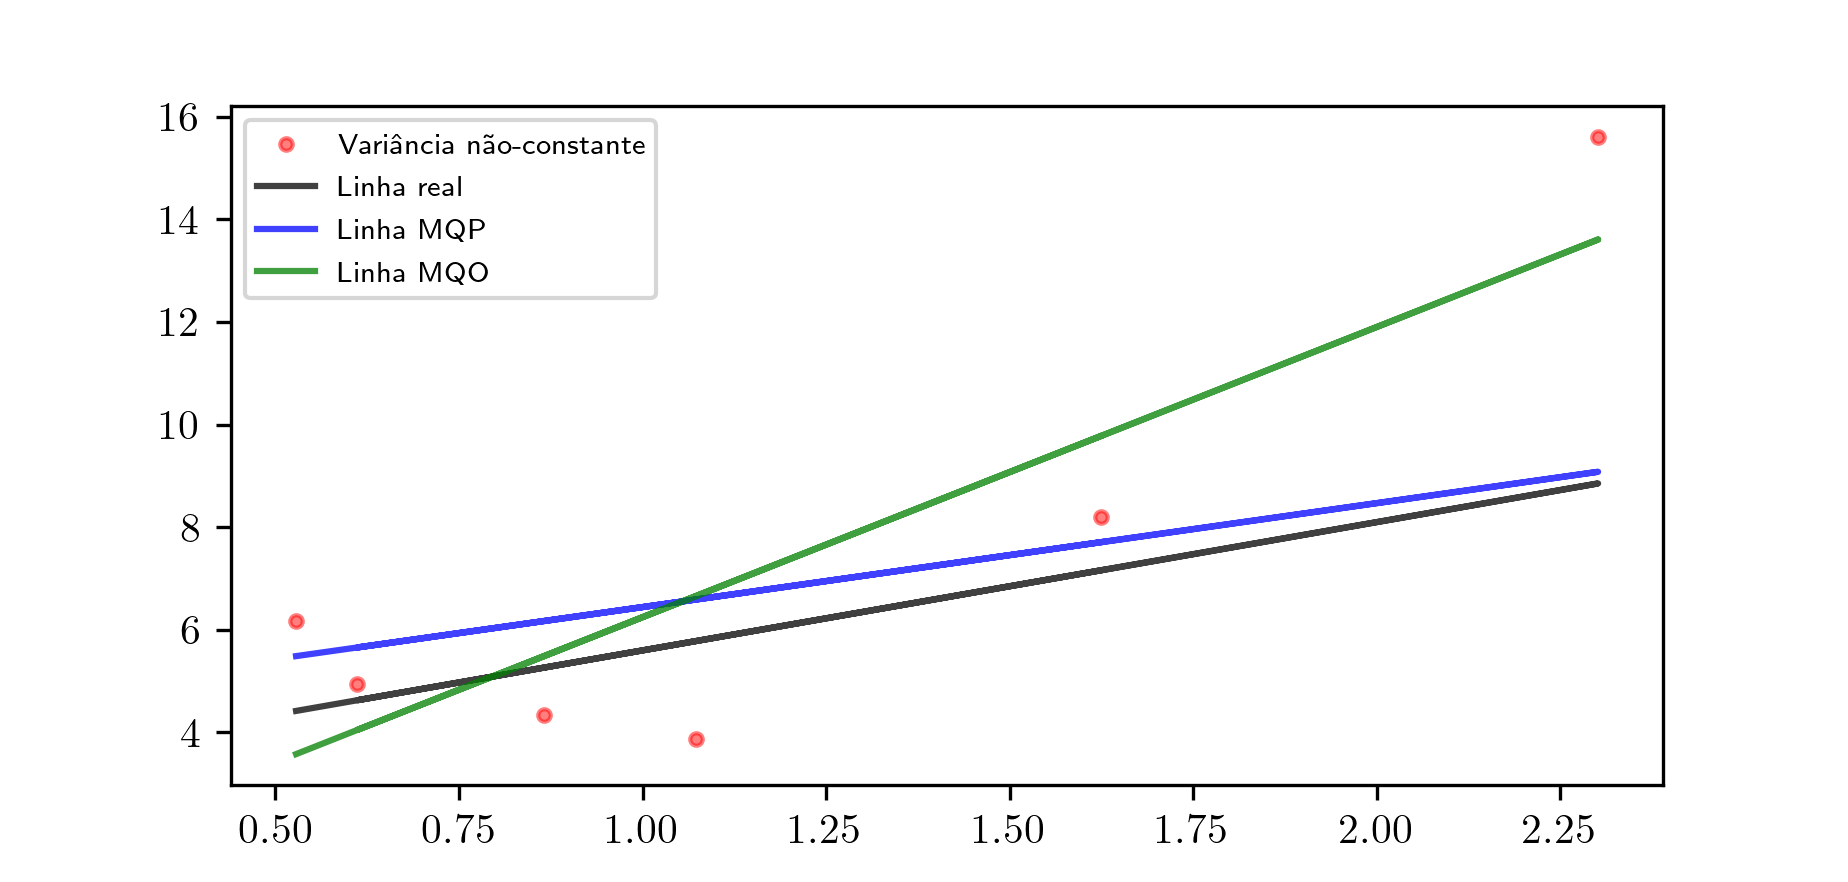
\includegraphics[width=12cm]{wls_fin.png}
    \caption{Linhas regressoras para o método dos Mínimos Quadrados Ordinários (MQO) e para o método dos Mínimos Quadrados Ponderados(MQP)}
    \label{fig:mqomqp}
\end{figure}

Como é facilmente perceptível, a linha regressora azul, referente ao resultado da linearização pelo método dos mínimos quadrados ponderados traz um erro associado significativamente menor que o observado na linha oriunda dos mínimos quadrados ordinários.

Uma das medidas de qualidade mais importantes para este tipo de regressão é o coeficiente de determinação $R^2$, que possui formulação bastante semelhante ao método de mínimos quadrados, segundo a análise de Willett e Singer \cite{r2_weighted}, diferindo apenas na soma total dos quadrados como equacionado abaixo:

\begin{equation}\label{eq:16}
R^2 = 1 - \frac{\sum_{i=1}^{n} y_i(\beta x_i + \alpha)^2}{\sum\limits_{i=1}^{n}{w_{i}y_{i}^{2}} - \frac{1}{\sum\limits_{k=1}^{n}w_{k}} \cdot \left(\sum\limits_{i=1}^{n}{w_{i}y_{i}} \right)^{2}.}
\end{equation}

Neste ponto, duas observações se fazem necessárias:

\begin{itemize}
  \item Uma vez que cada peso é inversamente proporcional à variância do erro, uma amostra com pequeno erro na variância terá um peso grande nas estimações;
  \item Os pesos deverão ser estimados (ou escolhidos arbitrariamente) considerando uma constante de proporcionalidade.
\end{itemize}

\section{Linearização por desvios mínimos absolutos - \textit{Least Absolute Deviations}}

Um dos principais pontos negativos de qualquer regressão linear por mínimos quadrados ocorre pois ao elevar ao quadrado o erro, é aumentada ao quadrado a importância das amostras com erro maior \cite{robust}. Isso pode ser particularmente prejudicial ao analisar \textit{outliers}, isto é, amostras discrepantes cujo erro pode não ter a mesma origem dos erros dos outros dados. Nestes casos, este método acabará priorizando estes valores discrepantes e isto aumentará o erro dos outros valores estimados.

Este fato é ilustrado na figura \ref{fig:infl_outlier}:

\begin{figure}[htp]
    \centering
    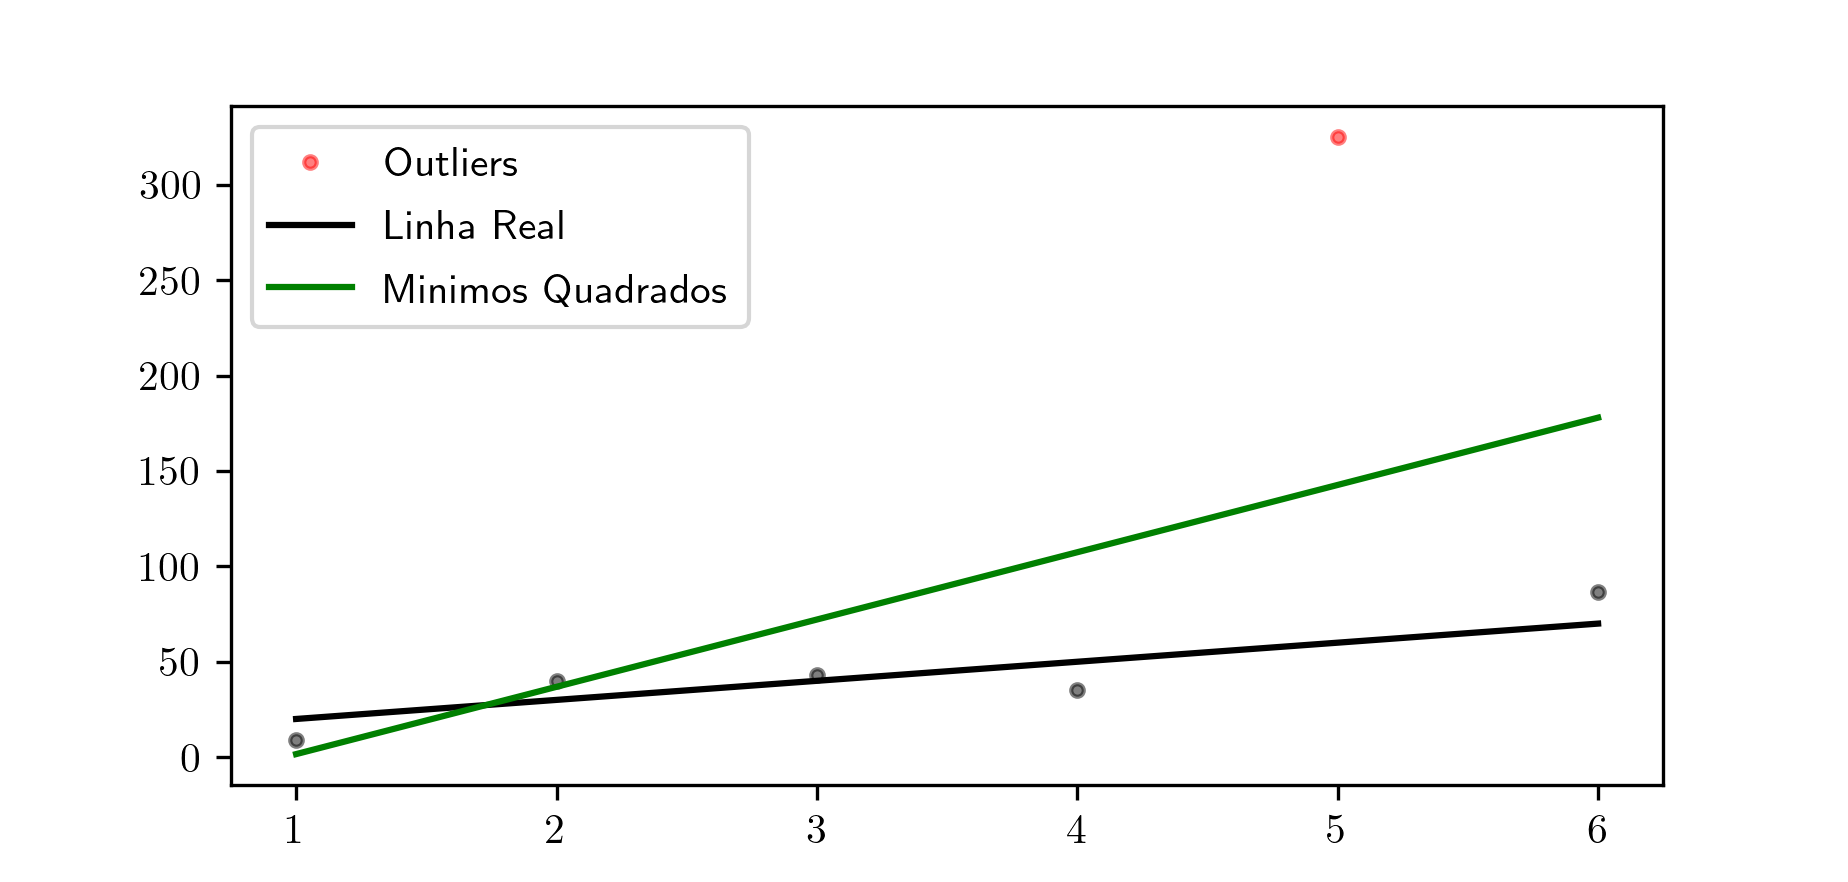
\includegraphics[width=12cm]{outlier_lsq.png}
    \caption{Influência de um \textit{outlier} na estimação dos valores de \textit{y} utilizando mínimos quadrados}
    \label{fig:infl_outlier}
\end{figure}

O \textit{outlier} (ponto em vermelho) faz com que o valor de $\beta$ aumente significativamente, inclinando a reta estimada por mínimos quadrados e aumentando o erro entre esta e os dados reais (pontos em cinza).

Visando reduzir este problema, a linearização por desvios mínimos absolutos é proposta pois a minimização neste caso é efetuada sobre o valor absoluto de $\epsilon$, em vez de $\epsilon^2$ \cite{lad}. Essa característica classifica este método de linearização como robusto \cite{robust}, isto é: mesmo que existam valores discrepantes entre as amostras, o método ainda será capaz de gerar uma solução com razoável eficiência.

Equacionando o $\beta$ para este método:

\begin{equation}\label{eq:17}
 \beta =\arg\min_{\beta}\sum_{i=1}^{n}|\epsilon_{i}|\\ 
\end{equation}

Substituindo $\epsilon$:

\begin{equation}\label{eq:18}
S(\alpha, \beta) = \sum_{i=1}^{n} |y_i - \alpha - \beta x_i|
\end{equation}

Para a implementação de um algoritmo que soluciona este método, é necessário ter em mente o fato de que a linha de regressão sempre cruza pelo menos dois pontos \cite{lad}. Tomando um primeiro ponto ($x_1$, $y_1$), deve-se buscar a melhor linha que passa através deste ponto. Esta linha deverá cruzar também outro ponto, ($x_2$, $y_2$). 

O próximo passo é procurar a melhor linha com respeito ao somatório de erros absolutos $\sum_{i=1}^{n}|\epsilon_{i}|$ que cruza ($x_2$, $y_2$). Essa linha cruzará, pelo menos, um outro ponto ($x_3$, $y_3$) e assim sucessivamente. Durante essa iterações, o valor de $\sum_{i=1}^{n}|\epsilon_{i}|$ diminui até que seja encontrada uma iteração com uma linha obtida idêntica a anterior, onde é possível concluir que esta é a melhor linha de regressão para os pontos fornecidos \cite{conciseenclyclopediaofstatistics}.

Para a construção da melhor linha cruzando ($x_1$, $y_1$), devemos encontrar o ponto ($x_k$, $y_k$) para qual a linha seja a melhor em termos de $\sum_{i=1}^{n}|\epsilon_{i}|$. Esta linha deverá ter a seguinte equação

\begin{equation}\label{eq:19}
y(x) = y_1 + \frac{y_k - y_1}{x_k - x_1} (x - x_1)
\end{equation}

Com a inclinação $\beta$:

\begin{equation}\label{eq:20}
\beta = \frac{y_k - y_1}{x_k - x_1}
\end{equation}

E com o deslocamento $\alpha$:

\begin{equation}\label{eq:21}
\alpha = y_1 - \beta x_1
\end{equation}

Para encontrar o ponto mais facilmente, são renomeados os (n - 1) pontos candidatos ${ \left(x_2,
	y_2\right), \ldots, \left(x_n,y_n\right) }$ de forma a obter:
	
\begin{equation*}
    \frac{y_2-y_1}{x_2-x_1} \leq \frac{y_3-y_1}{x_3-x_1}\leq \ldots \leq \frac{y_n-y_1}{x_n-x_1}\:
\end{equation*}

É definido também ${ T=\sum\limits_{i=1}^n \left|x_i-x_1\right| }$ para obter o ponto procurado em termos de \textit{k}, como se segue:

\begin{equation}\label{eq:22}
\begin{cases}
    \left|x_2-x_1\right| + \ldots + \left|x_{k-1}-x_1\right| & < \frac{T}{2} \\
    \begin{array}{l}\left|x_2-x_1\right| + \ldots \\+ \left|x_{k-1}-x_1\right| + \left|x_k-x_1\right|\end{array} & > \frac{T}{2}\:.
  \end{cases}
\end{equation}

Essa condição garante que $\beta$ minimize a equacão \ref{eq:23} de maneira análoga à $\sum_{i=1}^{n}|\epsilon_{i}|$ para as linhas de regressão passando por ($x_1$, $y_1$).

\begin{equation}\label{eq:23}
\sum_{i=1}^n\left| \left(y_i-y_1\right)-\beta\left(x_i-x_1\right)\right|
\end{equation}

É possível também verificar que a linha de regressão obtida passa pelo ponto ($x_k$,$y_k$), bastando apenas trocar o ponto ($x_k$,$y_k$) por ($x_2$,$y_2$) e recomeçar o algoritmo.


Utilizando os mesmos dados expostos na figura \ref{fig:infl_outlier}, a linearização por desvios mínimos absolutos traz o resultado exposto na figura \ref{fig:lad}:

\begin{figure}[H]
    \centering
    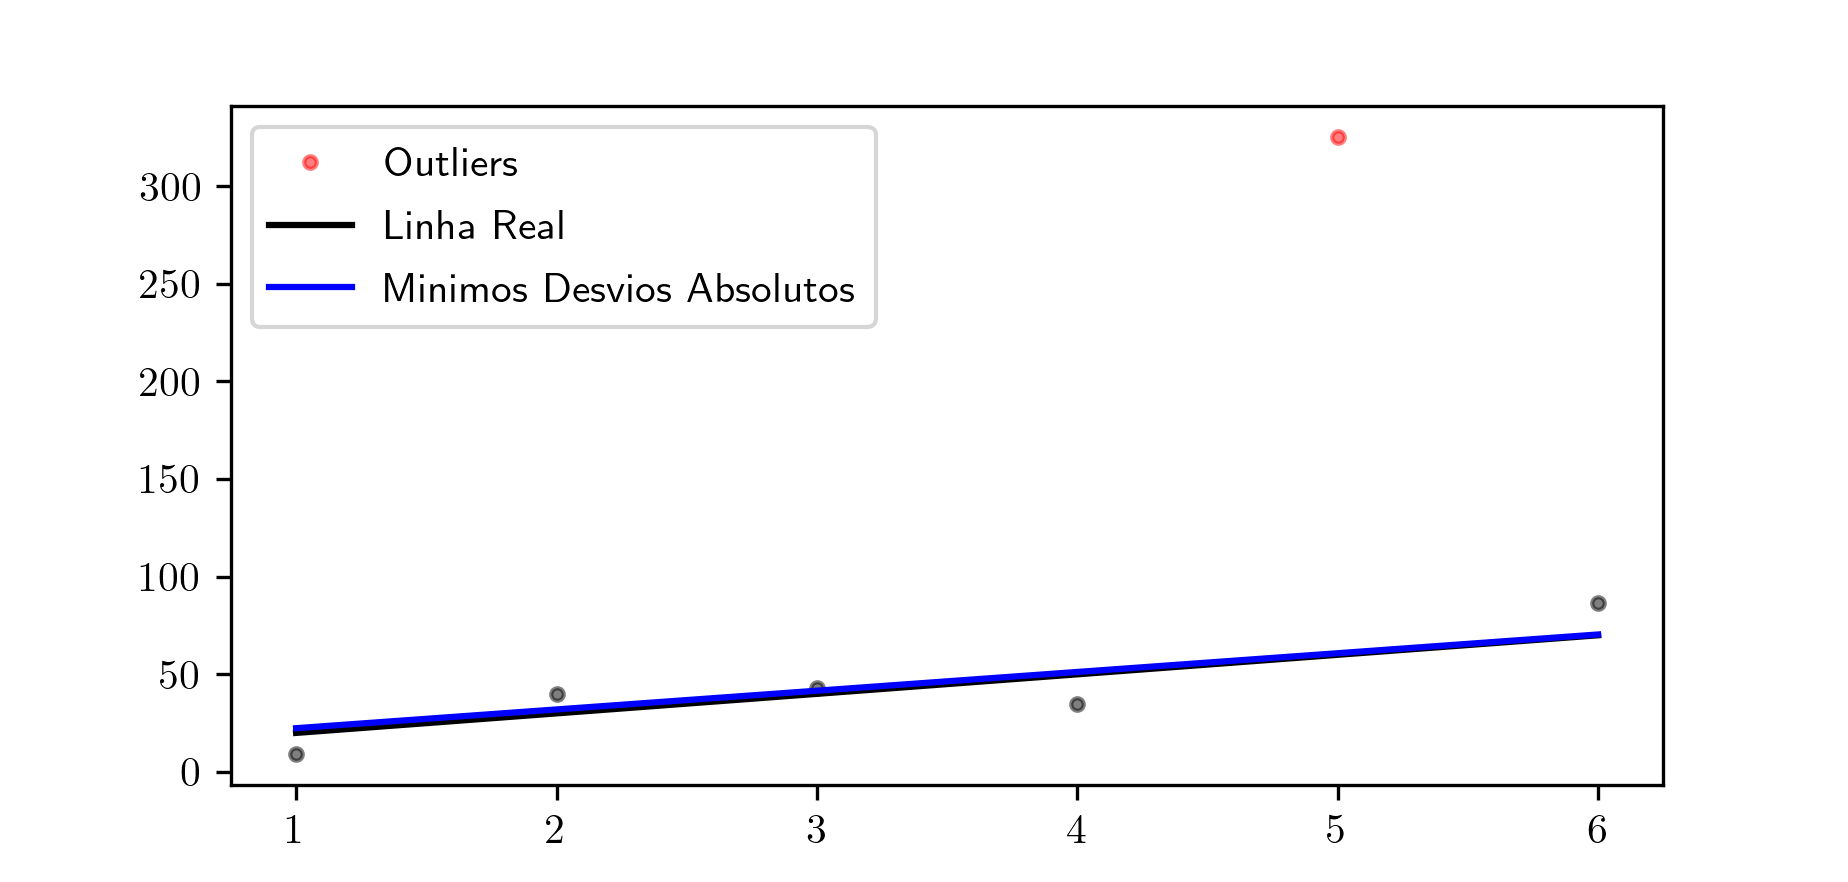
\includegraphics[width=12cm]{lad_ind.png}
    \caption{Linearização utilizando o método de desvios mínimos absolutos}
    \label{fig:lad}
\end{figure}

É facilmente observável o efeito dessa linearização: a linha de regressão estimada menospreza o \textit{outlier} em vermelho, mantendo os erros associados às outras amostras menores do que nos métodos de linearização anteriores.


Apesar destas grandes vantagens, este método possui algumas desvantagens consideráveis em relação aos anteriores, a saber:

\begin{itemize}
  \item Múltiplas soluções são possíveis;
  \item Uma ou mais soluções instáveis podem ser geradas pelo método. Isto é: a solução obtida poderá, para um pequeno ajuste no eixo \textit{y}, modificar a linha de regressão enormemente \cite{instabilitylad};
  \item Por ser um método essencialmente iterativo desde a estimação dos valores iniciais, uma maior quantidade de recursos computacionais se faz necessária.
\end{itemize}


    % Capitulo de revisão de literatura
    
% The \phantomsection command is needed to create a link to a place in the document that is not a
% figure, equation, table, section, subsection, chapter, etc.
% https://tex.stackexchange.com/questions/44088/when-do-i-need-to-invoke-phantomsection
\phantomsection

% Multiple-language document - babel - selectlanguage vs begin/end{otherlanguage}
% https://tex.stackexchange.com/questions/36526/multiple-language-document-babel-selectlanguage-vs-begin-endotherlanguage
\begin{otherlanguage*}{brazil}

\chapter{Metodologia}

  %  \begin{flushright}
 %       \englishword{\showfont}
 %  \end{flushright}
\label{cap_metodologia}

\section{Ambiente de testes} %Ambiente
% Topologia de testes geral para a subestação e também a minha proposta (usada na proposta de TCC)
% Detalhes dos protocolos estilo el
%olhar posição da legenda nas imagens

Para a implementação das metodologias de testes utilizadas neste trabalho, foi necessário reproduzir em laboratório o ambiente de utilização real de uma \textit{Merging Unit}, isto é: foi necessário reproduzir o ambiente da subestação elétrica digital no qual o equipamento está inserido. O esquema exposto na figura \ref{fig:diag_substation} ilustra como é este sistema:

\begin{figure}[H]
    \centering
    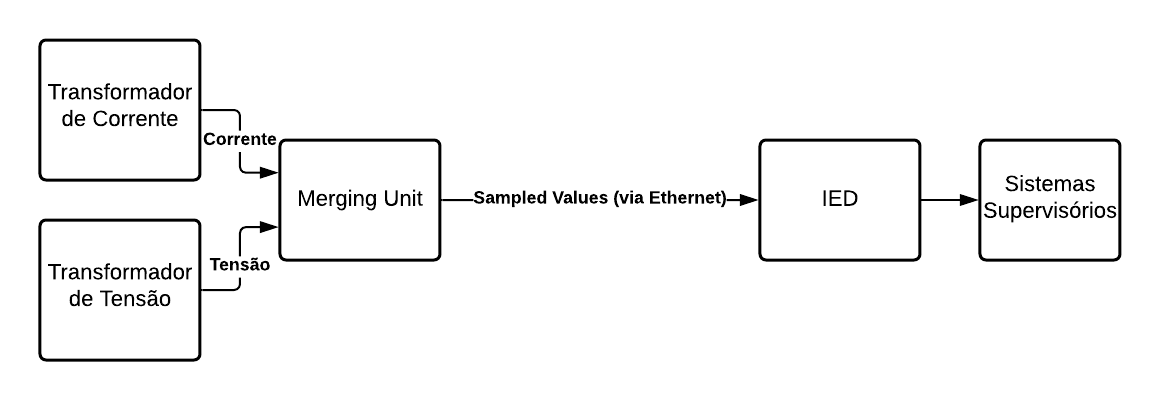
\includegraphics[width=12cm]{pictures/diag_substation_tcc.png}
    \caption{Exemplo de utilização de uma \textit{Merging Unit} em uma subestação elétrica digital}
    \label{fig:diag_substation}
\end{figure}

Neste exemplo, a \textit{Merging Unit} serve como interface entre os transformadores de instrumentação e os IEDs da rede, gerando o fluxo de \textit{Sampled Values} conforme com a norma IEC-61850 \cite{IEC61850_7-2} à partir dos sinais de corrente e tensão aplicados. IED, do inglês \textit{Intelligent Electronic Device} ou Dispositivo Eletrônico Inteligente, é qualquer dispositivo que incorpora um ou mais processadores com a capacidade de receber ou enviar/controlar dados de ou para uma fonte externa de sinal (e.g., relés digitais, disjuntores) \cite{substation_basics}. Já \textit{Sampled Values} \cite{sv_typhoonhil} é o protocolo padrão utilizado para comunicação ente as \textit{Merging Units} e os IEDs. Este protocolo é do tipo \textit{publisher/subscriber}, onde o \textit{publisher} (neste caso a \textit{Merging Unit}), envia mensagens pela rede \textit{Ethernet} periodicamente com intervalos de tempo precisamente definidos. Estas mensagens contém o valor amostrado de cada um dos sinais aplicados nas placas de aquisição analógica da \textit{Merging Unit}. O intervalo de tempo depende de dois fatores: a frequência do sinal medido e a quantidade de amostras por ciclo de sinal. A norma IEC 61850-9-2LE \cite{IEC61850_7-2} define dois valores para a quantidade de amostras por ciclo: 80 para equipamentos de proteção e 256 para equipamentos de medição. Para a frequência do sinal adquirido não há restrições, sendo 50 e 60 Hz os valores mais comumente utilizados. O \textit{subscriber}, representado neste exemplo pelos \textit{IEDs}, ``subscreve'' aos pacotes de \textit{Sampled Values} buscando receber informações sobre um determinado dispositivo da rede.

Para reproduzir esse mesmo ambiente em laboratório, são substituídos os transformadores por uma fonte de tensão e corrente e o IED por um computador, que receberá e processará os \textit{Sampled Values}. A imagem \ref{fig:met_acq} ilustra esse ambiente:

\begin{figure}
    \centering
    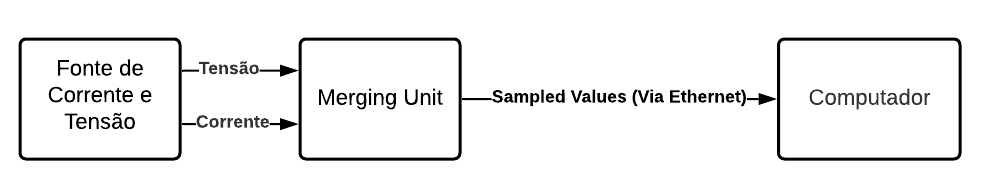
\includegraphics[width=12cm]{pictures/met_acq.png}
    \caption{Ambiente em laboratório para aquisição de dados com \textit{Merging Unit}}
    \label{fig:met_acq}
\end{figure}

Após a aquisição dos \textit{Sampled Values} pelo computador via interface de rede \textit{Ethernet}, se faz necessária a conversão deste fluxo de dados em um formato padrão para oscilografias em sistemas elétricos. Para tanto, é escolhido o formato COMTRADE \cite{comtrade1992} \cite{C37.111-2013}, que é o acrônimo para \textit{Common Format for Transient Data Exchange}, ou Formato Comum para Troca de Dados Transientes. Este formato é composto, no mínimo, por dois arquivos: um arquivo de configuração com extensão .cfg, que descreve os canais de aquisição contidos no COMTRADE e suas características, como frequência nominal do canal, quantidade de canais amostrados, unidade de medição, etc. O quadro \ref{quad:quadro_confcomtra} ilustra um exemplo de arquivo de arquivo de configuração de COMTRADE.

\begin{quadro}[htb]
\caption[Exemplo do arquivo de configuração do COMTRADE]{Exemplo do arquivo de configuração do COMTRADE.}
\label{quad:quadro_confcomtra}
\begin{tabular}{|l|}
%\hline
Test,518,1999 <CR/LF>\\
12,6A,6D <CR/LF>\\
1,P Va-g,,,kV, 0.14462,0.0000000000,0,–2048,2047,2000,1,P <CR/LF>\\
2,P Vc-g,,,kV, 0.14462,0.0000000000,0,–2048,2047,2000,1,P <CR/LF>\\
3,P Vb-g,,,KV, 0.14462,0.0000000000,0,–2048,2047,2000,1,P <CR/LF>\\
4,P Ia,,,A,11.5093049423,0.0000000000,0,–2048,2047,1200,5,P <CR/LF>\\
5,P Ib,,,A,11.5093049423,0.0000000000,0,–2048,2047,1200,5,P <CR/LF>\\
6,P Ic,,,A,11.5093049423,0.0000000000,0,–2048,2047,1200,5,P <CR/LF>\\
1,Va over,,,0 <CR/LF>\\
2,Vb over,,,0 <CR/LF>\\
3,Vc over,,,0 <CR/LF>\\
4,Ia over,,,0 <CR/LF>\\
5,Ib over,,,0 <CR/LF>\\
6,Ic over,,,0 <CR/LF>\\
60 <CR/LF>\\
1 <CR/LF>\\
6000.000,885 <CR/LF>\\
20/07/2005,17:38:26.663700 <CR/LF>\\
20/07/2005,17:38:26.687500 <CR/LF>\\
ASCII <CR/LF>\\
1\\
\hline
\end{tabular}
%\fonte{Teste. -- \showfont}
\end{quadro}

O outro arquivo imprescindível para o COMTRADE é o que contém as próprias amostras, com extensão .dat. Este arquivo pode estar codificado em ASCII com representação decimal separada por vírgulas ou em binário. Os arquivos em ASCII e em binário possuem estrutura idêntica por linha, contendo o número da amostra, o intervalo de tempo em relação ao início do registro em $\mu s$, as medidas analógicas e também as digitais. No modo binário, as informações numéricas estão em formato \textit{little-endian} de 16 bits, enquanto no formato ASCII estas são separadas por vírgula e por uma quebra de linha ao final de cada amostra. O quadro \ref{quad:quadro_dat1comtra} exemplifica essa estrutura.


\begin{quadro}[htb]
\caption[Exemplo de uma linha do arquivo de dados do COMTRADE]{Exemplo de uma linha do arquivo de dados do COMTRADE.}
\label{quad:quadro_dat1comtra}
\centering
\begin{tabular}{|c|}
%\hline
5, 667, –760, 1274, 72, 61, –140, –502,0,0,0,0,1,1 <CR/LF>\\
\hline
\end{tabular}
%\fonte{Teste. -- \showfont}
\end{quadro}


\section{Geração de Sinais e Aquisição pela \textit{Merging Unit}}

%Para capturar os dados necessários para a aplicações dos algoritmos de calibração, se faz necessária a montagem de uma configuração de testes capaz de aplicar sinais previamente programados e com precisão adequada nos canais de tensão e corrente das placas de aquisição analógica da \textit{Merging Unit}. Estes sinais serão condicionados pelo circuito de  instrumentação de entrada da placa e, posteriormente, serão transformados em um fluxo de dados segundo o protocolo \textit{Sampled Values}, conforme a norma IEC-61850 \cite{IEC61850_7-2}, para posteriormente serem capturados por um computador. Este protocolo é usado para a troca de informações entre a \textit{Merging Unit} e os \textit{IEDs - Intelligent Electronic Devices}, ou Dispositivos Eletrônicos Inteligentes, em uma subestação elétrica digital com rede \textit{Ethernet} \cite{sv_typhoonhil}. Um \textit{IED} é qualquer dispositivo que incorpora um ou mais processadores com a capacidade de receber ou enviar/controlar dados de ou para uma fonte externa de sinal (e.g., relés digitais, disjuntores) \cite{substation_basics}.

Na configuração de testes proposta, será utilizada uma fonte de sinais de tensão e corrente programável com precisão maior que as placas de aquisição analógica da \textit{Merging Unit} em análise, de forma a reduzir os erros inerentes ao  sinal aplicado. À partir destes sinais, a \textit{Merging Unit} deverá capturar e processar em tempo real gerando como saída um fluxo de \textit{Sampled Values}. Estes fluxo de dados deverá ser direcionado a um computador para processamento posterior via interface de rede \textit{ethernet}.

\section{Recebimento dos Pacotes de \textit{Sampled Values} e reconstrução dos sinais aplicados}

Já com estes pacotes de \textit{Sampled Values} recebidos pelo computador, é momento de processar esses dados de forma a poder discernir e reconstruir os sinais para cada um dos canais de aquisição analógica da \textit{Merging Unit}. O primeiro passo deste processamento é a conversão desses pacotes em COMTRADEs. Através deste formato, cada uma das amostras presentes nos dados gerados pela \textit{Merging Unit} torna-se um valor numérico de corrente ou tensão, permitindo representar os sinais aplicados pela fonte de tensão e corrente. Na figura \ref{fig:sig_corr_reconst}, é observada essa reconstrução de um sinal de corrente de 50mA RMS:

\begin{figure}[H]
    \centering
    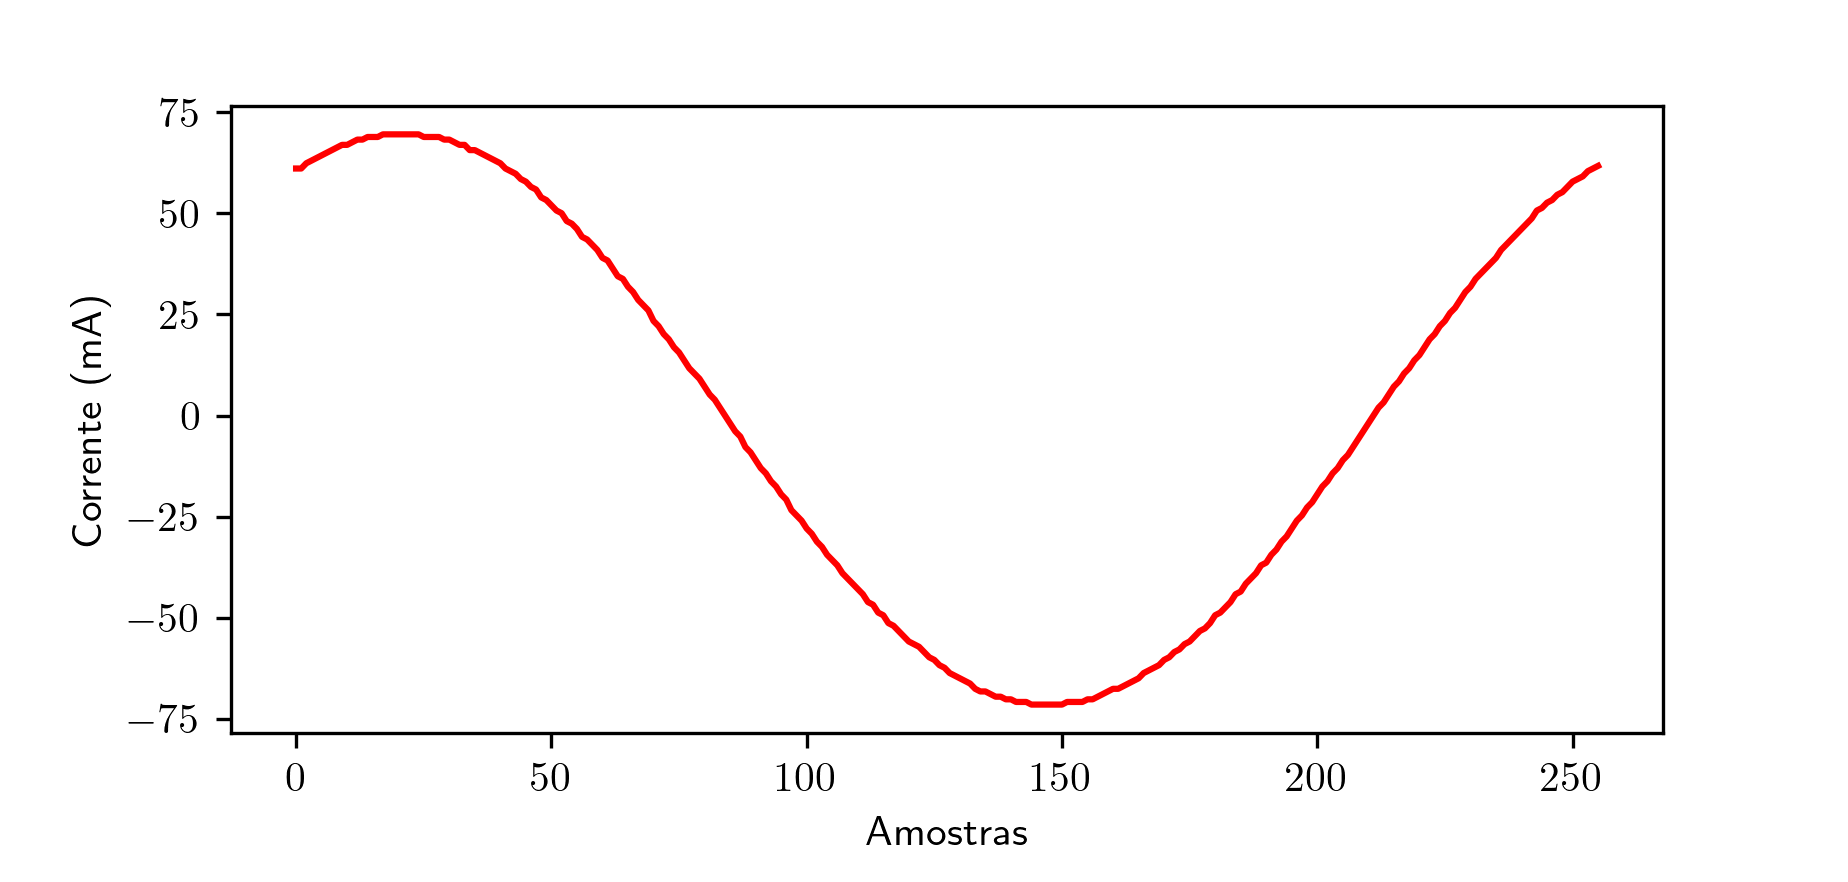
\includegraphics[width=14cm]{pictures/sig_corr_reconst.png}
    \caption{Exemplo de oscilografia construída à partir de COMTRADE.}
    \label{fig:sig_corr_reconst}
\end{figure}

\section{Cálculo dos erros de magnitude e análise da fase e da frequência dos sinais reconstruídos}

Após a reconstrução das amostras para cada um dos canais de aquisição, é calculado o valor quadrático médio ou RMS (do inglês \textit{Root Mean Square}) por ciclo, como exposto na equação \ref{eq:24}:

\begin{equation}\label{eq:24}
RMS(k) = \sqrt{\frac{1}{N} \sum_{i=0}^{N - 1} |u(Nk + i)|^2}
\end{equation} 

Onde N representa o número de amostras por ciclo do sinal avaliado e k é o índice que representa o ciclo atual do sinal. A função $u(Nk + i)$ representa os sinais amostrados de corrente e tensão em análise.

Estes valores são muito informativos pois restringem o múmero de amostras utilizadas como entrada para os algoritmos de calibração de cada canal, sem perder informações substanciais dos sinais originais. 

Neste ponto, é possível calcular os erros de magnitude entre o valor RMS dos sinais aplicados pela fonte e cada um dos valores RMS obtidos por ciclo. De forma a aumentar a variedade dos resultados e trazer mais informações, para cada sinal aplicado são salvos o maior, o menor e a média entre os erros. 

Apesar de não haver sincronismo entre os sinais aplicados pela fonte, isto é, não é sabida a fase inicial destes sinais, é possível ainda assim avaliar eventuais distorções de fase comparando a o sinal obtido à partir do COMTRADE com um sinal senoidal/cossenoidal ideal sem defasamento inicial. Na prática, é possível obter o defasamento inicial através do seguinte procedimento \cite{understandingdsp}: considerando um triângulo retângulo no qual o ângulo será igual ao ângulo de defasamento inicial do sinal, o cateto adjacente será obtido através do produto interno entre as amostras do sinal com fase desconhecida e as amostras do seno ideal, e o cateto oposto será obtido ao efetuar a mesma operação entre as amostras do sinal real e o cosseno ideal. Para conseguir o defasamento, basta obter o arco tangente do quociente entre o resultado dos dois produtos internos. 

Para obter a frequência dos sinais reconstruídos à partir dos COMTRADEs, de forma a poder comparar com a frequência dos sinais gerados pela fonte, é calculada a Transformada Discreta de Fourier (do inglês \textit{Discrete Fourier Transform} ou DFT) do sinal, levando o sinal do domínio do tempo para o domínio da frequência e observando o espectro resultante, onde os pontos diferentes de zero representam as frequências presentes no sinal \cite{lathisig}. O resultado desde procedimento é ilustrado no gráfico da figura \ref{fig:dft_freq}, para um sinal com frequência de 60Hz:

\begin{figure}[H]
    \centering
    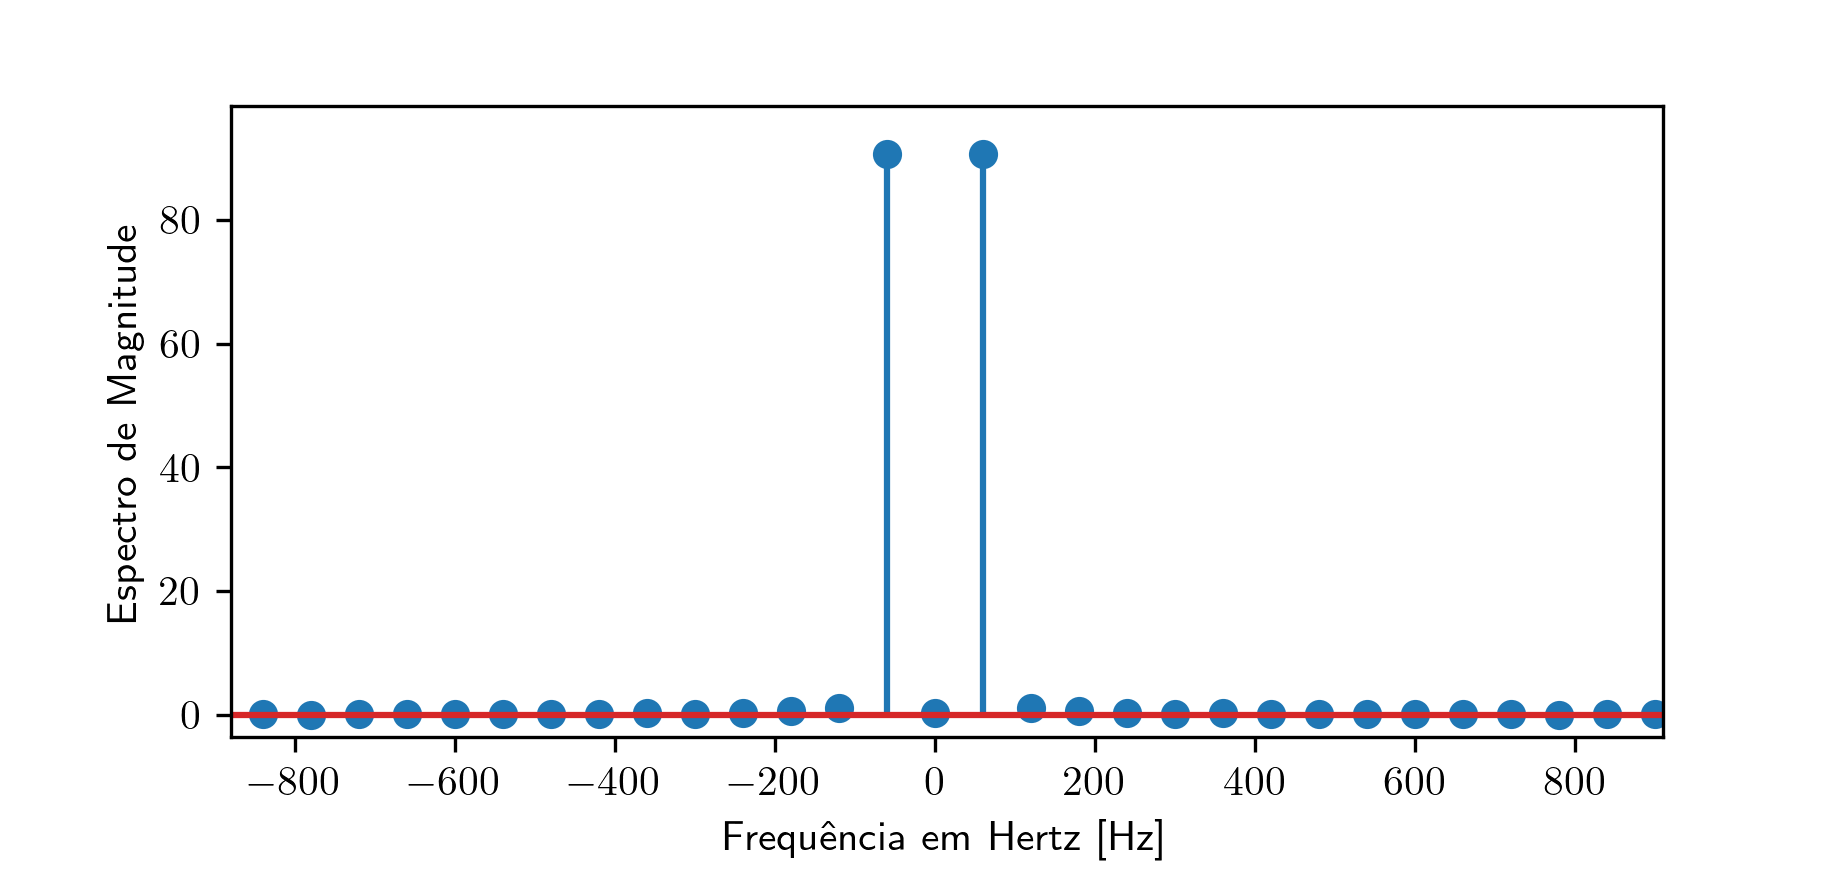
\includegraphics[width=14cm]{pictures/spec_mag.png}
    \caption{Exemplo de espectro de magnitude resultante do cálculo da DFT, a fim de encontrar a frequência do sinal.}
    \label{fig:dft_freq}
\end{figure}

\section{Aplicação dos Métodos de Calibração e avaliação dos Resultados}

Para obter os valores de entrada para os métodos de calibração  descritos no capítulo \ref{cap_algoritmos}, são analisados os valores RMS para cada ciclo de medição e escolhidos os valores que possuam maior erro de magnitude em relação ao valor de referência aplicado pela fonte de tensão e corrente. De forma a ampliar os resultados, também serão utilizados como valores de entrada os valores RMS que possuam o menor erro em relação ao valor de referência e também a média entre os valores RMS de cada ciclo de sinal aplicado.

Com estes valores em mãos, faz-se mister a aplicação destes nos algoritmos, obtendo assim os coeficientes $\alpha$ e $\beta$ de linearização para cada um dos métodos. Estes coeficientes são então aplicados nos valores de entrada, com o intuito de verificar o impacto da calibração dos canais de aquisição sobre os sinais de tensão e corrente amostrados.

A fim de encontrar o melhor entre os algoritmos propostos, são analisados os novos erros de magnitude entre os sinais aplicados pela fonte e os sinais calibrados, bem como figuras de mérito inerentes a este tipo de linearização, como o coeficiente de determinação $R^2$. 

Com o resultado desta análise, é então possível avaliar qual das metodologias de calibração para os canais de aquisição analógica da \textit{Merging Unit} trouxe melhores resultados, isto é: qual reduziu mais os seus erros em relação ao sinal aplicado.

De forma a sumarizar os processos descritos nesta seção, a figura \ref{fig:diag_met_aval} ilustra cada um dos passos acima descritos.

\begin{figure}[H]
    \centering
    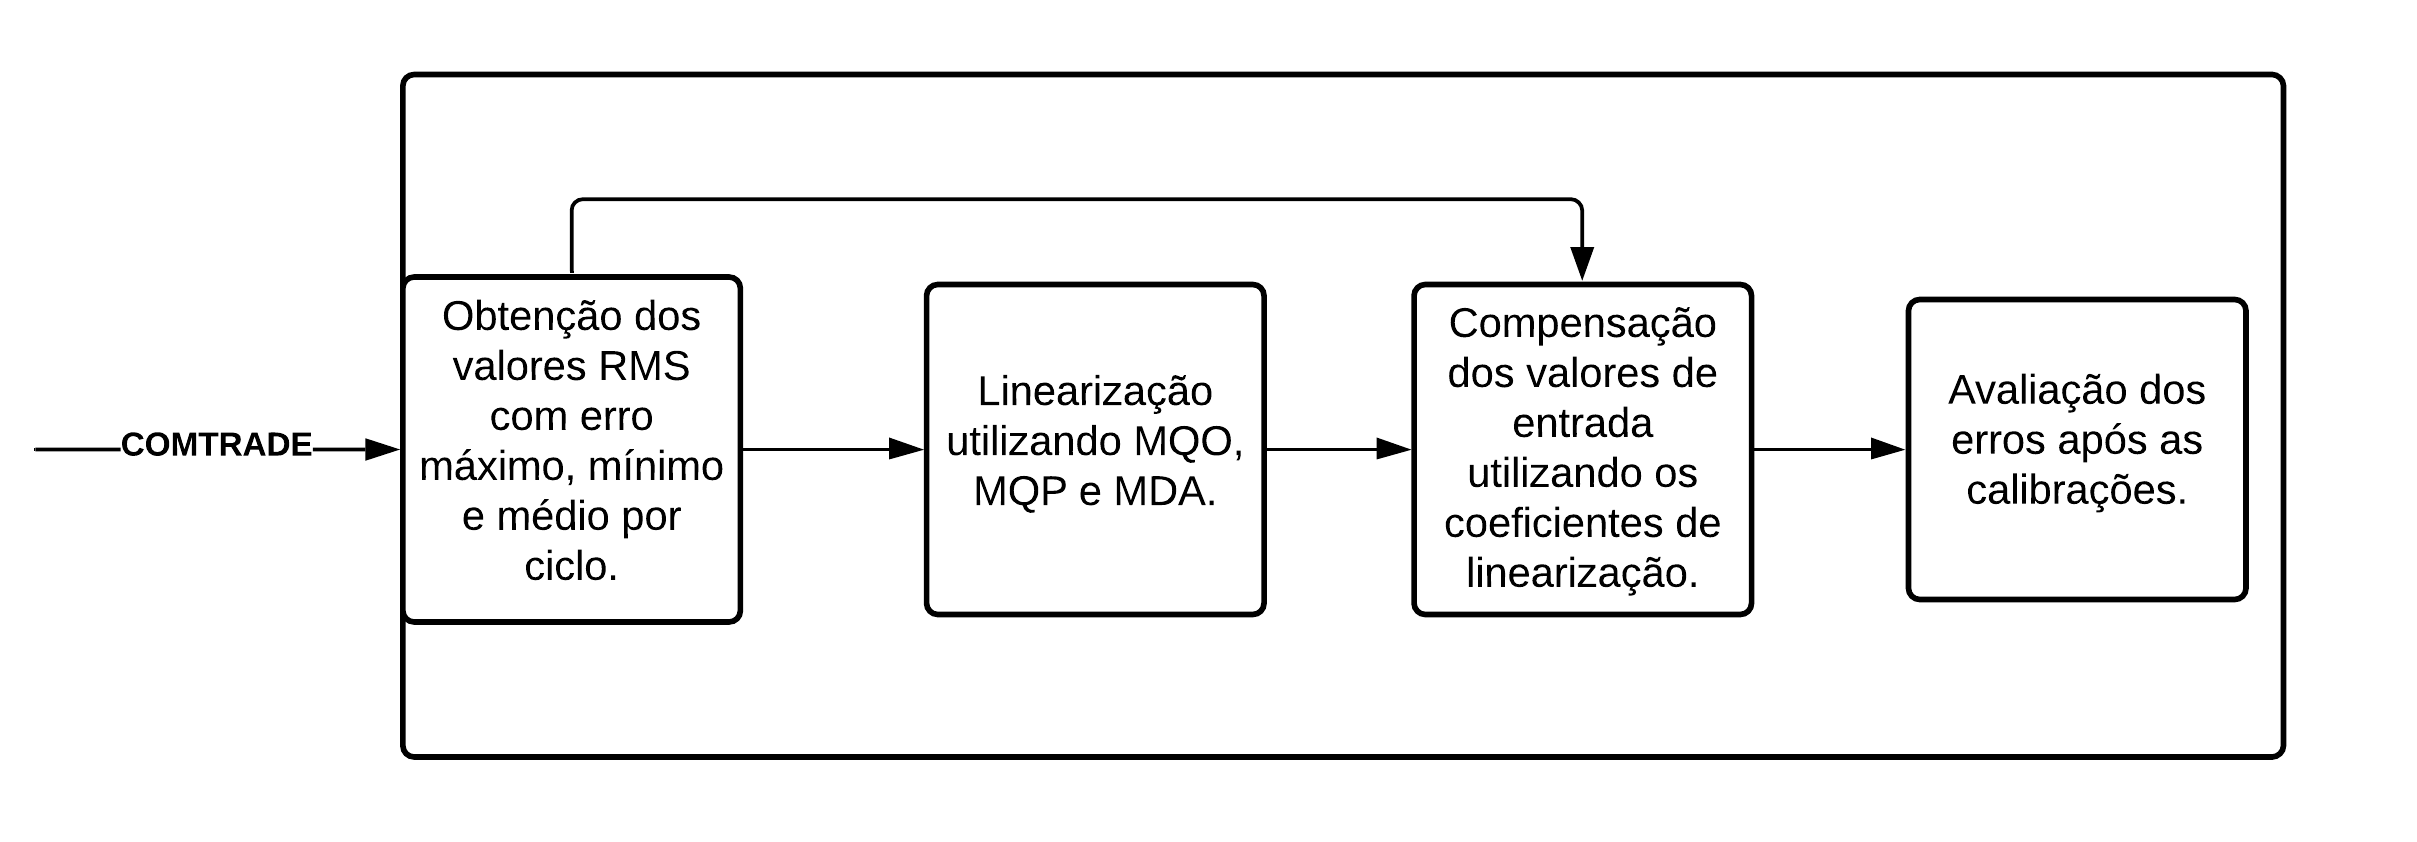
\includegraphics[width=14cm]{pictures/diag_met_avalia.png}
    \caption{Diagrama dos procedimentos descritos na seção de aplicação dos métodos de calibração e avalia os resultados.}
    \label{fig:diag_met_aval}
\end{figure}

\end{otherlanguage*}



    % Primeiro capitulo de Resultados
    
% The \phantomsection command is needed to create a link to a place in the document that is not a
% figure, equation, table, section, subsection, chapter, etc.
% https://tex.stackexchange.com/questions/44088/when-do-i-need-to-invoke-phantomsection
\phantomsection

% Multiple-language document - babel - selectlanguage vs begin/end{otherlanguage}
% https://tex.stackexchange.com/questions/36526/multiple-language-document-babel-selectlanguage-vs-begin-endotherlanguage


\chapter{Resultados}
\label{cap_resultados}
%\renewcommand{\topfraction}{.75}
%\renewcommand{\floatpagefraction}{.95}
%\renewcommand{\textfraction}{.75}

Utilizando a metodologia descrita no \autoref{cap_metodologia}, foram executadas uma série de ensiaios de aquisição, transmissão e processamento de dados utilizando uma \textit{Merging Unit} comercial com o intuito de validar os métodos propostos no \autoref{cap_algoritmos}. 

\section{Equipamentos Utilizados}

O equipamento utilizado como fonte de tensão e corrente foi a fonte de referência \textit{Fluke 6100A} \cite{fluke6100a}. Este dispositivo é amplamente utilizado para a calibração de equipamentos de medição presentes em sistemas de energia elétrica, sendo assim a fonte ideal para estes ensaios.

A \textit{Merging Unit} utilizada nos ensaios possui três tipos de placas de aquisição analógica: duas de proteção, com 1A e 5A de correntes de entrada nominais, e uma de medição, com 1A de corrente nominal. Nos ensaios descritos neste capítulo, foi utilizada uma placa de aquisição deste terceiro modelo, por conta de ser a placa que possui especificações de precisão mais rígidas. Todos os três modelos possuem 115V de tensão nominal, 50/60Hz de frequência nominal e oito canais de aquisição, sendo quatro de corrente e quatro de tensão. Na tabela \ref{tab:specsMEA} estão descritas as especificações de precisão de corrente desta placa e na tabela \ref{tab:specsMEV} as especificações de tensão.

\begin{table}[H]
\IBGEtab{
  \caption[Especificações de Corrente de entrada para a placa de aquisição utilizada.]{Especificações de Corrente de entrada para a placa de aquisição utilizada.}
  \label{tab:specsMEA}
}{%
  \begin{tabular}{ccc}
  \toprule
   \textbf{Faixa de amplitude (A)} & \textbf{Erro} & \textbf{Erro de Fase} \\
  \midrule
   0.05In ... 0.2In       & < 0.6 \% rd     & < $\pm$ $0.3^{\circ}$  \\
  \midrule
   0.2In ... 0.8In        & < $\pm$ 0.2 \%  rd & < $\pm$ $0.15^{\circ}$  \\
  \midrule
  0.8In ... 4In           & < $\pm$ 0.1 \% rd & < $\pm$ $0.1^{\circ}$ \\
  \midrule
  4In ... 40In           & < $\pm$ 0.4 \%  rd & < $\pm$ $0.2^{\circ}$ \\
  \bottomrule
\end{tabular}
}{
  \fonte{Produzido pelo autor.}
  \nota{rd representa o valor lido (em A).}
 % regressão linear. -- \showfont}%
  %\nota[Anotações]{Uma anotação adicional, que pode ser seguida de várias
  %outras. -- \showfont}%
  }
\end{table}


\begin{table}[H]
\IBGEtab{%
  \caption[Especificações de Tensão de entrada para a placa de aquisição utilizada.]{Especificações de Tensão de entrada para a placa de aquisição utilizada.}%
  \label{tab:specsMEV}
}{%
  \begin{tabular}{ccc}
  \toprule
   \textbf{Faixa de amplitude (V)} & \textbf{Erro} & \textbf{Erro de Fase} \\
  \midrule
   0.08Vn ... 2Vn       & < 0.1\% rd     & < $\pm$ $0.1^{\circ}$  \\
  \bottomrule
\end{tabular}%
}{%
  \fonte{Produzido pelo autor.}%
  \nota{rd representa o valor lido (em V).}
  %\nota{Esta é uma nota, que diz que os dados são baseados na
 % regressão linear. -- \showfont}%
  %\nota[Anotações]{Uma anotação adicional, que pode ser seguida de várias
  %outras. -- \showfont}%
  }
\end{table}

Por serem de medição, os sinais aplicados nas entradas desta placa são amostrados 256 vezes por ciclo, trazendo 15360 amostras por segundo.

A \textit{Merging Unit} escolhida para estes experimentos possui apenas dois parâmetros de calibração: ganho e \textit{offset}. Isso vale dizer que, na prática, é possível apenas calibrar estas placas de aquisição com linearizações de primeira ordem.

\section{Sinais Aplicados}

Com o intuito de cobrir o máximo das faixas de aquisição do equipamento, os ensaios foram efetuados aplicando os seguintes sinais, cada qual com a duração de 2s:

\begin{itemize}
    \item 9.2V e 0.05A (8\% da tensão nominal e 5\% da corrente nominal);
    \item 57V e 0.2A (49\% da tensão nominal e 20\% da corrente nominal);
    \item 92V e 1A (80\% da tensão nominal e 100\% da corrente nominal);
    \item 115V e 1.2A (100\% da tensão nominal e 120\% da corrente nominal);
    \item 138V e 3A (120\% da tensão nominal e 300\% da corrente nominal);
    \item 161V e 4A (140\% da tensão nominal e 400\% da corrente nominal).
\end{itemize}

Estes ensaios foram executados para as frequências de 50Hz e 60Hz. Apesar das especificações da \textit{Merging Unit} utilizada não trazer informações sobre os erros relacionados à frequência do sinal amostrado, esta variedade de frequências foi utilizada pois na norma que define os requisitos para as \textit{Merging Units} \cite{IEC61869-13}, há uma série de especificações e restrições em termos de frequência do sinal aplicado.

\section{Erros antes das calibrações}

A fim de expor os erros antes das calibrações de maneira objetiva, mas que contenham a quantidade necessária detalhes necessária para a análise antes e após a aplicação dos métodos de calibração, foram escolhidos um canal de tensão e um de corrente. De forma puramente arbitrária, foram escolhidos o canal VC de tensão e o canal IA de corrente.

As tabelas \ref{tab:tabelaerros60A} e \ref{tab:tabelaerros60V} mostram os erros máximos, mínimos e médios entre os valores aplicados pela fonte de referência em 60Hz nos canais de corrente IA e de tensão VC e o sinal obtido a partir do fluxo de dados (registro no formato COMTRADE) gerado pela \textit{Merging Unit} antes de qualquer calibração. 

\begin{table}[H]
\IBGEtab{%
  \caption[Sinais de corrente em 60Hz aplicados do canal de corrente IA e os erros observados no COMTRADE gerado]{Sinais de corrente em 60Hz aplicados do canal de corrente IA e os erros observados no COMTRADE gerado.}%
  \label{tab:tabelaerros60A}
}{%
\begin{tabular}{cccccccc}
  %\small -> diminuir fonte
  \toprule
   \textbf{Canal IA} &  & &  \\
  \midrule
  \textbf{Val. Apl. (mA)} & \textbf{Err. Máx.} & \textbf{Valor Máx.} & \textbf{\%} & \textbf{Valor Mín.} & \textbf{\%} & \textbf{Valor Méd.} & \textbf{\%}  \\
  \midrule
  50 & 0.6 \% & 49.6972 & -0.6054 & 50.0724 &  0.1449 & 49.9492 & -0.1015 \\
  \midrule
  200  & 0.2 \% &198.4886 &	-0.7557 &	198.8362 &	-0.5819	 & 198.6554 &-0.6723   \\
  \midrule
  1000 & 0.1 \% & 992.5441 &	-0.7456 & 996.3666 & -0.3633 & 994.4909 & -0.5509 \\
  \midrule
  1200 & 0.1 \% & 1191.3389 & -0.7218 & 1195.8324 & -0.3473 &	1193.9886 &	-0.501 \\
  \midrule
  3000 & 0.1 \% & 2977.7406 &	-0.7427	& 2986.4467 & -0.4518 & 2980.7856 & -0.6405 \\
  \midrule
  4000 & 0.1 \% & 3970.6934 &	-0.7327	& 3984.9192 & -0.377 & 3976.2538 & -0.5937 \\
  \bottomrule
\end{tabular}%
}{%
  \fonte{Produzido pelo autor.}%
 % \nota{rd representa o valor lido (em V).}
  %\nota{Esta é uma nota, que diz que os dados são baseados na
 % regressão linear. -- \showfont}%
  %\nota[Anotações]{Uma anotação adicional, que pode ser seguida de várias
  %outras. -- \showfont}%
  }
\end{table}

\begin{table}[H]
\IBGEtab{%
  \caption[Sinais de tensão em 60Hz aplicados do canal de tensão VC e os erros observados no COMTRADE gerado]{Sinais de tensão em 60Hz aplicados do canal de tensão VC e os erros observados no COMTRADE gerado.}%
  \label{tab:tabelaerros60V}
} & \textbf{Valor Mín.} & \textbf{\%} & \textbf{Valor Méd.} & \textbf{\%}  \\
  \midrule
  9.2 & 0.1 \% & 9.0365 & -1.7776 & 9.1038 & -1.046 & 9.0721 & -1.3905 \\
  \midrule
  57 & 0.1 \% & 56.5918 & -0.7161 & 56.6886 & -0.5464 & 56.6271	& -0.6542   \\
  \midrule
  92 & 0.1 \% & 90.5461 & -1.5804 & 90.8937 & -1.2025 & 90.7219	& -1.3892 \\
  \midrule
  115 & 0.1 \% & 113.212 & -1.5548 & 113.6297 & -1.1915 & 113.462 & -1.3374 \\
  \midrule
  138 & 0.1 \% & 135.8283 & -1.5737 & 136.2215 & -1.2887 & 135.9616 & -1.4771 \\
  \midrule
  161 & 0.1 \% & 158.4674 & -1.573 & 159.0317 & -1.2225 & 158.6857 & -1.4374 \\
  \bottomrule
\end{tabular}%
}{%
  \fonte{Produzido pelo autor.}%
 % \nota{rd representa o valor lido (em V).}
  %\nota{Esta é uma nota, que diz que os dados são baseados na
 % regressão linear. -- \showfont}%
  %\nota[Anotações]{Uma anotação adicional, que pode ser seguida de várias
  %outras. -- \showfont}%
  }
\end{table}

As tabelas \ref{tab:tabelaerros50A} e \ref{tab:tabelaerros50V} mostram os erros máximos, mínimos e médios entre os valores aplicados pela fonte de referência agora em 50Hz nos mesmos canais IA e VC, antes das calibrações.

\begin{table}[H]
\IBGEtab{%
  \caption[Sinais de corrente em 50Hz aplicados do canal de corrente IA e os erros observados no COMTRADE gerado]{Sinais de corrente em 50Hz aplicados do canal de corrente IA e os erros observados no COMTRADE gerado.}%
  \label{tab:tabelaerros50A}
} & \textbf{Valor Mín.} & \textbf{\%} & \textbf{Valor Méd.} & \textbf{\%}  \\
  \midrule
  50 & 0.6 \% & 45.6652 & -8.6697 & 53.3063 & 6.6126 & 46.606 & -6.7879 \\
  \midrule
  200 & 0.2 \% & 181.3421 & -9.329 & 183.8014 & -8.0993 & 183.6756 & -8.1622\\
  \midrule
  1000 & 0.1 \% & 906.9636 & -9.3036 & 918.6465 & -8.1353 & 915.047 & -8.4953\\
  \midrule
  1200 & 0.1 \% & 1088.7455 & -9.2712 & 1100.1593 & -8.3201 & 1095.6554 & -8.6954\\
  \midrule
  3000 & 0.1 \% & 2721.4705 & -9.2843 & 2756.0831 & -8.1306 & 2740.8389 & -8.6387\\
  \midrule
  4000 & 0.1 \% & 3629.1494 & -9.2713 & 3678.0604 & -8.0485 & 3654.2462 & -8.6438 \\
  \bottomrule
\end{tabular}%
}{%
  \fonte{Produzido pelo autor.}%
 % \nota{rd representa o valor lido (em V).}
  %\nota{Esta é uma nota, que diz que os dados são baseados na
 % regressão linear. -- \showfont}%
  %\nota[Anotações]{Uma anotação adicional, que pode ser seguida de várias
  %outras. -- \showfont}%
  }
\end{table}

\begin{table}[H]
\IBGEtab{%
  \caption[Sinais de tensão em 50Hz aplicados do canal de tensão VC e os erros observados no COMTRADE gerado]{Sinais de tensão em 50Hz aplicados do canal de tensão VC e os erros observados no COMTRADE gerado.}%
  \label{tab:tabelaerros50V}
} & \textbf{Valor Mín.} & \textbf{\%} & \textbf{Valor Méd.} & \textbf{\%} \\
  \midrule
  9.2 & 0.1 \% & 8.3388 & -9.3606 & 9.6312 & 4.6871 & 8.6025 & -6.4942\\
  \midrule
  57 & 0.1 \% & 51.7131 & -9.2752 & 52.3354 & -8.1835 & 52.0942 & -8.6067   \\
  \midrule
  92 & 0.1 \% & 82.7521 & -10.0521 & 96.2173 & 4.584 & 86.2113 & -6.2921\\
  \midrule
  115 & 0.1 \% & 103.4385 & -10.0535 & 120.567 & 4.8409 & 107.5381 & -6.4886 \\
  \midrule
  138 & 0.1 \% & 124.1371 & -10.0456 & 125.0368 & -9.3936 & 124.7234 & -9.6207 \\
  \midrule
  161 & 0.1 \% & 144.8313 & -10.0427 & 145.974 & -9.3329 & 145.0223 & -9.924 \\
  \bottomrule
\end{tabular}%
}{%
  \fonte{Produzido pelo autor.}%
 % \nota{rd representa o valor lido (em V).}
  %\nota{Esta é uma nota, que diz que os dados são baseados na
 % regressão linear. -- \showfont}%
  %\nota[Anotações]{Uma anotação adicional, que pode ser seguida de várias
  %outras. -- \showfont}%
  }
\end{table}

Como é possível perceber comparando com os erros máximos do equipamento expostos nas tabelas \ref{tab:specsMEA} e \ref{tab:specsMEV} com os erros obtidos nas tabelas \ref{tab:tabelaerros60A}, \ref{tab:tabelaerros60V}, \ref{tab:tabelaerros50A} e \ref{tab:tabelaerros50V} a placa de aquisição analisada não atende as especificações de corrente e tensão sem calibração.

\newpage

\section{Mínimos Quadrados Ordinários}

As leituras corrigidas pelos coeficientes de primeira ordem (ganho e \textit{offset}) obtidos através do método de mínimos quadrados ordinários para sinais com 60Hz estão expostas nas tabelas \ref{tab:tabelaerros60Aols} para o canal corrente IA e \ref{tab:tabelaerros60Vols} para o canal de tensão VC. A figura \ref{fig:ols_line} ilustra a reta ajustada após a aplicação deste método.

\begin{figure}[H]
    \centering
    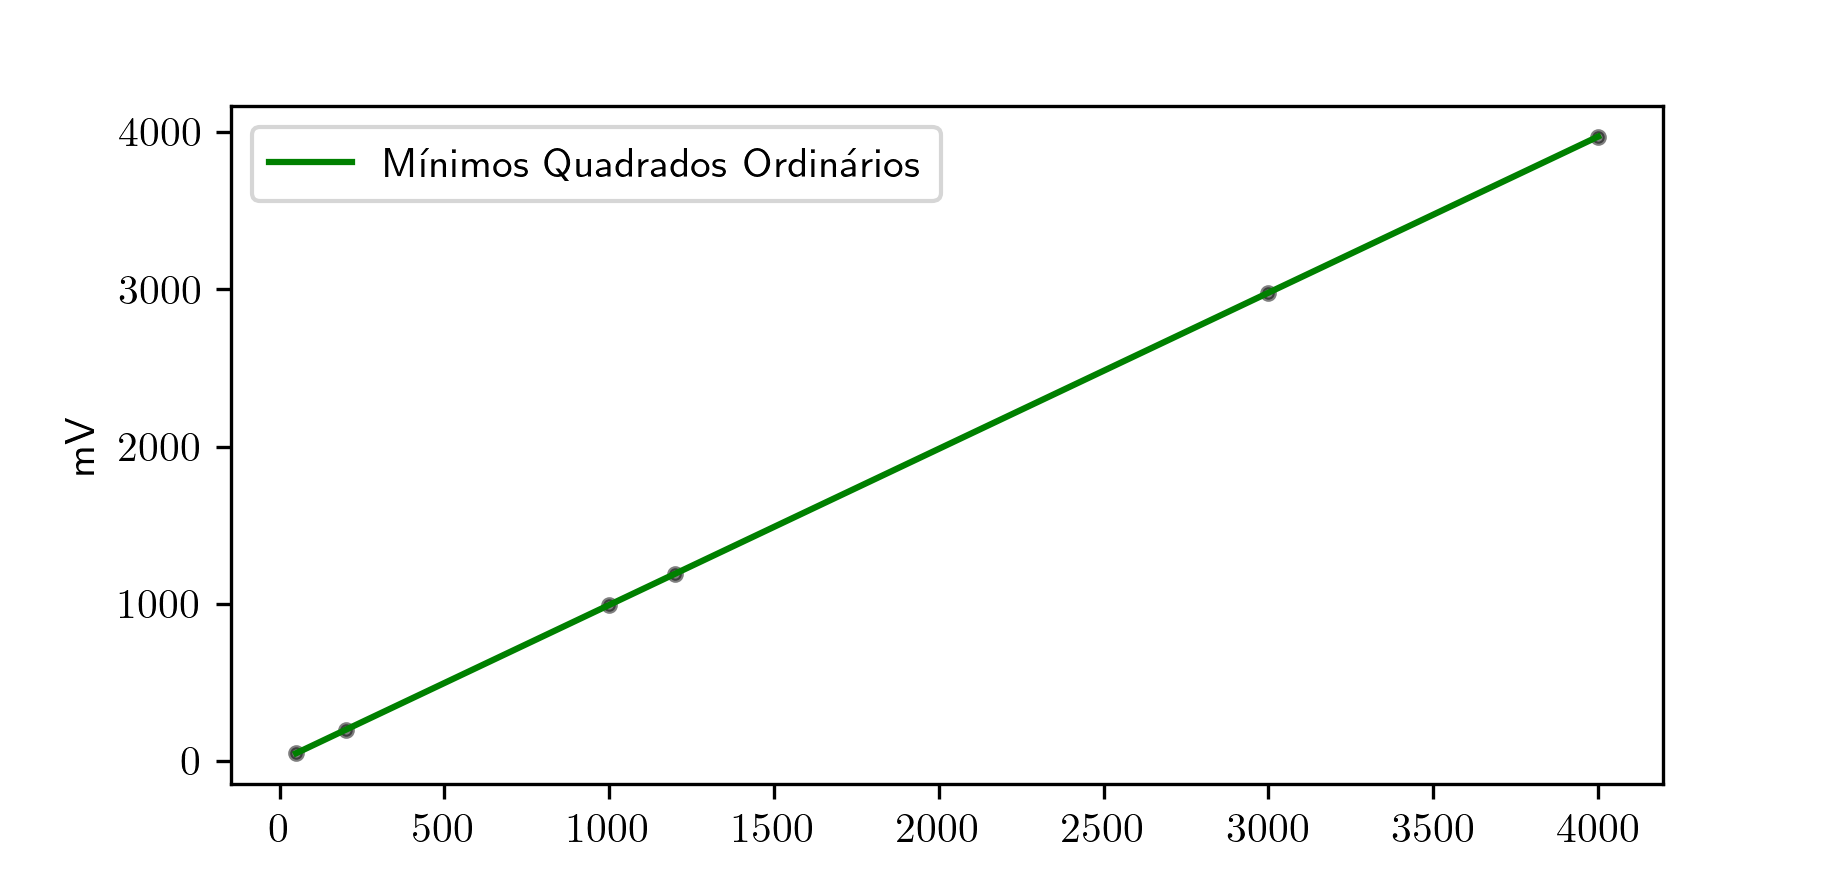
\includegraphics[width=12cm]{pictures/mqo_linha.png}
    \caption{Reta ajustada utilizando o método de Mínimos Quadrados Ordinários utilizando como sinais de entrada os valores RMS com maior erro em relação ao sinal aplicado para o canal IA}
    \label{fig:ols_line}
\end{figure}


\begin{table}[H]
\IBGEtab{%
  \caption[Sinais de corrente em 60Hz corrigidos após calibração utilizando Mínimos Quadrados Ordinários]{Sinais de corrente em 60Hz corrigidos após calibração utilizando Mínimos Quadrados Ordinários.}%
  \label{tab:tabelaerros60Aols}
} & \textbf{Valor Mín.} & \textbf{\%} & \textbf{Valor Méd.} & \textbf{\%}  \\
  \midrule
  50 & 0.6 \% & 50.0732 & 0.1464 & 49.9873 & -0.0254 & 50.6492 & 1.2984 \\
  \midrule
  200 & 0.2 \% & 199.9676 &	-0.0162 &	199.3803 &	-0.3098 & 200.2772 & 0.1386  \\
  \midrule
  1000 & 0.1 \% & 999.9097 & -0.009 & 996.6468 & -0.3353 & 1001.046 & 0.1046\\
  \midrule
  1200 & 0.1 \% & 1200.1783 & 0.0149 & 1196.2456 &	-0.3129 & 1201.7803 &	0.1484 \\
  \midrule
  3000 & 0.1 \% & 2999.8235 & -0.0059 & 2989.8713 &	-0.3376 & 2999.6535 &	-0.0116 \\
  \midrule
  4000 & 0.1 \% & 4000.1375 & 0.0034 & 3986.8394 &	-0.3290 & 4001.2924 &	0.0323 \\
  \bottomrule
\end{tabular}%
}{%
  \fonte{Produzido pelo autor.}%
 % \nota{rd representa o valor lido (em V).}
  %\nota{Esta é uma nota, que diz que os dados são baseados na
 % regressão linear. -- \showfont}%
  %\nota[Anotações]{Uma anotação adicional, que pode ser seguida de várias
  %outras. -- \showfont}%
  }
\end{table}


\begin{table}[H]
\IBGEtab{%
  \caption[Sinais de tensão em 60Hz corrigidos após calibração utilizando Mínimos Quadrados Ordinários]{Sinais de tensão em 60Hz corrigidos após calibração utilizando Mínimos Quadrados Ordinários.}%
  \label{tab:tabelaerros60Vols}
} & \textbf{Valor Mín.} & \textbf{\%} & \textbf{Valor Méd.} & \textbf{\%} \\
  \midrule
  9.2 & 0.1 \% & 9.3749 & 1.9014 & 9.4092 & 2.274 & 9.3173 & 1.8123\\
  \midrule
  57 & 0.1 \% & 57.7436 & 1.3046 & 57.6445 & 1.1307 & 57.7222 & 1.267   \\
  \midrule
  92 & 0.1 \% & 92.2785 & 0.3028 & 92.3173 & 0.3449 & 92.3547 & 0.3855 \\
  \midrule
  115 & 0.1 \% & 115.3321 & 0.2888 & 115.3641 & 0.3166 & 115.4533 & 0.3942 \\
  \midrule
  138 & 0.1 \% & 138.3352 &	0.2429 & 138.2648 &	0.1919 & 138.3077 &	0.2230 \\
  \midrule
  161 & 0.1 \% & 161.3615 & 0.2245 & 161.3868 &	0.2402 & 161.3902 &	0.2423\\
  \bottomrule
\end{tabular}%
}{%
  \fonte{Produzido pelo autor.}%
 % \nota{rd representa o valor lido (em V).}
  %\nota{Esta é uma nota, que diz que os dados são baseados na
 % regressão linear. -- \showfont}%
  %\nota[Anotações]{Uma anotação adicional, que pode ser seguida de várias
  %outras. -- \showfont}%
  }
\end{table}

Como é possível observar na tabela \ref{tab:tabelaerros60Aols}, houve significativa melhora nos erros relativos aos sinais de corrente. Após a calibração utilizando os pontos de erro máximo, os valores lidos em toda a faixa de aquisição passaram a se encontrar dentro da tolerância do equipamento. Entretanto, é perceptível que a calibração utilizando os pontos de erro mínimo e erro médio acabou por gerar coeficientes que, na maioria dos pontos, não reduziram tanto os erros quanto a calibração feita utilizando os pontos de erro máximo. Apesar disto, mesmo nestes casos as leituras ficaram dentro das especificações.

Já para os dados de tensão expostos na tabela \ref{tab:tabelaerros60Vols}, apesar da diminuição nos erros em toda a faixa de aquisição, estes ainda não se encontram dentro do especificado pelo fabricante (0.1 \% de 0.08Vn até 2Vn) em nenhum dos conjuntos de dados usados para calibração.

Com sinais aplicados com 50Hz, obtém-se os valores expostos nas tabelas \ref{tab:tabelaerros50Aols} e \ref{tab:tabelaerros50Vols} após a correção utilizando os coeficientes de primeira ordem utilizando o método de mínimos quadrados ordinários.

\begin{table}[H]
\IBGEtab{%
  \caption[Sinais de corrente em 50Hz corrigidos após calibração utilizando Mínimos Quadrados Ordinários]{Sinais de corrente em 50Hz corrigidos após calibração utilizando Mínimos Quadrados Ordinários.}%
  \label{tab:tabelaerros50Aols}
} & \textbf{Valor Mín.} & \textbf{\%} & \textbf{Valor Méd.} & \textbf{\%}  \\
  \midrule
  50 & 0.6 \% & 50.3303 & 0.6606 & 50.4465 & 0.893 & 49.6527 & -0.6947 \\
  \midrule
  200 & 0.2 \% & 199.8804 & -0.0598 & 200.5212 & 0.2606 & 199.4184 & -0.2908  \\
  \midrule
  1000 & 0.1 \% & 999.6978 & -0.0302 & 1001.8729 & 0.1873 & 1000.1444 & 0.0144\\
  \midrule
  1200 & 0.1 \% & 1200.0672 & 0.0056 & 1199.4922 & -0.0423 & 1197.7319 & -0.189 \\
  \midrule
  3000 & 0.1 \% & 2999.7407 & -0.0086 & 3002.3547 & 0.0785 & 2994.7691 & -0.1744 \\
  \midrule
  4000 & 0.1 \% & 4000.231 & 0.0058 & 4006.1437 & 0.1536 & 4002.1524 & 0.0538 \\
  \bottomrule
\end{tabular}%
}{%
  \fonte{Produzido pelo autor.}%
 % \nota{rd representa o valor lido (em V).}
  %\nota{Esta é uma nota, que diz que os dados são baseados na
 % regressão linear. -- \showfont}%
  %\nota[Anotações]{Uma anotação adicional, que pode ser seguida de várias
  %outras. -- \showfont}%
  }
\end{table}

\begin{table}[H]
\IBGEtab{%
  \caption[Sinais de tensão em 50Hz corrigidos após calibração utilizando Mínimos Quadrados Ordinários]{Sinais de tensão em 50Hz corrigidos após calibração utilizando Mínimos Quadrados Ordinários.}%
  \label{tab:tabelaerros50Vols}
} & \textbf{Valor Mín.} & \textbf{\%} & \textbf{Valor Méd.} & \textbf{\%} \\
  \midrule
  9.2 & 0.1 \% & 9.5037 & 3.3011 & 10.2354 & 11.2543 & 9.3615 & 1.7554\\
  \midrule
  57 & 0.1 \% & 57.7989 & 1.4015 & 61.4752 & 7.8512 & 57.6901 & 1.2107\\
  \midrule
  92 & 0.1 \% & 92.3592 & 0.3904 & 109.4042 & 18.9176 & 92.3574 & 0.3885\\
  \midrule
  115 & 0.1 \% & 115.3925 & 0.3413 & 135.9996 & 18.2605 & 115.1646 & 0.1431 \\
  \midrule
  138 & 0.1 \% & 138.4393 & 0.3184 & 140.8817 & 2.0882 & 138.1461 & 0.1059 \\
  \midrule
  161 & 0.1 \% & 161.4813 & 0.299 & 163.7498 & 1.7079 & 161.4896 & 0.3041\\
  \bottomrule
\end{tabular}%
}{%
  \fonte{Produzido pelo autor.}%
 % \nota{rd representa o valor lido (em V).}
  %\nota{Esta é uma nota, que diz que os dados são baseados na
 % regressão linear. -- \showfont}%
  %\nota[Anotações]{Uma anotação adicional, que pode ser seguida de várias
  %outras. -- \showfont}%
  }
\end{table}

Analisando os resultados para sinais de corrente, é perceptível que o único ponto a estar fora das especificações do fabricante (0.6 $\%$) possui 50 mA de amplitude, tanto utilizando como valores de entrada os valores RMS dos ciclos com maior erro em relação ao valor aplicado, quanto utilizando os valores RMS com erro mínimo por ciclo ou o valor médio entre os valores RMS obtidos em todos os ciclos de aquisição.  Para sinais de corrente com amplitude maior, a calibração mostrou-se suficiente. Nos resultados para sinais de tensão, observa-se um erro máximo superando os 0.1 $\%$ máximos segundo o fabricante para toda a extensão de valores aplicados, tanto utilizando como valores de entrada os valores RMS com maior erro em relação ao valor aplicado quanto os valores com menor, bem como o erro entre o valor RMS médio entre todos os ciclos de sinal capturados. 

A tabela \ref{tab:tabelaerros60olsrsq} expõe os valores de $R^2$ para cada um dos conjuntos de dados usados para a linearização. É observável que, uma vez que a linearização traz resultados muito próximos dos nominais, este valor é muito próximo de 1. Entretanto, como critério de avaliação, o coeficiente $R^2$ traz poucas informações, pois para todos os valores de entrada este coeficiente torna-se muito próximo de 1.

\begin{table}[H]
\IBGEtab{%
  \caption[Coeficientes $R^2$ para a linearização por Mínimos Quadrados Ordinários]{Coeficientes $R^2$ para a linearização por Mínimos Quadrados Ordinários.}%
  \label{tab:tabelaerros60olsrsq}
}{%
  \begin{tabular}{ccc}
  \toprule
   \textbf{Canal IA} &  &  \\
  \midrule
 \textbf{$R^2$ Erro máximo} & \textbf{ $R^2$ Erro Mínimo} & \textbf{$R^2$ Erro médio}   \\
  \midrule
  999999992454582 & 0.999999681815048 & 0.99999977198064\\
    \toprule
   \textbf{Canal VC} &  &  \\
     \midrule
 \textbf{$R^2$ Erro máximo} & \textbf{ $R^2$ Erro Mínimo} & \textbf{$R^2$ Erro médio}   \\
    \midrule
  0.999987761633336 & 0.999992528523623 & 0.999990248990353\\
    \bottomrule
\end{tabular}%
}{%
  \fonte{Produzido pelo autor.}%
 % \nota{rd representa o valor lido (em V).}
  %\nota{Esta é uma nota, que diz que os dados são baseados na
 % regressão linear. -- \showfont}%
  %\nota[Anotações]{Uma anotação adicional, que pode ser seguida de várias
  %outras. -- \showfont}%
  }
\end{table}


\section{Mínimos Quadrados Ponderados}

Já utilizando o método dos mínimos quadrados ponderados, os resultados da calibração estão expostos nas tabelas \ref{tab:tabelaerros60Awls} para corrente e \ref{tab:tabelaerros60Vwls} para tensão. É digno de menção que o vetor de a matriz diagonal de pesos utilizada é inversamente proporcional aos erros máximos especificados pelo fabricante nas tabelas \ref{tab:specsMEA} e \ref{tab:specsMEV}, isto é: os sinais aplicados em regiões de aquisição com erro menor permitido terão peso maior na linearização. A figura \ref{fig:wls_line} ilustra a reta ajustada após a aplicação deste método.

\begin{figure}[H]
    \centering
    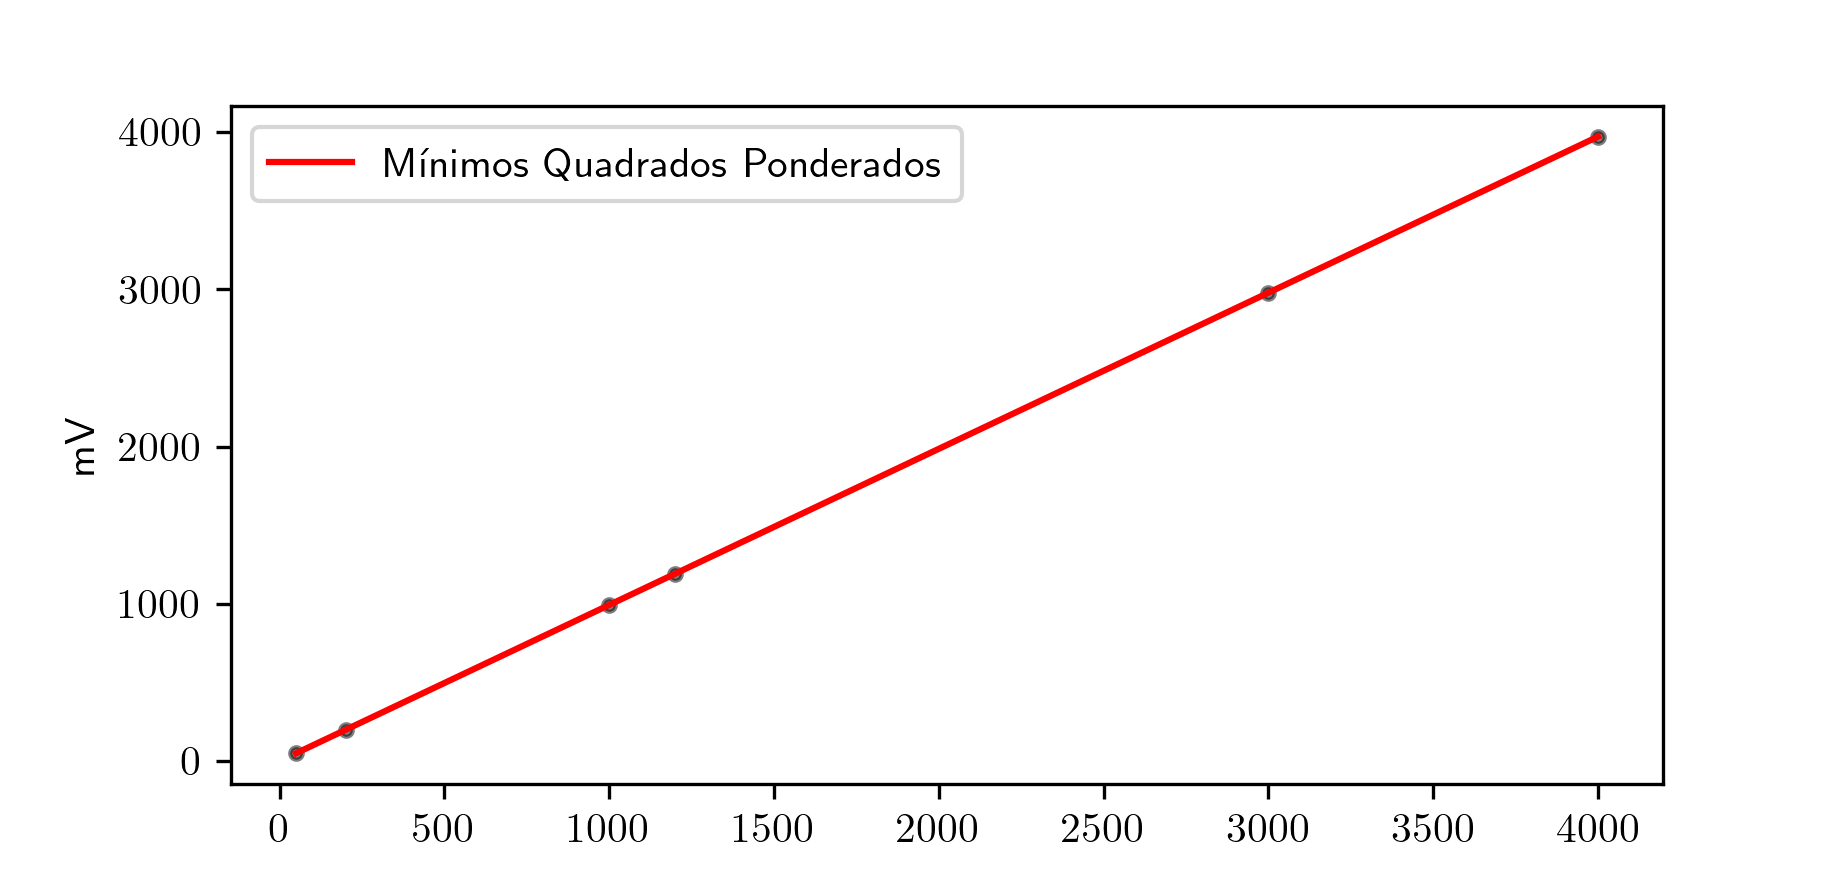
\includegraphics[width=12cm]{pictures/mqp_linha.png}
    \caption{Reta ajustada utilizando o método de Mínimos Quadrados Ponderados utilizando como sinais de entrada os valores RMS com maior erro em relação ao sinal aplicado para o canal IA}
    \label{fig:wls_line}
\end{figure}

\begin{table}[H]
\IBGEtab{%
  \caption[Sinais de corrente com frequência de 60Hz corrigidos após calibração utilizando Mínimos Quadrados Ponderados]{[Sinais de corrente com frequência de 60Hz corrigidos após calibração utilizando Mínimos Quadrados Ponderados.}%
  \label{tab:tabelaerros60Awls}
} & \textbf{Valor Mín.} & \textbf{\%} & \textbf{Valor Méd.} & \textbf{\%} \\
  \midrule
  50 & 0.6 \% & 50.0988 & 0.1976 & 50.7535 & 1.507 & 51.0945	& 2.1889\\
  \midrule
  200 & 0.2 \% & 199.9982 & -0.0009 & 200.1686 & 0.0843 & 200.7633 & 0.3816\\
  \midrule
  1000 & 0.1 \% & 999.9671 & -0.0033 & 1001.1913 & 0.1191 & 1001.7502 & 0.175\\
  \midrule
  1200 & 0.1 \% & 1200.2424 & 0.0202 & 1201.5306 & 0.1275 & 1202.5392 & 0.2116\\
  \midrule
  3000 & 0.1 \% & 2999.9478 & -0.0017 & 2999.9857 & -0.0005 & 3000.9022 & 0.0301\\
  \midrule
  4000 & 0.1 \% & 4000.2953 & 0.0074 & 4002.8304 & 0.0708 & 4002.814 & 0.0704\\
  \bottomrule
\end{tabular}%
}{%
  \fonte{Produzido pelo autor.}%
 % \nota{rd representa o valor lido (em V).}
  %\nota{Esta é uma nota, que diz que os dados são baseados na
 % regressão linear. -- \showfont}%
  %\nota[Anotações]{Uma anotação adicional, que pode ser seguida de várias
  %outras. -- \showfont}%
  }
\end{table}

\begin{table}[H]
\IBGEtab{%
  \caption[Sinais de tensão com frequência de 60Hz corrigidos após calibração utilizando Mínimos Quadrados Ponderados]{Sinais de tensão com frequência de 60Hz corrigidos após calibração utilizando Mínimos Quadrados Ponderados.}%
  \label{tab:tabelaerros60Vwls}
} & \textbf{Valor Mín.} & \textbf{\%} & \textbf{Valor Méd.} & \textbf{\%} \\
  \midrule
  9.2 & 0.1 \% &  9.3749 & 1.9014 & 9.4092 & 2.274 & 9.4173 & 2.3623\\
  \midrule
  57 & 0.1 \% & 57.7436 & 1.3046 & 57.6445 & 1.1307 & 57.7222 & 1.267\\
  \midrule
  92 & 0.1 \% & 92.2785 & 0.3028 & 92.3173 & 0.3449 & 92.3547 & 0.3855\\
  \midrule
  115 & 0.1 \% & 115.3321 & 0.2888 & 115.3641 & 0.3166 & 115.4533 & 0.3942 \\
  \midrule
  138 & 0.1 \% & 138.3352 & 0.2429 & 138.2648 & 0.1919 & 138.3077 & 0.223\\
  \midrule
  161 & 0.1 \% & 161.3615 & 0.2245 & 161.3868 & 0.2402 & 161.3902 & 0.2423\\
  \bottomrule
\end{tabular}%
}{%
  \fonte{Produzido pelo autor.}%
 % \nota{rd representa o valor lido (em V).}
  %\nota{Esta é uma nota, que diz que os dados são baseados na
 % regressão linear. -- \showfont}%
  %\nota[Anotações]{Uma anotação adicional, que pode ser seguida de várias
  %outras. -- \showfont}%
  }
\end{table}

Da mesma forma que no método anterior, é possível verificar que a calibração do canal de tensão mostrou-se insuficiente para trazer a leitura dos sinais de tensão para dentro das especificações do equipamento, tendo como piores casos os sinais com amplitude menor. Para o canal de corrente, são observados resultados semelhantes utilizando os pontos com erro máximo como entrada do algoritmo. Entretanto, utilizando os pontos de erro mínimo e de erro médio, a linearização acabou piorando o erro nos pontos com menor amplitude de corrente, sendo suficiente para não atender as especificações.

Utilizando os sinais de 50Hz como entrada do método, obtém-se as tabelas \ref{tab:tabelaerros50Awls} \ref{tab:tabelaerros50Vwls} após aplicação dos coeficientes gerados para correção.

Com  este método, foram obtidos resultados dentro dos máximos permitidos pelo fabricante para toda a faixa de aquisição de corrente utilizando como valores de entrada os valores RMS com erro máximo entre os ciclos e erro médio entre todos os ciclos RMS. Utilizando o erro mínimo por ciclo como entrada para o método, o sinal de 50mA permanece fora das especificações do fabricante.

Para as aquisições de tensão, em nenhum dos grupos de sinais de entrada foi possível atingir os mínimos descritos na documentação do equipamento (0.1 \%).

\begin{table}[H]
\IBGEtab{%
  \caption[Sinais de corrente com frequência de 50Hz corrigidos após calibração utilizando Mínimos Quadrados Ponderados]{Sinais de corrente com frequência de 50Hz corrigidos após calibração utilizando Mínimos Quadrados Ponderados.}%
  \label{tab:tabelaerros50Awls}
} & \textbf{Valor Mín.} & \textbf{\%} & \textbf{Valor Méd.} & \textbf{\%} \\
  \midrule
  50 & 0.6 \% & 50.2551 & 0.5102 & 57.6585 & 15.3169 & 50.2479 & 0.4957\\
  \midrule
  200 & 0.2 \% & 199.8071 & -0.0965 & 199.6745 & -0.1627 & 200.0427 & 0.0213\\
  \midrule
  1000 & 0.1 \% & 999.6346 & -0.0365 & 999.3963 & -0.0604 & 1001.5594 & 0.1559\\
  \midrule
  1200 & 0.1 \% & 1200.0065 & 0.0005 & 1196.9341 & -0.2555 & 1199.3174 & -0.0569\\
  \midrule
  3000 & 0.1 \% & 2999.7027 & -0.0099 & 2999.0531 & -0.0316 & 2997.9047 & -0.0698\\
  \midrule
  4000 & 0.1 \% & 4000.2057 & 0.0051 & 4002.4282 & 0.0607 & 4006.1568 & 0.1539\\
  \bottomrule
\end{tabular}%
}{%
  \fonte{Produzido pelo autor.}%
 % \nota{rd representa o valor lido (em V).}
  %\nota{Esta é uma nota, que diz que os dados são baseados na
 % regressão linear. -- \showfont}%
  %\nota[Anotações]{Uma anotação adicional, que pode ser seguida de várias
  %outras. -- \showfont}%
  }
\end{table}

\begin{table}[H]
\IBGEtab{%
  \caption[Sinais de tensão com frequência de 50Hz corrigidos após calibração utilizando Mínimos Quadrados Ponderados]{Sinais de tensão com frequência de 50Hz corrigidos após calibração utilizando Mínimos Quadrados Ponderados.}%
  \label{tab:tabelaerros50Vwls}
} & \textbf{Valor Mín.} & \textbf{\%} & \textbf{Valor Méd.} & \textbf{\%} \\
  \midrule
  9.2 & 0.1 \% & 9.3749 & 1.9014 & 9.4092 & 2.274 & 9.4173 & 2.3623\\
  \midrule
  57 & 0.1 \% & 57.7436 & 1.3046 & 57.6445 & 1.1307 & 57.7222 & 1.267\\
  \midrule
  92 & 0.1 \% & 92.2785 & 0.3028 & 92.3173 & 0.3449 & 92.3547 & 0.3855\\
  \midrule
  115 & 0.1 \% & 115.3321 & 0.2888 & 115.3641 & 0.3166 & 115.4533 & 0.3942 \\
  \midrule
  138 &  0.1 \% & 138.3352 & 0.2429 & 138.2648 & 0.1919 & 138.3077 & 0.223\\
  \midrule
  161 & 0.1 \% & 161.3615 & 0.2245 & 161.3868 & 0.2402 & 161.3902 & 0.2423\\
  \bottomrule
\end{tabular}%
}{%
  \fonte{Produzido pelo autor.}%
 % \nota{rd representa o valor lido (em V).}
  %\nota{Esta é uma nota, que diz que os dados são baseados na
 % regressão linear. -- \showfont}%
  %\nota[Anotações]{Uma anotação adicional, que pode ser seguida de várias
  %outras. -- \showfont}%
  }
\end{table}

Da mesma forma que no método de mínimos quadrados ordinários, os coeficientes de determinação  $R^2$ não trazem informações muito úteis na análise, exceto por descrever a boa linearização obtida pelo algoritmo. A tabela \ref{tab:tabelaerros60wlsrsq} expõe estes valores.

\begin{table}[H]
\IBGEtab{%
  \caption[Coeficientes $R^2$ para a linearização por Mínimos Quadrados Ponderados]{Coeficientes $R^2$ para a linearização por Mínimos Quadrados Ponderados.}%
  \label{tab:tabelaerros60wlsrsq}
}{%
  \begin{tabular}{ccc}
  \toprule
   \textbf{Canal IA} &  &  \\
  \midrule
 \textbf{$R^2$ Erro máximo} & \textbf{ $R^2$ Erro Mínimo} & \textbf{$R^2$ Erro médio}   \\
  \midrule
 0.999999900283003 & 0.99999952000389 & 0.99999960002109\\
    \toprule
   \textbf{Canal VC} &  &  \\
     \midrule
 \textbf{$R^2$ Erro máximo} & \textbf{ $R^2$ Erro Mínimo} & \textbf{$R^2$ Erro médio}   \\
    \midrule
0.9999835900083 & 0.99999036982379 & 0.999987420008623\\
    \bottomrule
\end{tabular}%
}{%
  \fonte{Produzido pelo autor.}%
 % \nota{rd representa o valor lido (em V).}
  %\nota{Esta é uma nota, que diz que os dados são baseados na
 % regressão linear. -- \showfont}%
  %\nota[Anotações]{Uma anotação adicional, que pode ser seguida de várias
  %outras. -- \showfont}%
  }
\end{table}

\section{Mínimos Desvios Absolutos}

Corrigindo os valores expostos nas tabelas \ref{tab:specsMEA} e \ref{tab:specsMEV} com os coeficientes de primeira ordem resultantes da aplicação do método de mínimos desvios absolutos, são obtidos os resultados expostos nas tabelas \ref{tab:tabelaerros60Alad} e \ref{tab:tabelaerros60Vlad}. A figura \ref{fig:lad_line} ilustra a reta ajustada após a aplicação deste método.

\begin{figure}[H]
    \centering
    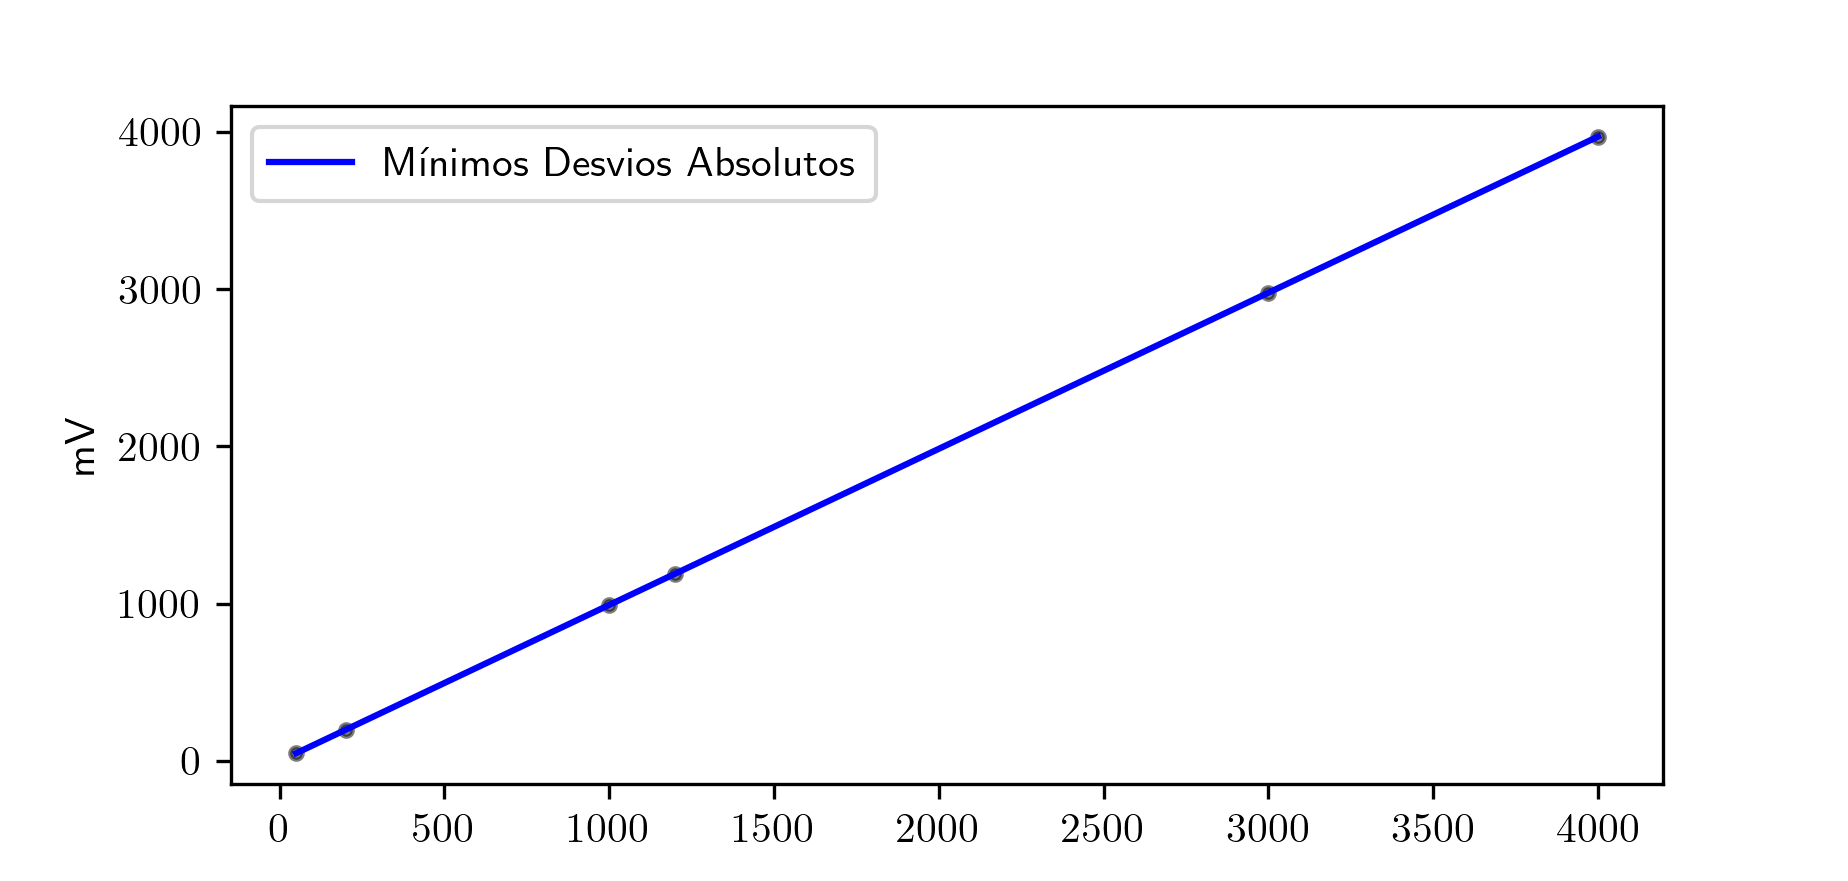
\includegraphics[width=12cm]{pictures/mda_linha.png}
    \caption{Reta ajustada utilizando o método de Mínimos Desvios Absolutos utilizando como sinais de entrada os valores RMS com maior erro em relação ao sinal aplicado para o canal IA}
    \label{fig:lad_line}
\end{figure}

\begin{table}[H]
\IBGEtab{%
  \caption[Sinais de corrente com 60Hz corrigidos após calibração utilizando Mínimos Desvios Absolutos]{Sinais de corrente corrigidos após calibração utilizando Mínimos Desvios Absolutos.}%
  \label{tab:tabelaerros60Alad}
} & \textbf{Valor Mín.} & \textbf{\%} & \textbf{Valor Méd.} & \textbf{\%} \\
  \midrule
  50 & 0.6 \% & 50.015 & 0.0299 & 50.4466 & 0.8932 & 50.8247 & 1.6494\\
  \midrule
  200 & 0.2 \% & 199.9026 & -0.0487 & 199.7801 & -0.1099 & 200.4405 & 0.2202\\
  \midrule
  1000 & 0.1 \% & 999.809 & -0.0191 & 1000.3653 & 0.0365 & 1001.1435 & 0.1143\\
  \midrule
  1200 & 0.1 \% & 1200.0687 &  0.0057 & 1200.5952 & 0.0496 & 1201.8613 & 0.1551\\
  \midrule
  3000 & 0.1 \% & 2999.6333 & -0.0122 & 2998.0683 & -0.0644 & 2999.5868 & -0.0138 \\
  \midrule
  4000 & 0.1 \% & 3999.9026 & -0.0024 & 4000.3653 & 0.0091 & 4001.1435 & 0.0286\\
  \bottomrule
\end{tabular}%
}{%
  \fonte{Produzido pelo autor.}%
 % \nota{rd representa o valor lido (em V).}
  %\nota{Esta é uma nota, que diz que os dados são baseados na
 % regressão linear. -- \showfont}%
  %\nota[Anotações]{Uma anotação adicional, que pode ser seguida de várias
  %outras. -- \showfont}%
  }
\end{table}

\begin{table}[H]
\IBGEtab{%
  \caption[Sinais de tensão com 60Hz corrigidos após calibração utilizando Mínimos Desvios Absolutos]{Sinais de tensão corrigidos após calibração utilizando Mínimos Desvios Absolutos.}%
  \label{tab:tabelaerros60Vlad}
} & \textbf{Valor Mín.} & \textbf{\%} & \textbf{Valor Méd.} & \textbf{\%} \\
  \midrule
  9.2 & 0.1 \% & 9.3201 &	1.3055 &	9.939 &	8.0331 & 10.0301 & 9.0226\\
  \midrule
  57 & 0.1 \% & 57.6822 & 1.1969 & 58.3836 & 2.4274 & 58.5599 & 2.7367\\
  \midrule
  92 & 0.1 \% & 92.2125 & 0.2309 & 93.2068 & 1.3118 & 93.3537 & 1.4714\\
  \midrule
  115 & 0.1 \% & 115.2629 & 0.2286 & 116.3537 & 1.1771 & 116.5599 & 1.3564\\
  \midrule
  138 & 0.1 \% & 138.2629 & 0.1905 & 139.3537 & 0.9809 & 139.5208 & 1.102\\
  \midrule
  161 & 0.1 \% & 161.2861 & 0.1777 & 162.576 & 0.9789 & 162.7107 & 1.0625\\
  \bottomrule
\end{tabular}%
}{%
  \fonte{Produzido pelo autor.}%
 % \nota{rd representa o valor lido (em V).}
  %\nota{Esta é uma nota, que diz que os dados são baseados na
 % regressão linear. -- \showfont}%
  %\nota[Anotações]{Uma anotação adicional, que pode ser seguida de várias
  %outras. -- \showfont}%
  }
\end{table}

Utilizando o método dos Mínimos Desvios Absolutos com sinais com frequência de 60 Hz, a linearização à partir dos pontos de maior erro em relação à amplitude dos sinais de corrente aplicados trouxe resultados melhores que nos dois métodos anteriores para os pontos máximo e mínimo. Para valores mais próximos do nominal, este método teve resultados semelhantes aos dois métodos anteriores. Da mesma forma que os dois métodos anteriores, a calibração utilizando os pontos de erro mínimo e erro médio trouxeram resultados insuficientes para fazer com que o erro fique dentro das suas próprias especificações.

Com sinais de entrada com frequência de 50 Hz, os resultados estão expostos nas tabelas \ref{tab:tabelaerros50Alad} e \ref{tab:tabelaerros50Vlad}.

\begin{table}[H]
\IBGEtab{%
  \caption[Sinais de corrente com 50Hz corrigidos após calibração utilizando Mínimos Desvios Absolutos]{Sinais de corrente corrigidos após calibração utilizando Mínimos Desvios Absolutos.}%
  \label{tab:tabelaerros50Alad}
} & \textbf{Valor Mín.} & \textbf{\%} & \textbf{Valor Méd.} & \textbf{\%} \\
  \midrule
  50 & 0.6 \% & 50.2083 & 0.4167 & 57.7874 & 15.5748 & 49.8114 & -0.3772\\
  \midrule
  200 & 0.2 \% & 199.7446 & -0.1277 & 199.8041 & -0.098 & 199.3656 & -0.3172\\
  \midrule
  1000 & 0.1 \% & 999.4883 & -0.0512 & 999.5293 & -0.0471 & 999.5949 & -0.0405\\
  \midrule
  1200 & 0.1 \% & 1199.8391 & -0.0134 & 1197.068 & -0.2443 & 1197.0352 & -0.2471\\
  \midrule
  3000 & 0.1 \% & 2999.3466 & -0.0218 & 2999.1949 & -0.0268 & 2992.7333 & -0.2422 \\
  \midrule
  4000 & 0.1 \% & 3999.7447 & -0.0064 & 4002.5744 & 0.0644 & 3999.3659 & -0.0159\\
  \bottomrule
\end{tabular}%
}{%
  \fonte{Produzido pelo autor.}%
 % \nota{rd representa o valor lido (em V).}
  %\nota{Esta é uma nota, que diz que os dados são baseados na
 % regressão linear. -- \showfont}%
  %\nota[Anotações]{Uma anotação adicional, que pode ser seguida de várias
  %outras. -- \showfont}%
  }
\end{table}

\begin{table}[H]
\IBGEtab{%
  \caption[Sinais de tensão com 50Hz corrigidos após calibração utilizando Mínimos Desvios Absolutos]{Sinais de tensão corrigidos após calibração utilizando Mínimos Desvios Absolutos.}%
  \label{tab:tabelaerros50Vlad}
} & \textbf{Valor Mín.} & \textbf{\%} & \textbf{Valor Méd.} & \textbf{\%} \\
  \midrule
  9.2 & 0.1 \% & 9.2509 & 0.5532 & 11.7113 & 27.2963 & 9.8202 & 6.7416\\
  \midrule
  57 & 0.1 \% & 57.4621 & 0.8107 & 59.1408 & 3.7559 & 58.3718 & 2.4067\\
  \midrule
  92 & 0.1 \% & 91.9623 & -0.0409 & 107.8784 & 17.2592 & 93.1991 & 1.3034\\
  \midrule
  115 & 0.1 \% & 114.9556 & -0.0386 & 134.9226 & 17.324 & 116.1116 & 0.9666\\
  \midrule
  138 & 0.1 \% & 137.9624 & -0.0273 & 139.887 & 1.3674 & 139.1992 & 0.869\\
  \midrule
  161 & 0.1 \% & 160.9643 & -0.0222 & 163.1409 & 1.3297 & 162.6504 & 1.0251\\
  \bottomrule
\end{tabular}%
}{%
  \fonte{Produzido pelo autor.}%
 % \nota{rd representa o valor lido (em V).}
  %\nota{Esta é uma nota, que diz que os dados são baseados na
 % regressão linear. -- \showfont}%
  %\nota[Anotações]{Uma anotação adicional, que pode ser seguida de várias
  %outras. -- \showfont}%
  }
\end{table}

No caso da calibração do canal de tensão, nem mesmo para os pontos de erro máximo são obtidos resultados satisfatórios. A não-linearidade dos pontos é tão grande nesse canal que nem mesmo para os sinais com maior amplitude o erro é baixo o suficiente para atingir as especificações do fabricante.

\section{Análise dos Resultados}

Com o intuito de avaliar os resultados dos três métodos de maneira simultânea, o gráfico da \figref{fig:res_curr} expõe a porcentagem do erro máximo trazido pelo fabricante que os sinais de corrente possuem após as calibrações utilizando sinais de 60Hz. 

\begin{figure}[H]
    \caption{Porcentagem do erro máximo atingido para os sinais de corrente com maior erro por ciclo após a aplicação do Método dos Mínimos Quadrados Ordinários (MQO), do Método dos Mínimos Quadrados Ponderados (MQP) e do método dos Mínimos Desvios Absolutos (MDA) em 60 Hz}
    \label{fig:res_curr}
    \centering
    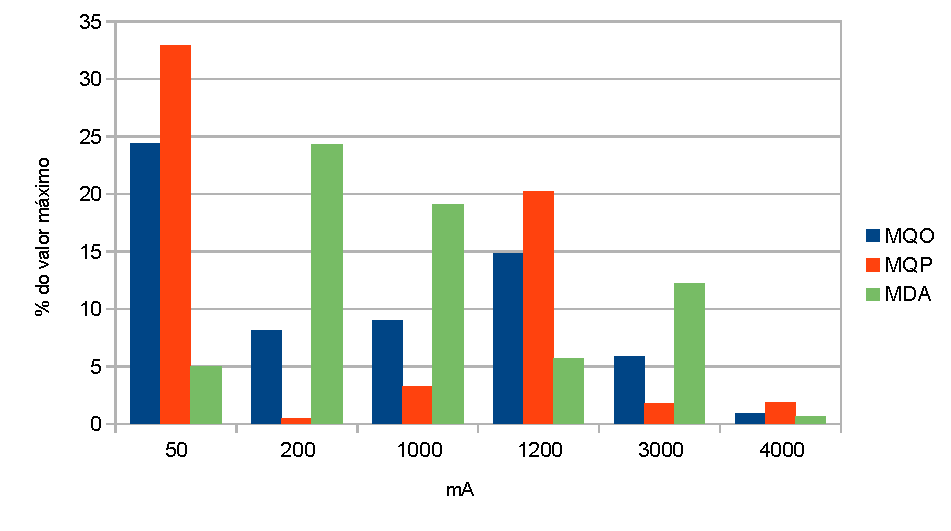
\includegraphics[width=0.9\linewidth]{pictures/max_err_IA_aftercalib60Hz}
    \fonte{o autor.}
\end{figure}

Com isto, é possível observar que o Método dos Mínimos Desvios Absolutos foi capaz de minimizar o erro mais do que os outros métodos para o sinal de menor amplitude. No entanto, para a maioria dos pontos seguintes, este método trouxe erros superiores aos outros, apesar de continuar mantendo-se dentro das especificações do fabricante. Já no Método dos Mínimos Quadrados Ordinários, os coeficientes obtidos geraram um maior erro para o ponto de menor amplitude, mas para os outros pontos este erro foi sempre menor que 15 \% do permitido. Por fim, o Método dos Mínimos Quadrados ponderados trouxe o pior erro para o sinal com amplitude mais baixa, mas exceto pelo ponto de 1.2A no qual o erro ultrapassou os 20\% do valor máximo fornecido pelo fabricante, o erro manteve-se menor que todos os outros métodos. De forma a resumir essa relação, a tabela \ref{tab:med_rescurr} expõe a média dos erros para o canal de aquisição de corrente analisado.

\begin{table}[H]
\IBGEtab{%
  \caption[Média dos erros em relação ao máximo permitido pelo fabricante para o canal de corrente IA em 60 Hz.]{Média dos erros em relação ao máximo permitido pelo fabricante para o canal de corrente IA em 60 Hz.}%
  \label{tab:med_rescurr}
}{%
  \begin{tabular}{ccc}
  \toprule
   \textbf{Canal IA} &  &   \\
  \midrule
  \textbf{Erro Médio MQO (\%)} & \textbf{Erro Médio MQP (\%)} & \textbf{Erro Médio MDA (\%)}  \\ 
  \midrule
  10.5228 &	10.0768 & 11.1635 \\
  \bottomrule
\end{tabular}%
}{%
  \fonte{Produzido pelo autor.}%
 % \nota{rd representa o valor lido (em V).}
  %\nota{Esta é uma nota, que diz que os dados são baseados na
 % regressão linear. -- \showfont}%
  %\nota[Anotações]{Uma anotação adicional, que pode ser seguida de várias
  %outras. -- \showfont}%
  }
\end{table}

Fazendo a mesma análise utilizando o canal de tensão VC, observa-se que em nenhum dos métodos os resultado foi suficiente para que as leituras possuam erros menores do que os erros máximos fornecidos pelo fabricante. A \figref{fig:res_volt} ilustra esse resultado. 

\begin{figure}[H]
    \caption{Porcentagem do erro máximo atingido para os sinais de tensão com maior erro por ciclo após a aplicação do Método dos Mínimos Quadrados Ordinários (MQO), do Método dos Mínimos Quadrados Ponderados (MQP) e do método dos Mínimos Desvios Absolutos (MDA).}
    \label{fig:res_volt}
    \centering
    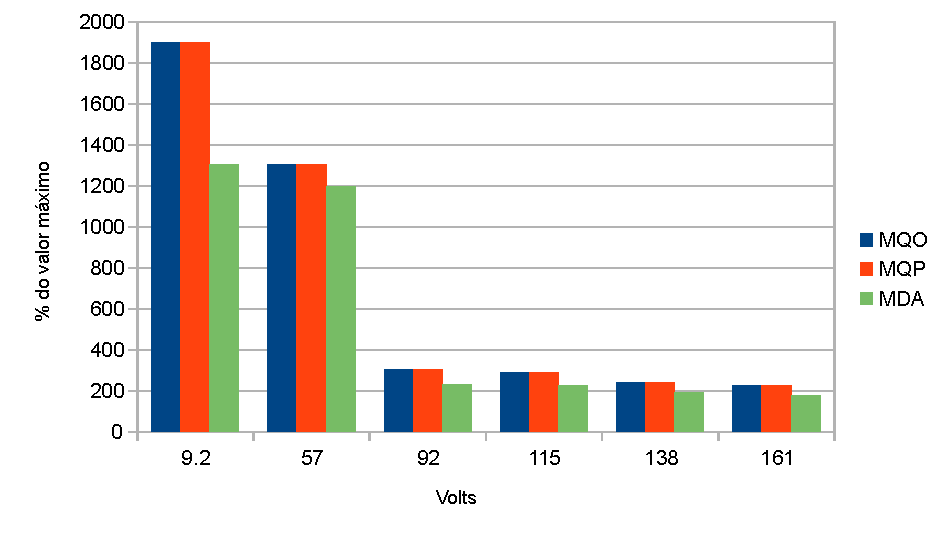
\includegraphics[width=0.9\linewidth]{pictures/max_err_VC_aftercalib60.pdf}
    \fonte{o autor.}
\end{figure}

A tabela \ref{tab:med_resvolt} expõe as médias dos erros obtidos nas três calibrações, em porcentagem do máximo permitido pelo fabricante.

\begin{table}[H]
\IBGEtab{%
  \caption[Média dos erros em relação ao máximo permitido pelo fabricante para o canal de tensão VC em 60 Hz.]{Média dos erros em relação ao máximo permitido pelo fabricante para o canal de tensão VC em 60 Hz.}%
  \label{tab:med_resvolt}
}{%
  \begin{tabular}{ccc}
  \toprule
   \textbf{Canal VC} &  &   \\
  \midrule
  \textbf{Erro Médio MQO (\%)} & \textbf{Erro Médio MQP (\%)} & \textbf{Erro Médio MDA (\%)}  \\ 
  \midrule
  710.8315 & 710.8315 & 555.013 \\
  \bottomrule
\end{tabular}%
}{%
  \fonte{Produzido pelo autor.}%
 % \nota{rd representa o valor lido (em V).}
  %\nota{Esta é uma nota, que diz que os dados são baseados na
 % regressão linear. -- \showfont}%
  %\nota[Anotações]{Uma anotação adicional, que pode ser seguida de várias
  %outras. -- \showfont}%
  }
\end{table}

Da mesma forma, utilizando sinais de entrada de 50 Hz, temos os resultados expostos nas imagens \ref{fig:res_curr50} para corrente e \ref{fig:res_volt50} para tensão. No canal de corrente, os métodos de Mínimos Quadrados Ponderados e Mínimos Desvios Absolutos em primeira ordem são suficientes para compensar as leituras e deixar o equipamento dentro das especificações do fabricante. No método de Mínimos Quadrados Ordinários, o resultado mostra-se insuficiente para 50 mA. Já para o canal de tensão, da mesma forma que utilizando sinais de entrada com 60 Hz, nenhum dos três métodos é insuficiente para a calibração em primeira ordem. As tabelas \ref{tab:med_rescurr} e \ref{tab:med_resvolt} expõem os erros médios após estas calibrações.


\begin{figure}[H]
    \caption{Porcentagem do erro máximo atingido para os sinais de corrente com maior erro por ciclo após a aplicação do Método dos Mínimos Quadrados Ordinários (MQO), do Método dos Mínimos Quadrados Ponderados (MQP) e do método dos Mínimos Desvios Absolutos (MDA) em 50 Hz}
    \label{fig:res_curr50}
    \centering
    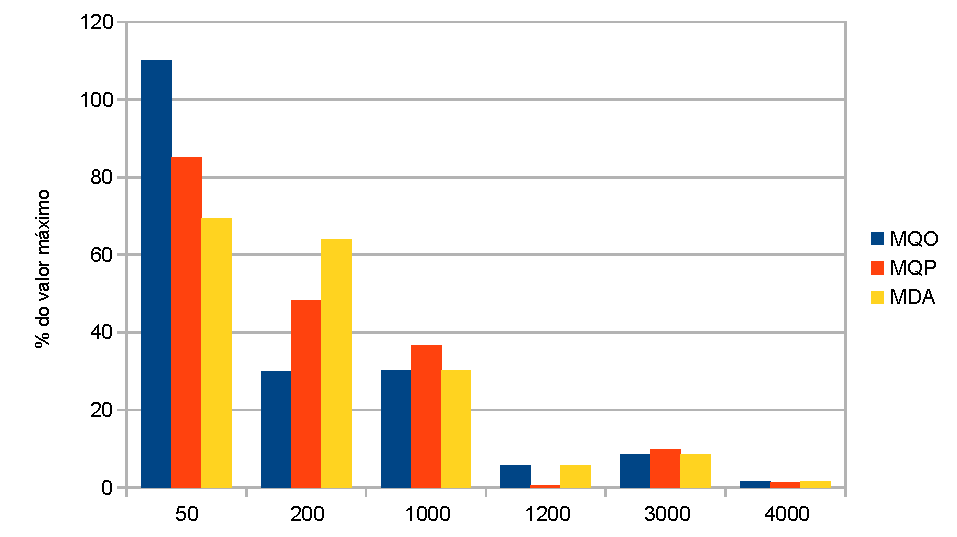
\includegraphics[width=0.9\linewidth]{pictures/max_err_IA_aftercalib50Hz.pdf}
    \fonte{o autor.}
\end{figure}

\begin{figure}[H]
    \caption{Porcentagem do erro máximo atingido para os sinais de tensão em 50 Hz com maior erro por ciclo após a aplicação do Método dos Mínimos Quadrados Ordinários (MQO), do Método dos Mínimos Quadrados Ponderados (MQP) e do método dos Mínimos Desvios Absolutos (MDA).}
    \label{fig:res_volt50}
    \centering
    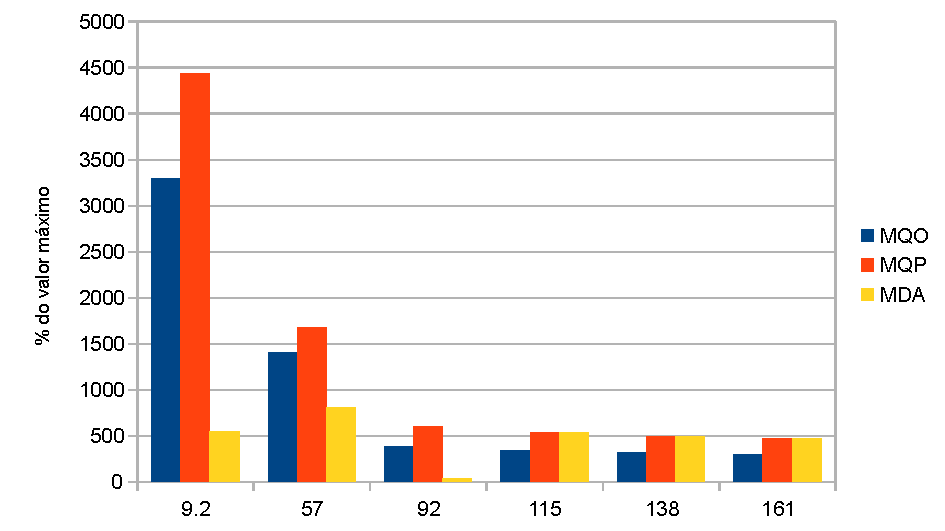
\includegraphics[width=0.9\linewidth]{pictures/max_err_VC_aftercalib50Hz.pdf}
    \fonte{o autor.}
\end{figure}

\begin{table}[H]
\IBGEtab{%
  \caption[Média dos erros em relação ao máximo permitido pelo fabricante para o canal de corrente IA em 50 Hz.]{Média dos erros em relação ao máximo permitido pelo fabricante para o canal de corrente IA em 50 Hz.}%
  \label{tab:med_rescurr50}
}{%
  \begin{tabular}{ccc}
  \toprule
   \textbf{Canal IA} &  &   \\
  \midrule
  \textbf{Erro Médio MQO (\%)} & \textbf{Erro Médio MQP (\%)} & \textbf{Erro Médio MDA (\%)}  \\ 
  \midrule
  30.9858 &	30.258 & 29.8665 \\
  \bottomrule
\end{tabular}%
}{%
  \fonte{Produzido pelo autor.}%
 % \nota{rd representa o valor lido (em V).}
  %\nota{Esta é uma nota, que diz que os dados são baseados na
 % regressão linear. -- \showfont}%
  %\nota[Anotações]{Uma anotação adicional, que pode ser seguida de várias
  %outras. -- \showfont}%
  }
\end{table}


\begin{table}[H]
\IBGEtab{%
  \caption[Médias dos erros em relação ao máximo permitido pelo fabricante para o canal de tensão VC em 50 Hz.]{Médias dos erros em relação ao máximo permitido pelo fabricante para o canal de tensão VC em 50 Hz.}%
  \label{tab:med_resvolt50}
}{%
  \begin{tabular}{ccc}
  \toprule
   \textbf{Canal VC} &  &   \\
  \midrule
  \textbf{Erro Médio MQO (\%)} & \textbf{Erro Médio MQP (\%)} & \textbf{Erro Médio MDA (\%)}  \\ 
  \midrule
  1008.6213 & 1369.9299 & 484.2613 \\
  \bottomrule
\end{tabular}%
}{%
  \fonte{Produzido pelo autor.}%
 % \nota{rd representa o valor lido (em V).}
  %\nota{Esta é uma nota, que diz que os dados são baseados na
 % regressão linear. -- \showfont}%
  %\nota[Anotações]{Uma anotação adicional, que pode ser seguida de várias
  %outras. -- \showfont}%
  }
\end{table}

Com o intuito de tentar diminuir estes erros, é proposta também uma calibração em segunda ordem para o canal de tensão. Neste caso, ao invés de tentar-se adequar os valores a uma reta, os valores são adequados a uma parábola. Diferentemente dos métodos em primeira ordem, em segunda ordem a equação que resolve a calibração é observada na equação \ref{eq:sec_order}. 

\begin{equation}\label{eq:sec_order}
y_i = \gamma x_i^2 + \beta x_i + \alpha
\end{equation}

Neste caso, há um termo a mais, $\gamma$, capaz de compensar os erros em segunda ordem obtidos ao empregar os três métodos de calibração apresentados neste trabalho.  

Os resultados desta proposta estão na \figref{fig:res_volt2nd} para os três métodos descritos no capítulo anterior.

\begin{figure}[H]
    \caption{Porcentagem do erro máximo atingido para os sinais de tensão com maior erro por ciclo em 60 Hz após a aplicação do Método dos Mínimos Quadrados Ordinários (MQO), do Método dos Mínimos Quadrados Ponderados (MQP) e do método dos Mínimos Desvios Absolutos (MDA), todos em segunda ordem.}
    \label{fig:res_volt2nd}
    \centering
    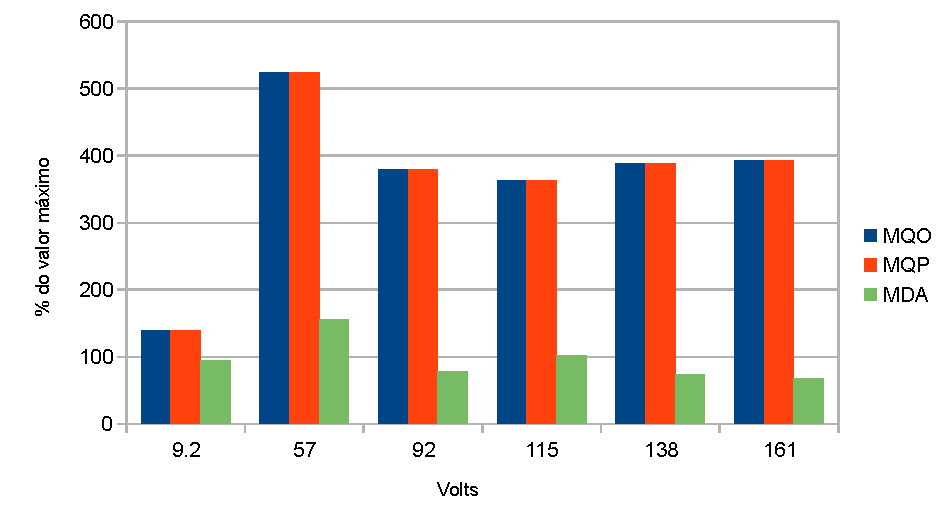
\includegraphics[width=0.9\linewidth]{pictures/max_err_VC_aftercalib60_2nd.pdf}
    \fonte{o autor.}
\end{figure}

Como já é possível perceber, há uma substancial diminuição nos erros, principalmente utilizando a calibração de Mínimos Desvios Absolutos. Apenas os pontos de 57V e 115V os mínimos fornecidos pelo fabricante, o que vale dizer que para os outros quatro pontos o erro manteve-se menor que 0.1$\%$. As médias dos erros após as linearizações em segunda ordem evidenciam ainda mais essa melhora e podem ser observadas na tabela \ref{tab:tabelaerros60Alad2nd}.

\begin{table}[H]
\IBGEtab{%
  \caption[Médias dos erros em relação ao máximo permitido pelo fabricante para o canal de tensão VC em 60 Hz após as calibrações em segunda ordem.]{Médias dos erros em relação ao máximo permitido pelo fabricante para o canal de tensão VC em 60 Hz após as calibrações em segunda ordem.}%
  \label{tab:tabelaerros60Alad2nd}
}{%
  \begin{tabular}{ccc}
  \toprule
   \textbf{Canal VC} &  &   \\
  \midrule
  \textbf{Erro Médio MQO (\%)} & \textbf{Erro Médio MQP (\%)} & \textbf{Erro Médio MDA (\%)}  \\ 
  \midrule
  359.3539 & 359.3539 &	100.9507 \\
  \bottomrule
\end{tabular}%
}{%
  \fonte{Produzido pelo autor.}%
 % \nota{rd representa o valor lido (em V).}
  %\nota{Esta é uma nota, que diz que os dados são baseados na
 % regressão linear. -- \showfont}%
  %\nota[Anotações]{Uma anotação adicional, que pode ser seguida de várias
  %outras. -- \showfont}%
  }
\end{table}
  
    Procedendo da mesma forma para a calibração em segunda ordem do canal VC com sinais de 50 Hz, são obtidos os resultados expostos na \figref{fig:res_volt2nd50}. Similarmente aos resultados obtidos em 60 Hz, a calibração utilizando o Método de Desvios Absolutos trouxe os melhores resultados observando o erro médio entre todos os pontos, mas ainda assim, este método se mostrou insuficiente para adequar o canal de aquisição com as especificações fornecidas pelo fabricante. A tabela \ref{tab:tabelaerros50Alad2nd} expõe estes resultados.

  \begin{figure}[H]
    \caption{Porcentagem do erro máximo atingido para os sinais de tensão com maior erro por ciclo em 50 Hz após a aplicação do Método dos Mínimos Quadrados Ordinários (MQO), do Método dos Mínimos Quadrados Ponderados (MQP) e do método dos Mínimos Desvios Absolutos (MDA), todos em segunda ordem.}
    \label{fig:res_volt2nd50}
    \centering
    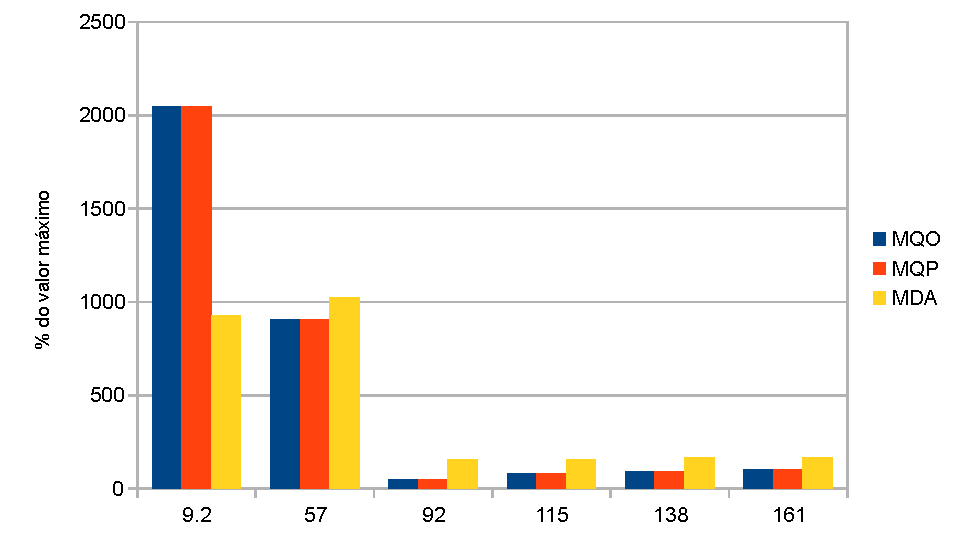
\includegraphics[width=0.9\linewidth]{pictures/max_err_VC_aftercalib50_2nd.pdf}
    \fonte{o autor.}
\end{figure}

\begin{table}[H]
\IBGEtab{%
  \caption[Médias dos erros em relação ao máximo permitido pelo fabricante para o canal de tensão VC em 50 Hz após as calibrações em segunda ordem.]{Médias dos erros em relação ao máximo permitido pelo fabricante para o canal de tensão VC em 50 Hz após as calibrações em segunda ordem.}%
  \label{tab:tabelaerros50Alad2nd}
}{%
  \begin{tabular}{ccc}
  \toprule
   \textbf{Canal VC} &  &   \\
  \midrule
  \textbf{Erro Médio MQO (\%)} & \textbf{Erro Médio MQP (\%)} & \textbf{Erro Médio MDA (\%)}  \\ 
  \midrule
  544.9508 & 544.9508 &	433.0842 \\
  \bottomrule
\end{tabular}%
}{%
  \fonte{Produzido pelo autor.}%
 % \nota{rd representa o valor lido (em V).}
  %\nota{Esta é uma nota, que diz que os dados são baseados na
 % regressão linear. -- \showfont}%
  %\nota[Anotações]{Uma anotação adicional, que pode ser seguida de várias
  %outras. -- \showfont}%
  }
  
  
\end{table}



    % PARTE
 %   \ifforcedinclude\else\part{\lang{Implementation}{Implementação}}\fi
 %   \label{segunda_parte}

    % Segundo capitulo de Resultados
    %
% The \phantomsection command is needed to create a link to a place in the document that is not a
% figure, equation, table, section, subsection, chapter, etc.
% https://tex.stackexchange.com/questions/44088/when-do-i-need-to-invoke-phantomsection
\phantomsection

% Multiple-language document - babel - selectlanguage vs begin/end{otherlanguage}
% https://tex.stackexchange.com/questions/36526/multiple-language-document-babel-selectlanguage-vs-begin-endotherlanguage
\begin{otherlanguage*}{english}

    \chapter
    [Some very big title -- \showfont]
    {Some very big title you are cutting it out so if this nice on the table of contents -- \showfont}

    \begin{flushright}
        \englishword{\showfont}
    \end{flushright}

    % \newpage
    \section[Some encoding tests -- \showfont]{\showfont}

    Nutrition foot carrots and salad deductible hydrogen -- \showfont.

    Nutrition foot carrots -- \showfont.

    \englishword{\showfont}

    Lipsum me [24-26] -- \showfont

    \newpage

\end{otherlanguage*}



    % Finaliza a parte no bookmark do PDF para que se inicie o bookmark na raiz
    % e adiciona espaço de parte no Sumário
    \phantompart

    % Conclusão (outro exemplo de capítulo sem numeração e presente no sumário)
    
% The \phantomsection command is needed to create a link to a place in the document that is not a
% figure, equation, table, section, subsection, chapter, etc.
% https://tex.stackexchange.com/questions/44088/when-do-i-need-to-invoke-phantomsection
\phantomsection

% ---
\chapter{\lang{Conclusões}{Conclusões}}
\phantomsection

   Levando em conta as considerações feitas no capítulo \ref{cap_resultados}, torna-se possível verificar a importância do emprego dos métodos de calibração para que as leituras executadas pelos canais de corrente e tensão apresentem menores erros em relação ao sinal aplicado pela fonte. 
   
   Utilizando como valores de entrada dos métodos os valores de corrente RMS nos quais o erro máximo por ciclo foi encontrado, as calibrações foram capazes de reduzir os erros das medições para dentro dos limites fornecidos pelo fabricante em sinais de 60Hz. Em sinais de 50Hz, apenas o método  de mínimos quadrados ordinários se mostrou insuficiente no ponto de 50 mA, ainda assim, por apenas 0.03mA (10.1\% a mais que o permitido). Os outros métodos obtiveram resultados suficientes. Apesar dos erros médios entre os métodos serem semelhantes, é bastante perceptível a vantagem do método de desvios absolutos em relação aos outros para o sinal mais baixo de corrente aplicado. Isto evidencia a aptidão deste método em relação aos \textit{outliers}, uma vez que o ponto de 50 mA pode ser considerado um ponto com estas características. Outra particularidade interessante desta análise é que, para a corrente nominal da placa de aquisição (1 A), o algoritmo que gerou menor erro foi o método de Mínimos Quadrados Ponderados, demonstrando que, quando levado em conta na calibração os limites máximos informados pelo fabricante, a performance mostra-se superior na amplitude mais importante de toda a faixa de aquisição. Estes resultados expõem o caráter linear das medições utilizando os canais de corrente, característica esta que é essencial neste tipo de interface.
   
   Já na análise dos canais de tensão, os resultados das calibrações não foram suficientes para compensar os sinais aplicados em nenhum dos testes efetuados. Isto evidencia uma pronunciada não-linearidade nas aquisições deste canal. De forma a tentar ainda mais um recurso visando diminuir os erros, foram empregadas linearizações de segunda ordem para este canal e estas trouxeram resultados promissores, principalmente para 60 Hz. Apesar da \textit{Merging Unit} utilizada não permitir calibração com coeficientes de segunda ordem, esta técnica foi utilizada de forma a tentar propor uma solução para o problema encontrado. Entretanto, mesmo neste caso, ainda não existe uma margem de segurança razoável entre o erro obtido e o erro máximo em alguns pontos. Todavia, a diminuição dos erros em relação à calibração em primeira ordem aponta uma direção no sentido de diminuir os erros deste canal, visando tornar as medições mais próximas do proposto pelo fabricante. 
  


    % ELEMENTOS PÓS-TEXTUAIS
    \postextual
    \setlength\beforechapskip{0pt}
    \setlength\midchapskip{15pt}
    \setlength\afterchapskip{15pt}

    % Referências bibliográficas
    \begingroup
        % https://tex.stackexchange.com/questions/163559/how-to-modify-line-spacing-per-entry-of-bibliography
        % https://tex.stackexchange.com/questions/19105/how-can-i-put-more-space-between-bibliography-entries-biblatex
        \setlength\bibitemsep{\baselineskip}
        \advisor{}{\linespread{1.18}\selectfont}

        % https://tex.stackexchange.com/questions/17128/using-bibtex-to-make-a-list-of-references-without-having-citations-in-the-body
        % \nocite{*}
        \printbibliography[title=\lang{REFERENCES}{REFERÊNCIAS}]
    \endgroup

    % Glossário, consulte o manual da classe abntex2 para orientações sobre o glossário.
    % \ifforcedinclude\else\glossary\fi

    % Inicia os apêndices
    \begin{apendicesenv}
        % Imprime uma página indicando o início dos apêndices
        \ifforcedinclude\else\partapendices\fi
        \setlength\beforechapskip{50pt}
        \setlength\midchapskip{20pt}
        \setlength\afterchapskip{20pt}

        %


%
% How to fix the Underfull \vbox badness has occurred while \output is active on my memoir chapter style?
% https://tex.stackexchange.com/questions/387881/how-to-fix-the-underfull-vbox-badness-has-occurred-while-output-is-active-on-m
%

% ---

\lang
{\chapter[Page not filled]{Since this page is not being completely filled, it is generating the bottom bottom of the page}}
{\chapter[Página não gerada]{Como esta página não está sendo completamente preenchida, ele está gerando a caixa inferior inferior da página}}
% ---


% Multiple-language document - babel - selectlanguage vs begin/end{otherlanguage}
% https://tex.stackexchange.com/questions/36526/multiple-language-document-babel-selectlanguage-vs-begin-endotherlanguage
\begin{otherlanguage*}{english}

\showfont

1. How to display the font size in use in the final output,
2. How to display the font size in use in the final output,
3. How to display the font size in use in the final output,
4. How to display the font size in use in the final output,
5. How to display the font size in use in the final output,
6. How to display the font size in use in the final output,
7. How to display the font size in use in the final output,
8. How to display the font size in use in the final output,
9. How to display the font size in use in the final output,


% As this page is not being completely filled, it is generating the page bottom bad box.
% Fix Underfull \vbox (badness 10000) has occurred while \output is active
%
% \flushbottom vs \raggedbottom
% https://tex.stackexchange.com/questions/65355/flushbottom-vs-raggedbottom
\newpage



\section[Some encoding tests]{\showfont}

1. How to display the font size in use in the final output,
2. How to display the font size in use in the final output,
3. How to display the font size in use in the final output,
4. How to display the font size in use in the final output,
5. How to display the font size in use in the final output,
6. How to display the font size in use in the final output,

7. How to display the font size in use in the final output,
8. How to display the font size in use in the final output,
9. How to display the font size in use in the final output,
10. How to display the font size in use in the final output,
11. How to display the font size in use in the final output,
12. How to display the font size in use in the final output,

\subsection{\showfont}

1. How to display the font size in use in the final output,
2. How to display the font size in use in the final output,
3. How to display the font size in use in the final output,
4. How to display the font size in use in the final output,
5. How to display the font size in use in the final output,
6. How to display the font size in use in the final output,

7. How to display the font size in use in the final output,
8. How to display the font size in use in the final output,
9. How to display the font size in use in the final output,
10. How to display the font size in use in the final output,
11. How to display the font size in use in the final output,
12. How to display the font size in use in the final output,

\subsubsection{\showfont}

1. How to display the font size in use in the final output,
2. How to display the font size in use in the final output,
3. How to display the font size in use in the final output,
4. How to display the font size in use in the final output,
5. How to display the font size in use in the final output,
6. How to display the font size in use in the final output,

7. How to display the font size in use in the final output,
8. How to display the font size in use in the final output,
9. How to display the font size in use in the final output,
10. How to display the font size in use in the final output,
11. How to display the font size in use in the final output,
12. How to display the font size in use in the final output,

\subsubsubsection{\showfont}

1. How to display the font size in use in the final output,
2. How to display the font size in use in the final output,
3. How to display the font size in use in the final output,
4. How to display the font size in use in the final output,
5. How to display the font size in use in the final output,
6. How to display the font size in use in the final output,
7. How to display the font size in use in the final output,

8. How to display the font size in use in the final output,
9. How to display the font size in use in the final output,
10. How to display the font size in use in the final output,
11. How to display the font size in use in the final output,
12. How to display the font size in use in the final output,


Lipsum me [31-35]

\end{otherlanguage*}



    \end{apendicesenv}

    % Inicia os anexos
    \begin{anexosenv}
        % Imprime uma página indicando o início dos anexos
        \ifforcedinclude\else\partanexos\fi
        \setlength\beforechapskip{50pt}
        \setlength\midchapskip{20pt}
        \setlength\afterchapskip{20pt}

        %

%
% How to fix the Underfull \vbox badness has occurred while \output is active on my memoir chapter style?
% https://tex.stackexchange.com/questions/387881/how-to-fix-the-underfull-vbox-badness-has-occurred-while-output-is-active-on-m
%

% ----------------------------------------------------------
\chapter{\lang{Article published in SOBRAEP magazine}{Artigo publicado}}
% ----------------------------------------------------------


% Multiple-language document - babel - selectlanguage vs begin/end{otherlanguage}
% https://tex.stackexchange.com/questions/36526/multiple-language-document-babel-selectlanguage-vs-begin-endotherlanguage
\begin{otherlanguage*}{english}

% An environment for setting \emergencystretch locally
% https://tex.stackexchange.com/questions/84510/an-environment-for-setting-emergencystretch-locally
{
    \setlength{\emergencystretch}{10pt}
    \section[English guidelines for publication]
    {English guidelines for publication - TITLE HERE (14 PT TYPE SIZE, UPPERCASE, BOLD, CENTERED)}
}
    \noindent\textbf{Abstract:}
    The objective of this document is to instruct the authors about the preparation of the
    manuscript for its submission to the Revista Eletrônica de Potência (Brazilian Power Electronics
    Journal).~The authors should use these guidelines for preparing both the initial and final
    versions of their paper. Additional information about procedures and guidelines for publication
    can be obtained directly with the editor, or through the web site
    \url{http://www.sobraep.org.br/revista}. This text was written according to these guidelines

\end{otherlanguage*}

% What is a “Overfull \hbox (9.89561pt too wide)”?
% https://tex.stackexchange.com/questions/111948/what-is-a-overfull-hbox-9-89561pt-too-wide
interwordspace: \the\fontdimen2\font

interwordstretch: \the\fontdimen3\font

emergencystretch: \the\emergencystretch\par\relax


\modifiedincludepdf{-}{ArtigoSOBRAEP}{pictures/SOBRAEP.pdf}{0.9}



        %


%
% How to fix the Underfull \vbox badness has occurred while \output is active on my memoir chapter style?
% https://tex.stackexchange.com/questions/387881/how-to-fix-the-underfull-vbox-badness-has-occurred-while-output-is-active-on-m
%

% ----------------------------------------------------------
\lang
{\chapter[Sample example]{How to display the font size in use in the final output}}
{\chapter[Anexo exemplo]{Como exibir o tamanho da fonte em uso na saída final}}
% ----------------------------------------------------------


% Multiple-language document - babel - selectlanguage vs begin/end{otherlanguage}
% https://tex.stackexchange.com/questions/36526/multiple-language-document-babel-selectlanguage-vs-begin-endotherlanguage
\begin{otherlanguage*}{english}

\showfont

1. How to display the font size in use in the final output,
2. How to display the font size in use in the final output,
3. How to display the font size in use in the final output,


\section[Some encoding tests]{\showfont}

1. How to display the font size in use in the final output,
2. How to display the font size in use in the final output,
3. How to display the font size in use in the final output,
4. How to display the font size in use in the final output,
5. How to display the font size in use in the final output,
6. How to display the font size in use in the final output,

7. How to display the font size in use in the final output,
8. How to display the font size in use in the final output,
9. How to display the font size in use in the final output,
10. How to display the font size in use in the final output,
11. How to display the font size in use in the final output,
12. How to display the font size in use in the final output,

\subsection{\showfont}

1. How to display the font size in use in the final output,
2. How to display the font size in use in the final output,
3. How to display the font size in use in the final output,
4. How to display the font size in use in the final output,
5. How to display the font size in use in the final output,
6. How to display the font size in use in the final output,

7. How to display the font size in use in the final output,
8. How to display the font size in use in the final output,
9. How to display the font size in use in the final output,
10. How to display the font size in use in the final output,
11. How to display the font size in use in the final output,
12. How to display the font size in use in the final output,

\subsubsection{\showfont}

1. How to display the font size in use in the final output,
2. How to display the font size in use in the final output,
3. How to display the font size in use in the final output,
4. How to display the font size in use in the final output,
5. How to display the font size in use in the final output,
6. How to display the font size in use in the final output,

7. How to display the font size in use in the final output,
8. How to display the font size in use in the final output,
9. How to display the font size in use in the final output,
10. How to display the font size in use in the final output,
11. How to display the font size in use in the final output,
12. How to display the font size in use in the final output,

\subsubsubsection{\showfont}

1. How to display the font size in use in the final output,
2. How to display the font size in use in the final output,
3. How to display the font size in use in the final output,
4. How to display the font size in use in the final output,
5. How to display the font size in use in the final output,
6. How to display the font size in use in the final output,
7. How to display the font size in use in the final output,

8. How to display the font size in use in the final output,
9. How to display the font size in use in the final output,
10. How to display the font size in use in the final output,
11. How to display the font size in use in the final output,
12. How to display the font size in use in the final output,


Lipsum me [55-65]

\end{otherlanguage*}



    \end{anexosenv}

    % INDICE REMISSIVO
    \ifforcedinclude\else
        \phantompart
        \printindex
    \fi

\end{document}

